%\pdfoutput=1
% Uncomment line above if submitting to arXiv and using pdflatex

% $Id: main.tex 73669 2015-06-05 10:36:06Z lafferty $
% ============================================================================
% Purpose: Template for LHCb documents
% Authors: Tomasz Skwarnicki, Roger Forty, Ulrik Egede
% Created on: 2010-09-24
% ============================================================================
\documentclass[12pt,a4paper]{article}
% For two column text, add "twocolumn" as an option to the document
% class. Also uncomment the two "onecolumn" and "twocolumn" lines
% around the title page below.

% Variables that controls behaviour
\usepackage{ifthen} % for conditional statements
\newboolean{pdflatex}
\setboolean{pdflatex}{true} % False for eps figures 

\newboolean{articletitles}
\setboolean{articletitles}{true} % False removes titles in references

\newboolean{uprightparticles}
\setboolean{uprightparticles}{false} %True for upright particle symbols

\newboolean{inbibliography}
\setboolean{inbibliography}{false} %True once you enter the bibliography

\usepackage{longtable} % only for template; not usually to be used in PAPERs
\usepackage{paralist}

% THis file contains all the default packages and modifications for
% LHCb formatting

%% %%%%%%%%%%%%%%%%%%
%%  Page formatting
%% %%%%%%%%%%%%%%%%%%
\textheight=230mm
\textwidth=160mm
\oddsidemargin=7mm
\evensidemargin=-10mm
\topmargin=-10mm
\headsep=20mm
\columnsep=5mm
\addtolength{\belowcaptionskip}{0.5em}

\renewcommand{\textfraction}{0.01}
\renewcommand{\floatpagefraction}{0.99}
\renewcommand{\topfraction}{0.9}
\renewcommand{\bottomfraction}{0.9}


\setlength{\hoffset}{-2cm}
\setlength{\voffset}{-2cm}
% Page defaults ...
\topmargin=0.5cm
\oddsidemargin=2.5cm
\textwidth=16cm
\textheight=22cm
% Allow the page size to vary a bit ...
\raggedbottom
% To avoid Latex to be too fussy with line breaking ...
\sloppy

%% %%%%%%%%%%%%%%%%%%%%%%%
%% Packages to be used
%% %%%%%%%%%%%%%%%%%%%%%%% 
\usepackage{microtype}
\usepackage{lineno}  % for line numbering during review
\usepackage{xspace} % To avoid problems with missing or double spaces after
                    % predefined symbold
\usepackage{caption} %these three command get the figure and table captions automatically small
\renewcommand{\captionfont}{\small}
\renewcommand{\captionlabelfont}{\small}

%% Graphics
\usepackage{graphicx}  % to include figures (can also use other packages)
\usepackage{color}
\usepackage{colortbl}
\usepackage{placeins}
\graphicspath{{./figs/}} % Make Latex search fig subdir for figures


%% Math
\usepackage{amsmath} % Adds a large collection of math symbols
\usepackage{amssymb}
\usepackage{amsfonts}
\usepackage{upgreek} % Adds in support for greek letters in roman typeset

%% fix to allow peaceful coexistence of line numbering and
%% mathematical objects
%% http://www.latex-community.org/forum/viewtopic.php?f=5&t=163
%%
\newcommand*\patchAmsMathEnvironmentForLineno[1]{%
\expandafter\let\csname old#1\expandafter\endcsname\csname #1\endcsname
\expandafter\let\csname oldend#1\expandafter\endcsname\csname
end#1\endcsname
 \renewenvironment{#1}%
   {\linenomath\csname old#1\endcsname}%
   {\csname oldend#1\endcsname\endlinenomath}%
}
\newcommand*\patchBothAmsMathEnvironmentsForLineno[1]{%
  \patchAmsMathEnvironmentForLineno{#1}%
  \patchAmsMathEnvironmentForLineno{#1*}%
}
\AtBeginDocument{%
\patchBothAmsMathEnvironmentsForLineno{equation}%
\patchBothAmsMathEnvironmentsForLineno{align}%
\patchBothAmsMathEnvironmentsForLineno{flalign}%
\patchBothAmsMathEnvironmentsForLineno{alignat}%
\patchBothAmsMathEnvironmentsForLineno{gather}%
\patchBothAmsMathEnvironmentsForLineno{multline}%
\patchBothAmsMathEnvironmentsForLineno{eqnarray}%
}

% Get hyperlinks to captions and in references.
% These do not work with revtex. Use "hypertext" as class option instead.
\usepackage{hyperref}    % Hyperlinks in references
\usepackage[all]{hypcap} % Internal hyperlinks to floats.

%%% $Id: lhcb-symbols-def.tex 82618 2015-10-14 14:53:43Z pkoppenb $
%%% ======================================================================
%%% Purpose: Standard LHCb aliases
%%% Author: Originally Ulrik Egede, adapted by Tomasz Skwarnicki for templates,
%%% rewritten by Chris Parkes
%%% Maintainer : Ulrik Egede (2010 - 2012)
%%% Maintainer : Rolf Oldeman (2012 - 2014)
%%% =======================================================================

%%% To use this file outside the normal LHCb document environment, the
%%% following should be added in a preamble (before \begin{document}
%%%
%%%\usepackage{ifthen} 
%%%\newboolean{uprightparticles}
%%%\setboolean{uprightparticles}{false} %Set true for upright particle symbols
\usepackage{xspace} 
\usepackage{upgreek}

%%%%%%%%%%%%%%%%%%%%%%%%%%%%%%%%%%%%%%%%%%%%%%%%%%%%%%%%%%%%
%%%
%%% The following is to ensure that the template automatically can process
%%% this file.
%%%
%%% Add comments with at least three %%% preceding.
%%% Add new sections with one % preceding
%%% Add new subsections with two %% preceding
%%%%%%%%%%%%%%%%%%%%%%%%%%%%%%%%%%%%%%%%%%%%%%%%%%%%%%%%%%%%

%%%%%%%%%%%%%
% Experiments
%%%%%%%%%%%%%
\def\lhcb {\mbox{LHCb}\xspace}
\def\atlas  {\mbox{ATLAS}\xspace}
\def\cms    {\mbox{CMS}\xspace}
\def\alice  {\mbox{ALICE}\xspace}
\def\babar  {\mbox{BaBar}\xspace}
\def\belle  {\mbox{Belle}\xspace}
\def\cleo   {\mbox{CLEO}\xspace}
\def\cdf    {\mbox{CDF}\xspace}
\def\dzero  {\mbox{D0}\xspace}
\def\aleph  {\mbox{ALEPH}\xspace}
\def\delphi {\mbox{DELPHI}\xspace}
\def\opal   {\mbox{OPAL}\xspace}
\def\lthree {\mbox{L3}\xspace}
\def\sld    {\mbox{SLD}\xspace}
%%%\def\argus  {\mbox{ARGUS}\xspace}
%%%\def\uaone  {\mbox{UA1}\xspace}
%%%\def\uatwo  {\mbox{UA2}\xspace}
%%%\def\ux85 {\mbox{UX85}\xspace}
\def\cern {\mbox{CERN}\xspace}
\def\lhc    {\mbox{LHC}\xspace}
\def\lep    {\mbox{LEP}\xspace}
\def\tevatron {Tevatron\xspace}

%% LHCb sub-detectors and sub-systems

%%%\def\pu     {PU\xspace}
\def\velo   {VELO\xspace}
\def\rich   {RICH\xspace}
\def\richone {RICH1\xspace}
\def\richtwo {RICH2\xspace}
\def\ttracker {TT\xspace}
\def\intr   {IT\xspace}
\def\st     {ST\xspace}
\def\ot     {OT\xspace}
%%%\def\Tone   {T1\xspace}
%%%\def\Ttwo   {T2\xspace}
%%%\def\Tthree {T3\xspace}
%%%\def\Mone   {M1\xspace}
%%%\def\Mtwo   {M2\xspace}
%%%\def\Mthree {M3\xspace}
%%%\def\Mfour  {M4\xspace}
%%%\def\Mfive  {M5\xspace}
\def\spd    {SPD\xspace}
\def\presh  {PS\xspace}
\def\ecal   {ECAL\xspace}
\def\hcal   {HCAL\xspace}
%%%\def\bcm    {BCM\xspace}
\def\MagUp {\mbox{\em Mag\kern -0.05em Up}\xspace}
\def\MagDown {\mbox{\em MagDown}\xspace}

\def\ode    {ODE\xspace}
\def\daq    {DAQ\xspace}
\def\tfc    {TFC\xspace}
\def\ecs    {ECS\xspace}
\def\lone   {L0\xspace}
\def\hlt    {HLT\xspace}
\def\hltone {HLT1\xspace}
\def\hlttwo {HLT2\xspace}

%%% Upright (not slanted) Particles

\ifthenelse{\boolean{uprightparticles}}%
{\def\Palpha      {\ensuremath{\upalpha}\xspace}
 \def\Pbeta       {\ensuremath{\upbeta}\xspace}
 \def\Pgamma      {\ensuremath{\upgamma}\xspace}                 
 \def\Pdelta      {\ensuremath{\updelta}\xspace}                 
 \def\Pepsilon    {\ensuremath{\upepsilon}\xspace}                 
 \def\Pvarepsilon {\ensuremath{\upvarepsilon}\xspace}                 
 \def\Pzeta       {\ensuremath{\upzeta}\xspace}                 
 \def\Peta        {\ensuremath{\upeta}\xspace}                 
 \def\Ptheta      {\ensuremath{\uptheta}\xspace}                 
 \def\Pvartheta   {\ensuremath{\upvartheta}\xspace}                 
 \def\Piota       {\ensuremath{\upiota}\xspace}                 
 \def\Pkappa      {\ensuremath{\upkappa}\xspace}                 
 \def\Plambda     {\ensuremath{\uplambda}\xspace}                 
 \def\Pmu         {\ensuremath{\upmu}\xspace}                 
 \def\Pnu         {\ensuremath{\upnu}\xspace}                 
 \def\Pxi         {\ensuremath{\upxi}\xspace}                 
 \def\Ppi         {\ensuremath{\uppi}\xspace}                 
 \def\Pvarpi      {\ensuremath{\upvarpi}\xspace}                 
 \def\Prho        {\ensuremath{\uprho}\xspace}                 
 \def\Pvarrho     {\ensuremath{\upvarrho}\xspace}                 
 \def\Ptau        {\ensuremath{\uptau}\xspace}                 
 \def\Pupsilon    {\ensuremath{\upupsilon}\xspace}                 
 \def\Pphi        {\ensuremath{\upphi}\xspace}                 
 \def\Pvarphi     {\ensuremath{\upvarphi}\xspace}                 
 \def\Pchi        {\ensuremath{\upchi}\xspace}                 
 \def\Ppsi        {\ensuremath{\uppsi}\xspace}                 
 \def\Pomega      {\ensuremath{\upomega}\xspace}                 

 \def\PDelta      {\ensuremath{\Delta}\xspace}                 
 \def\PXi      {\ensuremath{\Xi}\xspace}                 
 \def\PLambda      {\ensuremath{\Lambda}\xspace}                 
 \def\PSigma      {\ensuremath{\Sigma}\xspace}                 
 \def\POmega      {\ensuremath{\Omega}\xspace}                 
 \def\PUpsilon      {\ensuremath{\Upsilon}\xspace}                 
 
 %\mathchardef\Deltares="7101
 %\mathchardef\Xi="7104
 %\mathchardef\Lambda="7103
 %\mathchardef\Sigma="7106
 %\mathchardef\Omega="710A


 \def\PA      {\ensuremath{\mathrm{A}}\xspace}                 
 \def\PB      {\ensuremath{\mathrm{B}}\xspace}                 
 \def\PC      {\ensuremath{\mathrm{C}}\xspace}                 
 \def\PD      {\ensuremath{\mathrm{D}}\xspace}                 
 \def\PE      {\ensuremath{\mathrm{E}}\xspace}                 
 \def\PF      {\ensuremath{\mathrm{F}}\xspace}                 
 \def\PG      {\ensuremath{\mathrm{G}}\xspace}                 
 \def\PH      {\ensuremath{\mathrm{H}}\xspace}                 
 \def\PI      {\ensuremath{\mathrm{I}}\xspace}                 
 \def\PJ      {\ensuremath{\mathrm{J}}\xspace}                 
 \def\PK      {\ensuremath{\mathrm{K}}\xspace}                 
 \def\PL      {\ensuremath{\mathrm{L}}\xspace}                 
 \def\PM      {\ensuremath{\mathrm{M}}\xspace}                 
 \def\PN      {\ensuremath{\mathrm{N}}\xspace}                 
 \def\PO      {\ensuremath{\mathrm{O}}\xspace}                 
 \def\PP      {\ensuremath{\mathrm{P}}\xspace}                 
 \def\PQ      {\ensuremath{\mathrm{Q}}\xspace}                 
 \def\PR      {\ensuremath{\mathrm{R}}\xspace}                 
 \def\PS      {\ensuremath{\mathrm{S}}\xspace}                 
 \def\PT      {\ensuremath{\mathrm{T}}\xspace}                 
 \def\PU      {\ensuremath{\mathrm{U}}\xspace}                 
 \def\PV      {\ensuremath{\mathrm{V}}\xspace}                 
 \def\PW      {\ensuremath{\mathrm{W}}\xspace}                 
 \def\PX      {\ensuremath{\mathrm{X}}\xspace}                 
 \def\PY      {\ensuremath{\mathrm{Y}}\xspace}                 
 \def\PZ      {\ensuremath{\mathrm{Z}}\xspace}                 
 \def\Pa      {\ensuremath{\mathrm{a}}\xspace}                 
 \def\Pb      {\ensuremath{\mathrm{b}}\xspace}                 
 \def\Pc      {\ensuremath{\mathrm{c}}\xspace}                 
 \def\Pd      {\ensuremath{\mathrm{d}}\xspace}                 
 \def\Pe      {\ensuremath{\mathrm{e}}\xspace}                 
 \def\Pf      {\ensuremath{\mathrm{f}}\xspace}                 
 \def\Pg      {\ensuremath{\mathrm{g}}\xspace}                 
 \def\Ph      {\ensuremath{\mathrm{h}}\xspace}                 
 \def\Pi      {\ensuremath{\mathrm{i}}\xspace}                 
 \def\Pj      {\ensuremath{\mathrm{j}}\xspace}                 
 \def\Pk      {\ensuremath{\mathrm{k}}\xspace}                 
 \def\Pl      {\ensuremath{\mathrm{l}}\xspace}                 
 \def\Pm      {\ensuremath{\mathrm{m}}\xspace}                 
 \def\Pn      {\ensuremath{\mathrm{n}}\xspace}                 
 \def\Po      {\ensuremath{\mathrm{o}}\xspace}                 
 \def\Pp      {\ensuremath{\mathrm{p}}\xspace}                 
 \def\Pq      {\ensuremath{\mathrm{q}}\xspace}                 
 \def\Pr      {\ensuremath{\mathrm{r}}\xspace}                 
 \def\Ps      {\ensuremath{\mathrm{s}}\xspace}                 
 \def\Pt      {\ensuremath{\mathrm{t}}\xspace}                 
 \def\Pu      {\ensuremath{\mathrm{u}}\xspace}                 
 \def\Pv      {\ensuremath{\mathrm{v}}\xspace}                 
 \def\Pw      {\ensuremath{\mathrm{w}}\xspace}                 
 \def\Px      {\ensuremath{\mathrm{x}}\xspace}                 
 \def\Py      {\ensuremath{\mathrm{y}}\xspace}                 
 \def\Pz      {\ensuremath{\mathrm{z}}\xspace}                 
}
{\def\Palpha      {\ensuremath{\alpha}\xspace}
 \def\Pbeta       {\ensuremath{\beta}\xspace}
 \def\Pgamma      {\ensuremath{\gamma}\xspace}                 
 \def\Pdelta      {\ensuremath{\delta}\xspace}                 
 \def\Pepsilon    {\ensuremath{\epsilon}\xspace}                 
 \def\Pvarepsilon {\ensuremath{\varepsilon}\xspace}                 
 \def\Pzeta       {\ensuremath{\zeta}\xspace}                 
 \def\Peta        {\ensuremath{\eta}\xspace}                 
 \def\Ptheta      {\ensuremath{\theta}\xspace}                 
 \def\Pvartheta   {\ensuremath{\vartheta}\xspace}                 
 \def\Piota       {\ensuremath{\iota}\xspace}                 
 \def\Pkappa      {\ensuremath{\kappa}\xspace}                 
 \def\Plambda     {\ensuremath{\lambda}\xspace}                 
 \def\Pmu         {\ensuremath{\mu}\xspace}                 
 \def\Pnu         {\ensuremath{\nu}\xspace}                 
 \def\Pxi         {\ensuremath{\xi}\xspace}                 
 \def\Ppi         {\ensuremath{\pi}\xspace}                 
 \def\Pvarpi      {\ensuremath{\varpi}\xspace}                 
 \def\Prho        {\ensuremath{\rho}\xspace}                 
 \def\Pvarrho     {\ensuremath{\varrho}\xspace}                 
 \def\Ptau        {\ensuremath{\tau}\xspace}                 
 \def\Pupsilon    {\ensuremath{\upsilon}\xspace}                 
 \def\Pphi        {\ensuremath{\phi}\xspace}                 
 \def\Pvarphi     {\ensuremath{\varphi}\xspace}                 
 \def\Pchi        {\ensuremath{\chi}\xspace}                 
 \def\Ppsi        {\ensuremath{\psi}\xspace}                 
 \def\Pomega      {\ensuremath{\omega}\xspace}                 
 \mathchardef\PDelta="7101
 \mathchardef\PXi="7104
 \mathchardef\PLambda="7103
 \mathchardef\PSigma="7106
 \mathchardef\POmega="710A
 \mathchardef\PUpsilon="7107
 \def\PA      {\ensuremath{A}\xspace}                 
 \def\PB      {\ensuremath{B}\xspace}                 
 \def\PC      {\ensuremath{C}\xspace}                 
 \def\PD      {\ensuremath{D}\xspace}                 
 \def\PE      {\ensuremath{E}\xspace}                 
 \def\PF      {\ensuremath{F}\xspace}                 
 \def\PG      {\ensuremath{G}\xspace}                 
 \def\PH      {\ensuremath{H}\xspace}                 
 \def\PI      {\ensuremath{I}\xspace}                 
 \def\PJ      {\ensuremath{J}\xspace}                 
 \def\PK      {\ensuremath{K}\xspace}                 
 \def\PL      {\ensuremath{L}\xspace}                 
 \def\PM      {\ensuremath{M}\xspace}                 
 \def\PN      {\ensuremath{N}\xspace}                 
 \def\PO      {\ensuremath{O}\xspace}                 
 \def\PP      {\ensuremath{P}\xspace}                 
 \def\PQ      {\ensuremath{Q}\xspace}                 
 \def\PR      {\ensuremath{R}\xspace}                 
 \def\PS      {\ensuremath{S}\xspace}                 
 \def\PT      {\ensuremath{T}\xspace}                 
 \def\PU      {\ensuremath{U}\xspace}                 
 \def\PV      {\ensuremath{V}\xspace}                 
 \def\PW      {\ensuremath{W}\xspace}                 
 \def\PX      {\ensuremath{X}\xspace}                 
 \def\PY      {\ensuremath{Y}\xspace}                 
 \def\PZ      {\ensuremath{Z}\xspace}                 
 \def\Pa      {\ensuremath{a}\xspace}                 
 \def\Pb      {\ensuremath{b}\xspace}                 
 \def\Pc      {\ensuremath{c}\xspace}                 
 \def\Pd      {\ensuremath{d}\xspace}                 
 \def\Pe      {\ensuremath{e}\xspace}                 
 \def\Pf      {\ensuremath{f}\xspace}                 
 \def\Pg      {\ensuremath{g}\xspace}                 
 \def\Ph      {\ensuremath{h}\xspace}                 
 \def\Pi      {\ensuremath{i}\xspace}                 
 \def\Pj      {\ensuremath{j}\xspace}                 
 \def\Pk      {\ensuremath{k}\xspace}                 
 \def\Pl      {\ensuremath{l}\xspace}                 
 \def\Pm      {\ensuremath{m}\xspace}                 
 \def\Pn      {\ensuremath{n}\xspace}                 
 \def\Po      {\ensuremath{o}\xspace}                 
 \def\Pp      {\ensuremath{p}\xspace}                 
 \def\Pq      {\ensuremath{q}\xspace}                 
 \def\Pr      {\ensuremath{r}\xspace}                 
 \def\Ps      {\ensuremath{s}\xspace}                 
 \def\Pt      {\ensuremath{t}\xspace}                 
 \def\Pu      {\ensuremath{u}\xspace}                 
 \def\Pv      {\ensuremath{v}\xspace}                 
 \def\Pw      {\ensuremath{w}\xspace}                 
 \def\Px      {\ensuremath{x}\xspace}                 
 \def\Py      {\ensuremath{y}\xspace}                 
 \def\Pz      {\ensuremath{z}\xspace}                 
}

%%%%%%%%%%%%%%%%%%%%%%%%%%%%%%%%%%%%%%%%%%%%%%%
% Particles
\makeatletter
\ifcase \@ptsize \relax% 10pt
  \newcommand{\miniscule}{\@setfontsize\miniscule{4}{5}}% \tiny: 5/6
\or% 11pt
  \newcommand{\miniscule}{\@setfontsize\miniscule{5}{6}}% \tiny: 6/7
\or% 12pt
  \newcommand{\miniscule}{\@setfontsize\miniscule{5}{6}}% \tiny: 6/7
\fi
\makeatother


\DeclareRobustCommand{\optbar}[1]{\shortstack{{\miniscule (\rule[.5ex]{1.25em}{.18mm})}
  \\ [-.7ex] $#1$}}


%% Leptons

\let\emi\en
\def\electron   {{\ensuremath{\Pe}}\xspace}
\def\en         {{\ensuremath{\Pe^-}}\xspace}   % electron negative (\em is taken)
\def\ep         {{\ensuremath{\Pe^+}}\xspace}
\def\epm        {{\ensuremath{\Pe^\pm}}\xspace} 
\def\epem       {{\ensuremath{\Pe^+\Pe^-}}\xspace}
%%%\def\ee         {\ensuremath{\Pe^-\Pe^-}\xspace}

\def\muon       {{\ensuremath{\Pmu}}\xspace}
\def\mup        {{\ensuremath{\Pmu^+}}\xspace}
\def\mun        {{\ensuremath{\Pmu^-}}\xspace} % muon negative (\mum is taken)
\def\mumu       {{\ensuremath{\Pmu^+\Pmu^-}}\xspace}

\def\tauon      {{\ensuremath{\Ptau}}\xspace}
\def\taup       {{\ensuremath{\Ptau^+}}\xspace}
\def\taum       {{\ensuremath{\Ptau^-}}\xspace}
\def\tautau     {{\ensuremath{\Ptau^+\Ptau^-}}\xspace}

\def\lepton     {{\ensuremath{\ell}}\xspace}
\def\ellm       {{\ensuremath{\ell^-}}\xspace}
\def\ellp       {{\ensuremath{\ell^+}}\xspace}
%%%\def\ellell     {\ensuremath{\ell^+ \ell^-}\xspace}

\def\neu        {{\ensuremath{\Pnu}}\xspace}
\def\neub       {{\ensuremath{\overline{\Pnu}}}\xspace}
%%%\def\nuenueb    {\ensuremath{\neu\neub}\xspace}
\def\neue       {{\ensuremath{\neu_e}}\xspace}
\def\neueb      {{\ensuremath{\neub_e}}\xspace}
%%%\def\neueneueb  {\ensuremath{\neue\neueb}\xspace}
\def\neum       {{\ensuremath{\neu_\mu}}\xspace}
\def\neumb      {{\ensuremath{\neub_\mu}}\xspace}
%%%\def\neumneumb  {\ensuremath{\neum\neumb}\xspace}
\def\neut       {{\ensuremath{\neu_\tau}}\xspace}
\def\neutb      {{\ensuremath{\neub_\tau}}\xspace}
%%%\def\neutneutb  {\ensuremath{\neut\neutb}\xspace}
\def\neul       {{\ensuremath{\neu_\ell}}\xspace}
\def\neulb      {{\ensuremath{\neub_\ell}}\xspace}
%%%\def\neulneulb  {\ensuremath{\neul\neulb}\xspace}

%% Gauge bosons and scalars

\def\g      {{\ensuremath{\Pgamma}}\xspace}
\def\H      {{\ensuremath{\PH^0}}\xspace}
\def\Hp     {{\ensuremath{\PH^+}}\xspace}
\def\Hm     {{\ensuremath{\PH^-}}\xspace}
\def\Hpm    {{\ensuremath{\PH^\pm}}\xspace}
\def\W      {{\ensuremath{\PW}}\xspace}
\def\Wp     {{\ensuremath{\PW^+}}\xspace}
\def\Wm     {{\ensuremath{\PW^-}}\xspace}
\def\Wpm    {{\ensuremath{\PW^\pm}}\xspace}
\def\Z      {{\ensuremath{\PZ}}\xspace}

%% Quarks

\def\quark     {{\ensuremath{\Pq}}\xspace}
\def\quarkbar  {{\ensuremath{\overline \quark}}\xspace}
\def\qqbar     {{\ensuremath{\quark\quarkbar}}\xspace}
\def\uquark    {{\ensuremath{\Pu}}\xspace}
\def\uquarkbar {{\ensuremath{\overline \uquark}}\xspace}
\def\uubar     {{\ensuremath{\uquark\uquarkbar}}\xspace}
\def\dquark    {{\ensuremath{\Pd}}\xspace}
\def\dquarkbar {{\ensuremath{\overline \dquark}}\xspace}
\def\ddbar     {{\ensuremath{\dquark\dquarkbar}}\xspace}
\def\squark    {{\ensuremath{\Ps}}\xspace}
\def\squarkbar {{\ensuremath{\overline \squark}}\xspace}
\def\ssbar     {{\ensuremath{\squark\squarkbar}}\xspace}
\def\cquark    {{\ensuremath{\Pc}}\xspace}
\def\cquarkbar {{\ensuremath{\overline \cquark}}\xspace}
\def\ccbar     {{\ensuremath{\cquark\cquarkbar}}\xspace}
\def\bquark    {{\ensuremath{\Pb}}\xspace}
\def\bquarkbar {{\ensuremath{\overline \bquark}}\xspace}
\def\bbbar     {{\ensuremath{\bquark\bquarkbar}}\xspace}
\def\tquark    {{\ensuremath{\Pt}}\xspace}
\def\tquarkbar {{\ensuremath{\overline \tquark}}\xspace}
\def\ttbar     {{\ensuremath{\tquark\tquarkbar}}\xspace}

%% Light mesons

\def\hadron {{\ensuremath{\Ph}}\xspace}
\def\pion   {{\ensuremath{\Ppi}}\xspace}
\def\piz    {{\ensuremath{\pion^0}}\xspace}
\def\pizs   {{\ensuremath{\pion^0\mbox\,\mathrm{s}}}\xspace}
\def\pip    {{\ensuremath{\pion^+}}\xspace}
\def\pim    {{\ensuremath{\pion^-}}\xspace}
\def\pipm   {{\ensuremath{\pion^\pm}}\xspace}
\def\pimp   {{\ensuremath{\pion^\mp}}\xspace}

\def\rhomeson {{\ensuremath{\Prho}}\xspace}
\def\rhoz     {{\ensuremath{\rhomeson^0}}\xspace}
\def\rhop     {{\ensuremath{\rhomeson^+}}\xspace}
\def\rhom     {{\ensuremath{\rhomeson^-}}\xspace}
\def\rhopm    {{\ensuremath{\rhomeson^\pm}}\xspace}
\def\rhomp    {{\ensuremath{\rhomeson^\mp}}\xspace}

\def\kaon    {{\ensuremath{\PK}}\xspace}
%%% do NOT use ensuremath here
  \def\Kbar    {{\kern 0.2em\overline{\kern -0.2em \PK}{}}\xspace}
\def\Kb      {{\ensuremath{\Kbar}}\xspace}
\def\KorKbar    {\kern 0.18em\optbar{\kern -0.18em K}{}\xspace}
\def\Kz      {{\ensuremath{\kaon^0}}\xspace}
\def\Kzb     {{\ensuremath{\Kbar{}^0}}\xspace}
\def\Kp      {{\ensuremath{\kaon^+}}\xspace}
\def\Km      {{\ensuremath{\kaon^-}}\xspace}
\def\Kpm     {{\ensuremath{\kaon^\pm}}\xspace}
\def\Kmp     {{\ensuremath{\kaon^\mp}}\xspace}
\def\KS      {{\ensuremath{\kaon^0_{\mathrm{ \scriptscriptstyle S}}}}\xspace}
\def\KL      {{\ensuremath{\kaon^0_{\mathrm{ \scriptscriptstyle L}}}}\xspace}
\def\Kstarz  {{\ensuremath{\kaon^{*0}}}\xspace}
\def\Kstarzb {{\ensuremath{\Kbar{}^{*0}}}\xspace}
\def\Kstar   {{\ensuremath{\kaon^*}}\xspace}
\def\Kstarb  {{\ensuremath{\Kbar{}^*}}\xspace}
\def\Kstarp  {{\ensuremath{\kaon^{*+}}}\xspace}
\def\Kstarm  {{\ensuremath{\kaon^{*-}}}\xspace}
\def\Kstarpm {{\ensuremath{\kaon^{*\pm}}}\xspace}
\def\Kstarmp {{\ensuremath{\kaon^{*\mp}}}\xspace}

\newcommand{\etaz}{\ensuremath{\Peta}\xspace}
\newcommand{\etapr}{\ensuremath{\Peta^{\prime}}\xspace}
\newcommand{\phiz}{\ensuremath{\Pphi}\xspace}
\newcommand{\omegaz}{\ensuremath{\Pomega}\xspace}

%% Heavy mesons

%%% do NOT use ensuremath here
  \def\Dbar    {{\kern 0.2em\overline{\kern -0.2em \PD}{}}\xspace}
\def\D       {{\ensuremath{\PD}}\xspace}
\def\Db      {{\ensuremath{\Dbar}}\xspace}
\def\DorDbar    {\kern 0.18em\optbar{\kern -0.18em D}{}\xspace}
\def\Dz      {{\ensuremath{\D^0}}\xspace}
\def\Dzb     {{\ensuremath{\Dbar{}^0}}\xspace}
\def\Dp      {{\ensuremath{\D^+}}\xspace}
\def\Dm      {{\ensuremath{\D^-}}\xspace}
\def\Dpm     {{\ensuremath{\D^\pm}}\xspace}
\def\Dmp     {{\ensuremath{\D^\mp}}\xspace}
\def\Dstar   {{\ensuremath{\D^*}}\xspace}
\def\Dstarb  {{\ensuremath{\Dbar{}^*}}\xspace}
\def\Dstarz  {{\ensuremath{\D^{*0}}}\xspace}
\def\Dstarzb {{\ensuremath{\Dbar{}^{*0}}}\xspace}
\def\Dstarp  {{\ensuremath{\D^{*+}}}\xspace}
\def\Dstarm  {{\ensuremath{\D^{*-}}}\xspace}
\def\Dstarpm {{\ensuremath{\D^{*\pm}}}\xspace}
\def\Dstarmp {{\ensuremath{\D^{*\mp}}}\xspace}
\def\Ds      {{\ensuremath{\D^+_\squark}}\xspace}
\def\Dsp     {{\ensuremath{\D^+_\squark}}\xspace}
\def\Dsm     {{\ensuremath{\D^-_\squark}}\xspace}
\def\Dspm    {{\ensuremath{\D^{\pm}_\squark}}\xspace}
\def\Dsmp    {{\ensuremath{\D^{\mp}_\squark}}\xspace}
\def\Dss     {{\ensuremath{\D^{*+}_\squark}}\xspace}
\def\Dssp    {{\ensuremath{\D^{*+}_\squark}}\xspace}
\def\Dssm    {{\ensuremath{\D^{*-}_\squark}}\xspace}
\def\Dsspm   {{\ensuremath{\D^{*\pm}_\squark}}\xspace}
\def\Dssmp   {{\ensuremath{\D^{*\mp}_\squark}}\xspace}

\def\B       {{\ensuremath{\PB}}\xspace}
%%% do NOT use ensuremath here
\def\Bbar    {{\ensuremath{\kern 0.18em\overline{\kern -0.18em \PB}{}}}\xspace}
\def\Bb      {{\ensuremath{\Bbar}}\xspace}
\def\BorBbar    {\kern 0.18em\optbar{\kern -0.18em B}{}\xspace}
\def\Bz      {{\ensuremath{\B^0}}\xspace}
\def\Bzb     {{\ensuremath{\Bbar{}^0}}\xspace}
\def\Bu      {{\ensuremath{\B^+}}\xspace}
\def\Bub     {{\ensuremath{\B^-}}\xspace}
\def\Bp      {{\ensuremath{\Bu}}\xspace}
\def\Bm      {{\ensuremath{\Bub}}\xspace}
\def\Bpm     {{\ensuremath{\B^\pm}}\xspace}
\def\Bmp     {{\ensuremath{\B^\mp}}\xspace}
\def\Bd      {{\ensuremath{\B^0}}\xspace}
\def\Bs      {{\ensuremath{\B^0_\squark}}\xspace}
\def\Bsb     {{\ensuremath{\Bbar{}^0_\squark}}\xspace}
\def\Bdb     {{\ensuremath{\Bbar{}^0}}\xspace}
\def\Bc      {{\ensuremath{\B_\cquark^+}}\xspace}
\def\Bcp     {{\ensuremath{\B_\cquark^+}}\xspace}
\def\Bcm     {{\ensuremath{\B_\cquark^-}}\xspace}
\def\Bcpm    {{\ensuremath{\B_\cquark^\pm}}\xspace}

%% Onia

\def\jpsi     {{\ensuremath{{\PJ\mskip -3mu/\mskip -2mu\Ppsi\mskip 2mu}}}\xspace}
\def\psitwos  {{\ensuremath{\Ppsi{(2S)}}}\xspace}
\def\psiprpr  {{\ensuremath{\Ppsi(3770)}}\xspace}
\def\etac     {{\ensuremath{\Peta_\cquark}}\xspace}
\def\chiczero {{\ensuremath{\Pchi_{\cquark 0}}}\xspace}
\def\chicone  {{\ensuremath{\Pchi_{\cquark 1}}}\xspace}
\def\chictwo  {{\ensuremath{\Pchi_{\cquark 2}}}\xspace}
  %\mathchardef\Upsilon="7107
  \def\Y#1S{\ensuremath{\PUpsilon{(#1S)}}\xspace}% no space before {...}!
\def\OneS  {{\Y1S}}
\def\TwoS  {{\Y2S}}
\def\ThreeS{{\Y3S}}
\def\FourS {{\Y4S}}
\def\FiveS {{\Y5S}}

\def\chic  {{\ensuremath{\Pchi_{c}}}\xspace}

%% Baryons

\def\proton      {{\ensuremath{\Pp}}\xspace}
\def\antiproton  {{\ensuremath{\overline \proton}}\xspace}
\def\neutron     {{\ensuremath{\Pn}}\xspace}
\def\antineutron {{\ensuremath{\overline \neutron}}\xspace}
\def\Deltares    {{\ensuremath{\PDelta}}\xspace}
\def\Deltaresbar {{\ensuremath{\overline \Deltares}}\xspace}
\def\Xires       {{\ensuremath{\PXi}}\xspace}
\def\Xiresbar    {{\ensuremath{\overline \Xires}}\xspace}
\def\Lz          {{\ensuremath{\PLambda}}\xspace}
\def\Lbar        {{\ensuremath{\kern 0.1em\overline{\kern -0.1em\PLambda}}}\xspace}
\def\LorLbar    {\kern 0.18em\optbar{\kern -0.18em \PLambda}{}\xspace}
\def\Lambdares   {{\ensuremath{\PLambda}}\xspace}
\def\Lambdaresbar{{\ensuremath{\Lbar}}\xspace}
\def\Sigmares    {{\ensuremath{\PSigma}}\xspace}
\def\Sigmaresbar {{\ensuremath{\overline \Sigmares}}\xspace}
\def\Omegares    {{\ensuremath{\POmega}}\xspace}
\def\Omegaresbar {{\ensuremath{\overline \POmega}}\xspace}

%%% do NOT use ensuremath here
 % \def\Deltabar{\kern 0.25em\overline{\kern -0.25em \Deltares}{}\xspace}
 % \def\Sigbar{\kern 0.2em\overline{\kern -0.2em \Sigma}{}\xspace}
 % \def\Xibar{\kern 0.2em\overline{\kern -0.2em \Xi}{}\xspace}
 % \def\Obar{\kern 0.2em\overline{\kern -0.2em \Omega}{}\xspace}
 % \def\Nbar{\kern 0.2em\overline{\kern -0.2em N}{}\xspace}
 % \def\Xb{\kern 0.2em\overline{\kern -0.2em X}{}\xspace}

\def\Lb      {{\ensuremath{\Lz^0_\bquark}}\xspace}
\def\Lbbar   {{\ensuremath{\Lbar{}^0_\bquark}}\xspace}
\def\Lc      {{\ensuremath{\Lz^+_\cquark}}\xspace}
\def\Lcbar   {{\ensuremath{\Lbar{}^-_\cquark}}\xspace}
\def\Xib     {{\ensuremath{\Xires_\bquark}}\xspace}
\def\Xibz    {{\ensuremath{\Xires^0_\bquark}}\xspace}
\def\Xibm    {{\ensuremath{\Xires^-_\bquark}}\xspace}
\def\Xibbar  {{\ensuremath{\Xiresbar{}_\bquark}}\xspace}
\def\Xibbarz {{\ensuremath{\Xiresbar{}_\bquark^0}}\xspace}
\def\Xibbarp {{\ensuremath{\Xiresbar{}_\bquark^+}}\xspace}
\def\Xic     {{\ensuremath{\Xires_\cquark}}\xspace}
\def\Xicz    {{\ensuremath{\Xires^0_\cquark}}\xspace}
\def\Xicp    {{\ensuremath{\Xires^+_\cquark}}\xspace}
\def\Xicbar  {{\ensuremath{\Xiresbar{}_\cquark}}\xspace}
\def\Xicbarz {{\ensuremath{\Xiresbar{}_\cquark^0}}\xspace}
\def\Xicbarm {{\ensuremath{\Xiresbar{}_\cquark^-}}\xspace}
\def\Omegac    {{\ensuremath{\Omegares^0_\cquark}}\xspace}
\def\Omegacbar {{\ensuremath{\Omegaresbar{}_\cquark^0}}\xspace}
\def\Omegab    {{\ensuremath{\Omegares^-_\bquark}}\xspace}
\def\Omegabbar {{\ensuremath{\Omegaresbar{}_\bquark^+}}\xspace}

%%%%%%%%%%%%%%%%%%
% Physics symbols
%%%%%%%%%%%%%%%%%

%% Decays
\def\BF         {{\ensuremath{\mathcal{B}}}\xspace}
\def\BRvis      {{\ensuremath{\BR_{\mathrm{{vis}}}}}}
\def\BR         {\BF}
\newcommand{\decay}[2]{\ensuremath{#1\!\to #2}\xspace}         % {\Pa}{\Pb \Pc}
\def\ra                 {\ensuremath{\rightarrow}\xspace}
\def\to                 {\ensuremath{\rightarrow}\xspace}

%% Lifetimes
\newcommand{\tauBs}{{\ensuremath{\tau_{\Bs}}}\xspace}
\newcommand{\tauBd}{{\ensuremath{\tau_{\Bd}}}\xspace}
\newcommand{\tauBz}{{\ensuremath{\tau_{\Bz}}}\xspace}
\newcommand{\tauBu}{{\ensuremath{\tau_{\Bp}}}\xspace}
\newcommand{\tauDp}{{\ensuremath{\tau_{\Dp}}}\xspace}
\newcommand{\tauDz}{{\ensuremath{\tau_{\Dz}}}\xspace}
\newcommand{\tauL}{{\ensuremath{\tau_{\mathrm{ L}}}}\xspace}
\newcommand{\tauH}{{\ensuremath{\tau_{\mathrm{ H}}}}\xspace}

%% Masses
\newcommand{\mBd}{{\ensuremath{m_{\Bd}}}\xspace}
\newcommand{\mBp}{{\ensuremath{m_{\Bp}}}\xspace}
\newcommand{\mBs}{{\ensuremath{m_{\Bs}}}\xspace}
\newcommand{\mBc}{{\ensuremath{m_{\Bc}}}\xspace}
\newcommand{\mLb}{{\ensuremath{m_{\Lb}}}\xspace}

%% EW theory, groups
\def\grpsuthree {{\ensuremath{\mathrm{SU}(3)}}\xspace}
\def\grpsutw    {{\ensuremath{\mathrm{SU}(2)}}\xspace}
\def\grpuone    {{\ensuremath{\mathrm{U}(1)}}\xspace}

\def\ssqtw   {{\ensuremath{\sin^{2}\!\theta_{\mathrm{W}}}}\xspace}
\def\csqtw   {{\ensuremath{\cos^{2}\!\theta_{\mathrm{W}}}}\xspace}
\def\stw     {{\ensuremath{\sin\theta_{\mathrm{W}}}}\xspace}
\def\ctw     {{\ensuremath{\cos\theta_{\mathrm{W}}}}\xspace}
\def\ssqtwef {{\ensuremath{{\sin}^{2}\theta_{\mathrm{W}}^{\mathrm{eff}}}}\xspace}
\def\csqtwef {{\ensuremath{{\cos}^{2}\theta_{\mathrm{W}}^{\mathrm{eff}}}}\xspace}
\def\stwef   {{\ensuremath{\sin\theta_{\mathrm{W}}^{\mathrm{eff}}}}\xspace}
\def\ctwef   {{\ensuremath{\cos\theta_{\mathrm{W}}^{\mathrm{eff}}}}\xspace}
\def\gv      {{\ensuremath{g_{\mbox{\tiny V}}}}\xspace}
\def\ga      {{\ensuremath{g_{\mbox{\tiny A}}}}\xspace}

\def\order   {{\ensuremath{\mathcal{O}}}\xspace}
\def\ordalph {{\ensuremath{\mathcal{O}(\alpha)}}\xspace}
\def\ordalsq {{\ensuremath{\mathcal{O}(\alpha^{2})}}\xspace}
\def\ordalcb {{\ensuremath{\mathcal{O}(\alpha^{3})}}\xspace}

%% QCD parameters
\newcommand{\as}{{\ensuremath{\alpha_s}}\xspace}
\newcommand{\MSb}{{\ensuremath{\overline{\mathrm{MS}}}}\xspace}
\newcommand{\lqcd}{{\ensuremath{\Lambda_{\mathrm{QCD}}}}\xspace}
\def\qsq       {{\ensuremath{q^2}}\xspace}

%% CKM, CP violation

\def\eps   {{\ensuremath{\varepsilon}}\xspace}
\def\epsK  {{\ensuremath{\varepsilon_K}}\xspace}
\def\epsB  {{\ensuremath{\varepsilon_B}}\xspace}
\def\epsp  {{\ensuremath{\varepsilon^\prime_K}}\xspace}

\def\CP                {{\ensuremath{C\!P}}\xspace}
\def\CPT               {{\ensuremath{C\!PT}}\xspace}

\def\rhobar {{\ensuremath{\overline \rho}}\xspace}
\def\etabar {{\ensuremath{\overline \eta}}\xspace}

\def\Vud  {{\ensuremath{V_{\uquark\dquark}}}\xspace}
\def\Vcd  {{\ensuremath{V_{\cquark\dquark}}}\xspace}
\def\Vtd  {{\ensuremath{V_{\tquark\dquark}}}\xspace}
\def\Vus  {{\ensuremath{V_{\uquark\squark}}}\xspace}
\def\Vcs  {{\ensuremath{V_{\cquark\squark}}}\xspace}
\def\Vts  {{\ensuremath{V_{\tquark\squark}}}\xspace}
\def\Vub  {{\ensuremath{V_{\uquark\bquark}}}\xspace}
\def\Vcb  {{\ensuremath{V_{\cquark\bquark}}}\xspace}
\def\Vtb  {{\ensuremath{V_{\tquark\bquark}}}\xspace}
\def\Vuds  {{\ensuremath{V_{\uquark\dquark}^\ast}}\xspace}
\def\Vcds  {{\ensuremath{V_{\cquark\dquark}^\ast}}\xspace}
\def\Vtds  {{\ensuremath{V_{\tquark\dquark}^\ast}}\xspace}
\def\Vuss  {{\ensuremath{V_{\uquark\squark}^\ast}}\xspace}
\def\Vcss  {{\ensuremath{V_{\cquark\squark}^\ast}}\xspace}
\def\Vtss  {{\ensuremath{V_{\tquark\squark}^\ast}}\xspace}
\def\Vubs  {{\ensuremath{V_{\uquark\bquark}^\ast}}\xspace}
\def\Vcbs  {{\ensuremath{V_{\cquark\bquark}^\ast}}\xspace}
\def\Vtbs  {{\ensuremath{V_{\tquark\bquark}^\ast}}\xspace}

%% Oscillations

\newcommand{\dm}{{\ensuremath{\Delta m}}\xspace}
\newcommand{\dms}{{\ensuremath{\Delta m_{\squark}}}\xspace}
\newcommand{\dmd}{{\ensuremath{\Delta m_{\dquark}}}\xspace}
\newcommand{\DG}{{\ensuremath{\Delta\Gamma}}\xspace}
\newcommand{\DGs}{{\ensuremath{\Delta\Gamma_{\squark}}}\xspace}
\newcommand{\DGd}{{\ensuremath{\Delta\Gamma_{\dquark}}}\xspace}
\newcommand{\Gs}{{\ensuremath{\Gamma_{\squark}}}\xspace}
\newcommand{\Gd}{{\ensuremath{\Gamma_{\dquark}}}\xspace}
\newcommand{\MBq}{{\ensuremath{M_{\B_\quark}}}\xspace}
\newcommand{\DGq}{{\ensuremath{\Delta\Gamma_{\quark}}}\xspace}
\newcommand{\Gq}{{\ensuremath{\Gamma_{\quark}}}\xspace}
\newcommand{\dmq}{{\ensuremath{\Delta m_{\quark}}}\xspace}
\newcommand{\GL}{{\ensuremath{\Gamma_{\mathrm{ L}}}}\xspace}
\newcommand{\GH}{{\ensuremath{\Gamma_{\mathrm{ H}}}}\xspace}
\newcommand{\DGsGs}{{\ensuremath{\Delta\Gamma_{\squark}/\Gamma_{\squark}}}\xspace}
\newcommand{\Delm}{{\mbox{$\Delta m $}}\xspace}
\newcommand{\ACP}{{\ensuremath{{\mathcal{A}}^{\CP}}}\xspace}
\newcommand{\Adir}{{\ensuremath{{\mathcal{A}}^{\mathrm{ dir}}}}\xspace}
\newcommand{\Amix}{{\ensuremath{{\mathcal{A}}^{\mathrm{ mix}}}}\xspace}
\newcommand{\ADelta}{{\ensuremath{{\mathcal{A}}^\Delta}}\xspace}
\newcommand{\phid}{{\ensuremath{\phi_{\dquark}}}\xspace}
\newcommand{\sinphid}{{\ensuremath{\sin\!\phid}}\xspace}
\newcommand{\phis}{{\ensuremath{\phi_{\squark}}}\xspace}
\newcommand{\betas}{{\ensuremath{\beta_{\squark}}}\xspace}
\newcommand{\sbetas}{{\ensuremath{\sigma(\beta_{\squark})}}\xspace}
\newcommand{\stbetas}{{\ensuremath{\sigma(2\beta_{\squark})}}\xspace}
\newcommand{\stphis}{{\ensuremath{\sigma(\phi_{\squark})}}\xspace}
\newcommand{\sinphis}{{\ensuremath{\sin\!\phis}}\xspace}

%% Tagging
\newcommand{\edet}{{\ensuremath{\varepsilon_{\mathrm{ det}}}}\xspace}
\newcommand{\erec}{{\ensuremath{\varepsilon_{\mathrm{ rec/det}}}}\xspace}
\newcommand{\esel}{{\ensuremath{\varepsilon_{\mathrm{ sel/rec}}}}\xspace}
\newcommand{\etrg}{{\ensuremath{\varepsilon_{\mathrm{ trg/sel}}}}\xspace}
\newcommand{\etot}{{\ensuremath{\varepsilon_{\mathrm{ tot}}}}\xspace}

\newcommand{\mistag}{\ensuremath{\omega}\xspace}
\newcommand{\wcomb}{\ensuremath{\omega^{\mathrm{comb}}}\xspace}
\newcommand{\etag}{{\ensuremath{\varepsilon_{\mathrm{tag}}}}\xspace}
\newcommand{\etagcomb}{{\ensuremath{\varepsilon_{\mathrm{tag}}^{\mathrm{comb}}}}\xspace}
\newcommand{\effeff}{\ensuremath{\varepsilon_{\mathrm{eff}}}\xspace}
\newcommand{\effeffcomb}{\ensuremath{\varepsilon_{\mathrm{eff}}^{\mathrm{comb}}}\xspace}
\newcommand{\efftag}{{\ensuremath{\etag(1-2\omega)^2}}\xspace}
\newcommand{\effD}{{\ensuremath{\etag D^2}}\xspace}

\newcommand{\etagprompt}{{\ensuremath{\varepsilon_{\mathrm{ tag}}^{\mathrm{Pr}}}}\xspace}
\newcommand{\etagLL}{{\ensuremath{\varepsilon_{\mathrm{ tag}}^{\mathrm{LL}}}}\xspace}

%% Key decay channels

\def\BdToKstmm    {\decay{\Bd}{\Kstarz\mup\mun}}
\def\BdbToKstmm   {\decay{\Bdb}{\Kstarzb\mup\mun}}

\def\BsToJPsiPhi  {\decay{\Bs}{\jpsi\phi}}
\def\BdToJPsiKst  {\decay{\Bd}{\jpsi\Kstarz}}
\def\BdbToJPsiKst {\decay{\Bdb}{\jpsi\Kstarzb}}

\def\BsPhiGam     {\decay{\Bs}{\phi \g}}
\def\BdKstGam     {\decay{\Bd}{\Kstarz \g}}

\def\BTohh        {\decay{\B}{\Ph^+ \Ph'^-}}
\def\BdTopipi     {\decay{\Bd}{\pip\pim}}
\def\BdToKpi      {\decay{\Bd}{\Kp\pim}}
\def\BsToKK       {\decay{\Bs}{\Kp\Km}}
\def\BsTopiK      {\decay{\Bs}{\pip\Km}}

%% Rare decays
\def\BdKstee  {\decay{\Bd}{\Kstarz\epem}}
\def\BdbKstee {\decay{\Bdb}{\Kstarzb\epem}}
\def\bsll     {\decay{\bquark}{\squark \ell^+ \ell^-}}
\def\AFB      {\ensuremath{A_{\mathrm{FB}}}\xspace}
\def\FL       {\ensuremath{F_{\mathrm{L}}}\xspace}
\def\AT#1     {\ensuremath{A_{\mathrm{T}}^{#1}}\xspace}           % 2
\def\btosgam  {\decay{\bquark}{\squark \g}}
\def\btodgam  {\decay{\bquark}{\dquark \g}}
\def\Bsmm     {\decay{\Bs}{\mup\mun}}
\def\Bdmm     {\decay{\Bd}{\mup\mun}}
\def\ctl       {\ensuremath{\cos{\theta_\ell}}\xspace}
\def\ctk       {\ensuremath{\cos{\theta_K}}\xspace}

%% Wilson coefficients and operators
\def\C#1      {\ensuremath{\mathcal{C}_{#1}}\xspace}                       % 9
\def\Cp#1     {\ensuremath{\mathcal{C}_{#1}^{'}}\xspace}                    % 7
\def\Ceff#1   {\ensuremath{\mathcal{C}_{#1}^{\mathrm{(eff)}}}\xspace}        % 9  
\def\Cpeff#1  {\ensuremath{\mathcal{C}_{#1}^{'\mathrm{(eff)}}}\xspace}       % 7
\def\Ope#1    {\ensuremath{\mathcal{O}_{#1}}\xspace}                       % 2
\def\Opep#1   {\ensuremath{\mathcal{O}_{#1}^{'}}\xspace}                    % 7

%% Charm

\def\xprime     {\ensuremath{x^{\prime}}\xspace}
\def\yprime     {\ensuremath{y^{\prime}}\xspace}
\def\ycp        {\ensuremath{y_{\CP}}\xspace}
\def\agamma     {\ensuremath{A_{\Gamma}}\xspace}
%%%\def\kpi        {\ensuremath{\PK\Ppi}\xspace}
%%%\def\kk         {\ensuremath{\PK\PK}\xspace}
%%%\def\dkpi       {\decay{\PD}{\PK\Ppi}}
%%%\def\dkk        {\decay{\PD}{\PK\PK}}
\def\dkpicf     {\decay{\Dz}{\Km\pip}}

%% QM
\newcommand{\bra}[1]{\ensuremath{\langle #1|}}             % {a}
\newcommand{\ket}[1]{\ensuremath{|#1\rangle}}              % {b}
\newcommand{\braket}[2]{\ensuremath{\langle #1|#2\rangle}} % {a}{b}

%%%%%%%%%%%%%%%%%%%%%%%%%%%%%%%%%%%%%%%%%%%%%%%%%%
% Units
%%%%%%%%%%%%%%%%%%%%%%%%%%%%%%%%%%%%%%%%%%%%%%%%%%
\newcommand{\unit}[1]{\ensuremath{\mathrm{ \,#1}}\xspace}          % {kg}

%% Energy and momentum
\newcommand{\tev}{\ifthenelse{\boolean{inbibliography}}{\ensuremath{~T\kern -0.05em eV}\xspace}{\ensuremath{\mathrm{\,Te\kern -0.1em V}}}\xspace}
\newcommand{\gev}{\ensuremath{\mathrm{\,Ge\kern -0.1em V}}\xspace}
\newcommand{\mev}{\ensuremath{\mathrm{\,Me\kern -0.1em V}}\xspace}
\newcommand{\kev}{\ensuremath{\mathrm{\,ke\kern -0.1em V}}\xspace}
\newcommand{\ev}{\ensuremath{\mathrm{\,e\kern -0.1em V}}\xspace}
\newcommand{\gevc}{\ensuremath{{\mathrm{\,Ge\kern -0.1em V\!/}c}}\xspace}
\newcommand{\mevc}{\ensuremath{{\mathrm{\,Me\kern -0.1em V\!/}c}}\xspace}
\newcommand{\gevcc}{\ensuremath{{\mathrm{\,Ge\kern -0.1em V\!/}c^2}}\xspace}
\newcommand{\gevgevcccc}{\ensuremath{{\mathrm{\,Ge\kern -0.1em V^2\!/}c^4}}\xspace}
\newcommand{\mevcc}{\ensuremath{{\mathrm{\,Me\kern -0.1em V\!/}c^2}}\xspace}

%% Distance and area
\def\km   {\ensuremath{\mathrm{ \,km}}\xspace}
\def\m    {\ensuremath{\mathrm{ \,m}}\xspace}
\def\ma   {\ensuremath{{\mathrm{ \,m}}^2}\xspace}
\def\cm   {\ensuremath{\mathrm{ \,cm}}\xspace}
\def\cma  {\ensuremath{{\mathrm{ \,cm}}^2}\xspace}
\def\mm   {\ensuremath{\mathrm{ \,mm}}\xspace}
\def\mma  {\ensuremath{{\mathrm{ \,mm}}^2}\xspace}
\def\mum  {\ensuremath{{\,\upmu\mathrm{m}}}\xspace}
\def\muma {\ensuremath{{\,\upmu\mathrm{m}^2}}\xspace}
\def\nm   {\ensuremath{\mathrm{ \,nm}}\xspace}
\def\fm   {\ensuremath{\mathrm{ \,fm}}\xspace}
\def\barn{\ensuremath{\mathrm{ \,b}}\xspace}
%%%\def\barnhyph{\ensuremath{\mathrm{ -b}}\xspace}
\def\mbarn{\ensuremath{\mathrm{ \,mb}}\xspace}
\def\mub{\ensuremath{{\mathrm{ \,\upmu b}}}\xspace}
%%%\def\mbarnhyph{\ensuremath{\mathrm{ -mb}}\xspace}
\def\nb {\ensuremath{\mathrm{ \,nb}}\xspace}
\def\invnb {\ensuremath{\mbox{\,nb}^{-1}}\xspace}
\def\pb {\ensuremath{\mathrm{ \,pb}}\xspace}
\def\invpb {\ensuremath{\mbox{\,pb}^{-1}}\xspace}
\def\fb   {\ensuremath{\mbox{\,fb}}\xspace}
\def\invfb   {\ensuremath{\mbox{\,fb}^{-1}}\xspace}
\def\ab   {\ensuremath{\mbox{\,ab}}\xspace}
\def\invab   {\ensuremath{\mbox{\,ab}^{-1}}\xspace}

%% Time 
\def\sec  {\ensuremath{\mathrm{{\,s}}}\xspace}
\def\ms   {\ensuremath{{\mathrm{ \,ms}}}\xspace}
\def\mus  {\ensuremath{{\,\upmu{\mathrm{ s}}}}\xspace}
\def\ns   {\ensuremath{{\mathrm{ \,ns}}}\xspace}
\def\ps   {\ensuremath{{\mathrm{ \,ps}}}\xspace}
\def\fs   {\ensuremath{\mathrm{ \,fs}}\xspace}

\def\mhz  {\ensuremath{{\mathrm{ \,MHz}}}\xspace}
\def\khz  {\ensuremath{{\mathrm{ \,kHz}}}\xspace}
\def\hz   {\ensuremath{{\mathrm{ \,Hz}}}\xspace}

\def\invps{\ensuremath{{\mathrm{ \,ps^{-1}}}}\xspace}
\def\invns{\ensuremath{{\mathrm{ \,ns^{-1}}}}\xspace}

\def\yr   {\ensuremath{\mathrm{ \,yr}}\xspace}
\def\hr   {\ensuremath{\mathrm{ \,hr}}\xspace}

%% Temperature
\def\degc {\ensuremath{^\circ}{C}\xspace}
\def\degk {\ensuremath {\mathrm{ K}}\xspace}

%% Material lengths, radiation
\def\Xrad {\ensuremath{X_0}\xspace}
\def\NIL{\ensuremath{\lambda_{int}}\xspace}
\def\mip {MIP\xspace}
\def\neutroneq {\ensuremath{\mathrm{ \,n_{eq}}}\xspace}
\def\neqcmcm {\ensuremath{\mathrm{ \,n_{eq} / cm^2}}\xspace}
\def\kRad {\ensuremath{\mathrm{ \,kRad}}\xspace}
\def\MRad {\ensuremath{\mathrm{ \,MRad}}\xspace}
\def\ci {\ensuremath{\mathrm{ \,Ci}}\xspace}
\def\mci {\ensuremath{\mathrm{ \,mCi}}\xspace}

%% Uncertainties
\def\sx    {\ensuremath{\sigma_x}\xspace}    
\def\sy    {\ensuremath{\sigma_y}\xspace}   
\def\sz    {\ensuremath{\sigma_z}\xspace}    

\newcommand{\stat}{\ensuremath{\mathrm{\,(stat)}}\xspace}
\newcommand{\syst}{\ensuremath{\mathrm{\,(syst)}}\xspace}

%% Maths

\def\order{{\ensuremath{\mathcal{O}}}\xspace}
\newcommand{\chisq}{\ensuremath{\chi^2}\xspace}
\newcommand{\chisqndf}{\ensuremath{\chi^2/\mathrm{ndf}}\xspace}
\newcommand{\chisqip}{\ensuremath{\chi^2_{\text{IP}}}\xspace}
\newcommand{\chisqvs}{\ensuremath{\chi^2_{\text{VS}}}\xspace}
\newcommand{\chisqvtx}{\ensuremath{\chi^2_{\text{vtx}}}\xspace}
\newcommand{\chisqvtxndf}{\ensuremath{\chi^2_{\text{vtx}}/\mathrm{ndf}}\xspace}

\def\deriv {\ensuremath{\mathrm{d}}}

\def\gsim{{~\raise.15em\hbox{$>$}\kern-.85em
          \lower.35em\hbox{$\sim$}~}\xspace}
\def\lsim{{~\raise.15em\hbox{$<$}\kern-.85em
          \lower.35em\hbox{$\sim$}~}\xspace}

\newcommand{\mean}[1]{\ensuremath{\left\langle #1 \right\rangle}} % {x}
\newcommand{\abs}[1]{\ensuremath{\left\|#1\right\|}} % {x}
\newcommand{\Real}{\ensuremath{\mathcal{R}e}\xspace}
\newcommand{\Imag}{\ensuremath{\mathcal{I}m}\xspace}

\def\PDF {PDF\xspace}

\def\sPlot{\mbox{\em sPlot}\xspace}
%%%\def\sWeight{\mbox{\em sWeight}\xspace}

%%%%%%%%%%%%%%%%%%%%%%%%%%%%%%%%%%%%%%%%%%%%%%%%%%
% Kinematics
%%%%%%%%%%%%%%%%%%%%%%%%%%%%%%%%%%%%%%%%%%%%%%%%%%

%% Energy, Momenta
\def\Ebeam {\ensuremath{E_{\mbox{\tiny BEAM}}}\xspace}
\def\sqs   {\ensuremath{\protect\sqrt{s}}\xspace}

\def\ptot       {\mbox{$p$}\xspace}
\def\pt         {\mbox{$p_{\mathrm{ T}}$}\xspace}
\def\et         {\mbox{$E_{\mathrm{ T}}$}\xspace}
\def\mt         {\mbox{$M_{\mathrm{ T}}$}\xspace}
\def\dpp        {\ensuremath{\Delta p/p}\xspace}
\def\msq        {\ensuremath{m^2}\xspace}
\newcommand{\dedx}{\ensuremath{\mathrm{d}\hspace{-0.1em}E/\mathrm{d}x}\xspace}

%% PID

\def\dllkpi     {\ensuremath{\mathrm{DLL}_{\kaon\pion}}\xspace}
\def\dllppi     {\ensuremath{\mathrm{DLL}_{\proton\pion}}\xspace}
\def\dllepi     {\ensuremath{\mathrm{DLL}_{\electron\pion}}\xspace}
\def\dllmupi    {\ensuremath{\mathrm{DLL}_{\muon\pi}}\xspace}

%% Geometry
%%%\def\mphi       {\mbox{$\phi$}\xspace}
%%%\def\mtheta     {\mbox{$\theta$}\xspace}
%%%\def\ctheta     {\mbox{$\cos\theta$}\xspace}
%%%\def\stheta     {\mbox{$\sin\theta$}\xspace}
%%%\def\ttheta     {\mbox{$\tan\theta$}\xspace}

\def\degrees{\ensuremath{^{\circ}}\xspace}
\def\krad {\ensuremath{\mathrm{ \,krad}}\xspace}
\def\mrad{\ensuremath{\mathrm{ \,mrad}}\xspace}
\def\rad{\ensuremath{\mathrm{ \,rad}}\xspace}

%% Accelerator
\def\betastar {\ensuremath{\beta^*}}
\newcommand{\lum} {\ensuremath{\mathcal{L}}\xspace}
\newcommand{\intlum}[1]{\ensuremath{\int\lum=#1}\xspace}  % {2 \,\invfb}

%%%%%%%%%%%%%%%%%%%%%%%%%%%%%%%%%%%%%%%%%%%%%%%%%%%%%%%%%%%%%%%%%%%%
% Software
%%%%%%%%%%%%%%%%%%%%%%%%%%%%%%%%%%%%%%%%%%%%%%%%%%%%%%%%%%%%%%%%%%%%

%% Programs
%%%\def\ansys      {\mbox{\textsc{Ansys}}\xspace}
\def\bcvegpy    {\mbox{\textsc{Bcvegpy}}\xspace}
\def\boole      {\mbox{\textsc{Boole}}\xspace}
\def\brunel     {\mbox{\textsc{Brunel}}\xspace}
\def\davinci    {\mbox{\textsc{DaVinci}}\xspace}
\def\dirac      {\mbox{\textsc{Dirac}}\xspace}
%%%\def\erasmus    {\mbox{\textsc{Erasmus}}\xspace}
\def\evtgen     {\mbox{\textsc{EvtGen}}\xspace}
\def\fewz       {\mbox{\textsc{Fewz}}\xspace}
\def\fluka      {\mbox{\textsc{Fluka}}\xspace}
\def\ganga      {\mbox{\textsc{Ganga}}\xspace}
%%%\def\garfield   {\mbox{\textsc{Garfield}}\xspace}
\def\gaudi      {\mbox{\textsc{Gaudi}}\xspace}
\def\gauss      {\mbox{\textsc{Gauss}}\xspace}
\def\geant      {\mbox{\textsc{Geant4}}\xspace}
\def\hepmc      {\mbox{\textsc{HepMC}}\xspace}
\def\herwig     {\mbox{\textsc{Herwig}}\xspace}
\def\moore      {\mbox{\textsc{Moore}}\xspace}
\def\neurobayes {\mbox{\textsc{NeuroBayes}}\xspace}
\def\photos     {\mbox{\textsc{Photos}}\xspace}
\def\powheg     {\mbox{\textsc{Powheg}}\xspace}
%%%\def\pyroot     {\mbox{\textsc{PyRoot}}\xspace}
\def\pythia     {\mbox{\textsc{Pythia}}\xspace}
\def\resbos     {\mbox{\textsc{ResBos}}\xspace}
\def\roofit     {\mbox{\textsc{RooFit}}\xspace}
\def\root       {\mbox{\textsc{Root}}\xspace}
\def\spice      {\mbox{\textsc{Spice}}\xspace}
%%%\def\tosca      {\mbox{\textsc{Tosca}}\xspace}
\def\urania     {\mbox{\textsc{Urania}}\xspace}

%% Languages
\def\cpp        {\mbox{\textsc{C\raisebox{0.1em}{{\footnotesize{++}}}}}\xspace}
%%%\def\python     {\mbox{\textsc{Python}}\xspace}
\def\ruby       {\mbox{\textsc{Ruby}}\xspace}
\def\fortran    {\mbox{\textsc{Fortran}}\xspace}
\def\svn        {\mbox{\textsc{SVN}}\xspace}

%% Data processing
\def\kbytes     {\ensuremath{{\mathrm{ \,kbytes}}}\xspace}
\def\kbsps      {\ensuremath{{\mathrm{ \,kbytes/s}}}\xspace}
\def\kbits      {\ensuremath{{\mathrm{ \,kbits}}}\xspace}
\def\kbsps      {\ensuremath{{\mathrm{ \,kbits/s}}}\xspace}
\def\mbsps      {\ensuremath{{\mathrm{ \,Mbits/s}}}\xspace}
\def\mbytes     {\ensuremath{{\mathrm{ \,Mbytes}}}\xspace}
\def\mbps       {\ensuremath{{\mathrm{ \,Mbyte/s}}}\xspace}
\def\mbsps      {\ensuremath{{\mathrm{ \,Mbytes/s}}}\xspace}
\def\gbsps      {\ensuremath{{\mathrm{ \,Gbits/s}}}\xspace}
\def\gbytes     {\ensuremath{{\mathrm{ \,Gbytes}}}\xspace}
\def\gbsps      {\ensuremath{{\mathrm{ \,Gbytes/s}}}\xspace}
\def\tbytes     {\ensuremath{{\mathrm{ \,Tbytes}}}\xspace}
\def\tbpy       {\ensuremath{{\mathrm{ \,Tbytes/yr}}}\xspace}

\def\dst        {DST\xspace}

%%%%%%%%%%%%%%%%%%%%%%%%%%%
% Detector related
%%%%%%%%%%%%%%%%%%%%%%%%%%%

%% Detector technologies
\def\nonn {\ensuremath{\mathrm{{ \mathit{n^+}} \mbox{-} on\mbox{-}{ \mathit{n}}}}\xspace}
\def\ponn {\ensuremath{\mathrm{{ \mathit{p^+}} \mbox{-} on\mbox{-}{ \mathit{n}}}}\xspace}
\def\nonp {\ensuremath{\mathrm{{ \mathit{n^+}} \mbox{-} on\mbox{-}{ \mathit{p}}}}\xspace}
\def\cvd  {CVD\xspace}
\def\mwpc {MWPC\xspace}
\def\gem  {GEM\xspace}

%% Detector components, electronics
\def\tell1  {TELL1\xspace}
\def\ukl1   {UKL1\xspace}
\def\beetle {Beetle\xspace}
\def\otis   {OTIS\xspace}
\def\croc   {CROC\xspace}
\def\carioca {CARIOCA\xspace}
\def\dialog {DIALOG\xspace}
\def\sync   {SYNC\xspace}
\def\cardiac {CARDIAC\xspace}
\def\gol    {GOL\xspace}
\def\vcsel  {VCSEL\xspace}
\def\ttc    {TTC\xspace}
\def\ttcrx  {TTCrx\xspace}
\def\hpd    {HPD\xspace}
\def\pmt    {PMT\xspace}
\def\specs  {SPECS\xspace}
\def\elmb   {ELMB\xspace}
\def\fpga   {FPGA\xspace}
\def\plc    {PLC\xspace}
\def\rasnik {RASNIK\xspace}
\def\elmb   {ELMB\xspace}
\def\can    {CAN\xspace}
\def\lvds   {LVDS\xspace}
\def\ntc    {NTC\xspace}
\def\adc    {ADC\xspace}
\def\led    {LED\xspace}
\def\ccd    {CCD\xspace}
\def\hv     {HV\xspace}
\def\lv     {LV\xspace}
\def\pvss   {PVSS\xspace}
\def\cmos   {CMOS\xspace}
\def\fifo   {FIFO\xspace}
\def\ccpc   {CCPC\xspace}

%% Chemical symbols
\def\cfourften     {\ensuremath{\mathrm{ C_4 F_{10}}}\xspace}
\def\cffour        {\ensuremath{\mathrm{ CF_4}}\xspace}
\def\cotwo         {\ensuremath{\mathrm{ CO_2}}\xspace} 
\def\csixffouteen  {\ensuremath{\mathrm{ C_6 F_{14}}}\xspace} 
\def\mgftwo     {\ensuremath{\mathrm{ Mg F_2}}\xspace} 
\def\siotwo     {\ensuremath{\mathrm{ SiO_2}}\xspace} 

%%%%%%%%%%%%%%%
% Special Text 
%%%%%%%%%%%%%%%
\newcommand{\eg}{\mbox{\itshape e.g.}\xspace}
\newcommand{\ie}{\mbox{\itshape i.e.}\xspace}
\newcommand{\etal}{\mbox{\itshape et al.}\xspace}
\newcommand{\etc}{\mbox{\itshape etc.}\xspace}
\newcommand{\cf}{\mbox{\itshape cf.}\xspace}
\newcommand{\ffp}{\mbox{\itshape ff.}\xspace}
\newcommand{\vs}{\mbox{\itshape vs.}\xspace}
 % Add in the predefined LHCb symbols

% Make this the last packages you include before the \begin{document}
\usepackage{cite} % Allows for ranges in citations
\usepackage{mciteplus}


\newcommand{\comment}[1]{{\color{red}\{#1\}}}
\renewcommand{\thefigure}{\arabic{section}.\arabic{figure}}
\makeatletter \@addtoreset{figure}{section} \makeatother

\renewcommand{\theequation}{\arabic{section}.\arabic{equation}}
\makeatletter \@addtoreset{equation}{section} \makeatother

\renewcommand{\thetable}{\arabic{section}.\arabic{table}}
\makeatletter \@addtoreset{table}{section} \makeatother

%\usepackage[labelfont=bf]{caption}


\begin{document}

%%%%%%%%%%%%%%%%%%%%%%%%%
%%%%% Title     %%%%%%%%%
%%%%%%%%%%%%%%%%%%%%%%%%%
\renewcommand{\thefootnote}{\fnsymbol{footnote}}
\setcounter{footnote}{1}

% %%%%%%% CHOOSE TITLE PAGE--------
%\onecolumn
%% $Id: title-LHCb-INT.tex  $
% ===============================================================================
% Purpose: LHCb-INT Note title page template
% Author: P. Koppenburg
% Created on: 2015-05-18
% ===============================================================================

%%%%%%%%%%%%%%%%%%%%%%%%%
%%%%%  TITLE PAGE  %%%%%%
%%%%%%%%%%%%%%%%%%%%%%%%%
\begin{titlepage}

% Header ---------------------------------------------------
\vspace*{-1.5cm}

\noindent
\begin{tabular*}{\linewidth}{lc@{\extracolsep{\fill}}r@{\extracolsep{0pt}}}
\ifthenelse{\boolean{pdflatex}}% Logo format choice
{\vspace*{-1.2cm}\mbox{\!\!\!
\includegraphics[width=.14\textwidth]{figs/lhcb-logo.pdf}} & &}%
{\vspace*{-1.2cm}\mbox{\!\!\!
\includegraphics[width=.12\textwidth]{figs/lhcb-logo.eps}} & &}
 \\
 & & LHCb-INT-20XX-YYY \\  % ID 
 & & \today \\ % Date - Can also hardwire e.g.: 23 March 2010
 & & \\
\hline
\end{tabular*}

\vspace*{4.0cm}

% Title --------------------------------------------------
{\normalfont\bfseries\boldmath\huge
\begin{center}
% DO NOT EDIT HERE. Instead edit macro in main.tex to keep metadata correct
  \papertitle
\end{center}
}

\vspace*{2.0cm}

% Authors -------------------------------------------------
\begin{center}
% If changing to list here, make pdfauthors in main.tex a comma
% separated list with the same names. Otherwise metadata in file will be wrong.
\paperauthors$^1$.
\bigskip\\
{\normalfont\itshape\footnotesize
$ ^1$Imperial College London, London, United Kingdom\\
}
\end{center}

\vspace{\fill}

% Abstract -----------------------------------------------
\begin{abstract}
  \noindent
  Guidelines for the preparation of LHCb documents are given. This is
  a ``living'' document, that should reflect our current practice. It
  is expected that these guidelines are implemented for papers already
  before they go into the first collaboration wide review. Please
  contact the Editorial Board chair if you have suggestions for
  modifications.
\end{abstract}

\vspace*{2.0cm}
\vspace{\fill}

\end{titlepage}


\pagestyle{empty}  % no page number for the title 

%%%%%%%%%%%%%%%%%%%%%%%%%%%%%%%%
%%%%%  EOD OF TITLE PAGE  %%%%%%
%%%%%%%%%%%%%%%%%%%%%%%%%%%%%%%%

%  empty page follows the title page ----
\newpage
\setcounter{page}{2}
\mbox{~}

\cleardoublepage

% $Id: title-LHCb-ANA.tex 39841 2013-07-26 10:31:08Z roldeman $
% ===============================================================================
% Purpose: LHCb-ANA Note title page template
% Author: 
% Created on: 2010-10-05
% ===============================================================================

%%%%%%%%%%%%%%%%%%%%%%%%%
%%%%%  TITLE PAGE  %%%%%%
%%%%%%%%%%%%%%%%%%%%%%%%%
\begin{titlepage}

% Header ---------------------------------------------------
\vspace*{-1.5cm}

\noindent
\begin{tabular*}{\linewidth}{lc@{\extracolsep{\fill}}r@{\extracolsep{0pt}}}
\ifthenelse{\boolean{pdflatex}}% Logo format choice
{\vspace*{-2.7cm}\mbox{\!\!\!
\includegraphics[width=.14\textwidth]{lhcb-logo.pdf}} & &}%
{\vspace*{-1.2cm}\mbox{\!\!\!
\includegraphics[width=.12\textwidth]{lhcb-logo.eps}} & &}
 \\
 & & LHCb-ANA-2018-021 \\  % ID 
 & & \today \\ % Date - Can also hardwire e.g.: 23 March 2010
 & & v4.0 \\
\hline
\end{tabular*}

\vspace*{4.0cm}

% Title --------------------------------------------------
{\normalfont\bfseries\boldmath\huge
\begin{center}
Measurement of the CKM angle $\gamma$ using $\Bs\to\Ds\kaon\pion\pion$ decays
\end{center}
}

\vspace*{2.0cm}

% Authors -------------------------------------------------
\begin{center}
P. d'Argent$^1$, E. Gersabeck$^2$, M. Kecke$^1$, M. Schiller$^3$
\bigskip\\
{\normalfont\itshape\footnotesize
$ ^1$Physikalisches Institut, Ruprecht-Karls-Universit\"at Heidelberg, Heidelberg, Germany\\
$ ^2$School of Physics and Astronomy, University of Manchester, Manchester, United Kingdom\\
$ ^3$School of Physics and Astronomy, University of Glasgow, Glasgow, United Kingdom\\
}
\end{center}

\vspace{\fill}

% Abstract -----------------------------------------------
\begin{abstract}
  \noindent
We present the first measurement of the weak phase $\gamma-2\beta_s$ obtained from a time-dependent (amplitude) analysis of 
$\Bs \to \Ds K \pi \pi$ decays using 
proton-proton collision data corresponding to an integrated luminosity of  $7 \invfb$ recorded by the LHCb detector.

\end{abstract}

\vspace*{2.0cm}
\vspace{\fill}

\end{titlepage}


\pagestyle{empty}  % no page number for the title 

%%%%%%%%%%%%%%%%%%%%%%%%%%%%%%%%
%%%%%  EOD OF TITLE PAGE  %%%%%%
%%%%%%%%%%%%%%%%%%%%%%%%%%%%%%%%

%  empty page follows the title page ----
\newpage
\setcounter{page}{2}
\mbox{~}

\cleardoublepage

%% $Id: title-LHCb-CONF.tex 61931 2014-10-14 09:51:37Z roldeman $
% ===============================================================================
% Purpose: LHCb-CONF Note title page template
% Author: 
% Created on: 2010-09-25
% ===============================================================================

%%%%%%%%%%%%%%%%%%%%%%%%%
%%%%%  TITLE PAGE  %%%%%%
%%%%%%%%%%%%%%%%%%%%%%%%%
\begin{titlepage}

% Header ---------------------------------------------------
\vspace*{-1.5cm}

\noindent
\begin{tabular*}{\linewidth}{lc@{\extracolsep{\fill}}r@{\extracolsep{0pt}}}
\ifthenelse{\boolean{pdflatex}}% Logo format choice
{\vspace*{-1.2cm}\mbox{\!\!\!
\includegraphics[width=.14\textwidth]{figs/lhcb-logo.pdf}} & &}%
{\vspace*{-1.2cm}\mbox{\!\!\!
\includegraphics[width=.12\textwidth]{figs/lhcb-logo.eps}} & &}
 \\
 & & LHCb-CONF-20XX-YYY \\  % ID 
 & & \today \\ % Date - Can also hardwire e.g.: 23 March 2010
 & & \\
\hline
\end{tabular*}

\vspace*{4.0cm}

% Title --------------------------------------------------
{\normalfont\bfseries\boldmath\huge
\begin{center}
% DO NOT EDIT HERE. Instead edit macro in main.tex to keep metadata correct
  \papertitle
\end{center}
}

\vspace*{2.0cm}

% Authors -------------------------------------------------
\begin{center}
\paperauthors % Edit macro in main.tex to keep metadata correct
   % Identify conference in the footnote
   \footnote{Conference report prepared for the 11th international conference on template editing, Aasiaat, Greenland, 1--3 June 2011.
   % Edit to contain the names of the one or two proponents
   Contact authors: Ulrik Egede, 
   \href{mailto:U.Egede@imperial.ac.uk}{U.Egede@imperial.ac.uk} and
   Raluca Muresan, 
   \href{mailto:raluca.muresan@cern.ch}{raluca.muresan@cern.ch}.
 }
\end{center}

\vspace{\fill}

% Abstract -----------------------------------------------
\begin{abstract}
  \noindent
  Guidelines for the preparation of LHCb documents are given. This is
  a ``living'' document, that should reflect our current practice. It
  is expected that these guidelines are implemented for papers already
  before they go into the first collaboration wide review. Please
  contact the Editorial Board chair if you have suggestions for
  modifications.
\end{abstract}

\vspace*{2.0cm}
\vspace{\fill}
{\footnotesize
% Edit macro in main.tex to keep metadata correct
\centerline{\copyright~\papercopyright. \href{\paperlicenceurl}{\paperlicence}.}}
\vspace*{2mm}


\end{titlepage}


\pagestyle{empty}  % no page number for the title 

%%%%%%%%%%%%%%%%%%%%%%%%%%%%%%%%
%%%%%  EOD OF TITLE PAGE  %%%%%%
%%%%%%%%%%%%%%%%%%%%%%%%%%%%%%%%

%  empty page follows the title page ----
\newpage
\setcounter{page}{2}
\mbox{~}

\cleardoublepage

%% $Id: title-LHCb-PAPER.tex 95682 2016-07-21 12:13:58Z michaelt $
% ===============================================================================
% Purpose: LHCb-PAPER journal paper title page template
% Author: 
% Created on: 2010-09-25
% ===============================================================================

%%%%%%%%%%%%%%%%%%%%%%%%%
%%%%%  TITLE PAGE  %%%%%%
%%%%%%%%%%%%%%%%%%%%%%%%%
\begin{titlepage}
\pagenumbering{roman}

% Header ---------------------------------------------------
\vspace*{-1.5cm}
\centerline{\large EUROPEAN ORGANIZATION FOR NUCLEAR RESEARCH (CERN)}
\vspace*{1.5cm}
\noindent
\begin{tabular*}{\linewidth}{lc@{\extracolsep{\fill}}r@{\extracolsep{0pt}}}
\ifthenelse{\boolean{pdflatex}}% Logo format choice
{\vspace*{-2.7cm}\mbox{\!\!\!
\includegraphics[width=.14\textwidth]{lhcb-logo.pdf}} & &}%
{\vspace*{-1.2cm}\mbox{\!\!\!
\includegraphics[width=.12\textwidth]{lhcb-logo.eps}} & &}%
\\
 & & CERN-EP-20XX-YYY \\  % ID 
 & & LHCb-PAPER-20XX-YYY \\  % ID 
 & & \today \\ % Date - Can also hardwire e.g.: 23 March 2010
 & & \\
% not in paper \hline
\end{tabular*}

\vspace*{4.0cm}

% Title --------------------------------------------------
{\normalfont\bfseries\boldmath\huge
\begin{center}
  Template for writing LHCb papers
\end{center}
}

\vspace*{2.0cm}

% Authors -------------------------------------------------
\begin{center}
%In the footnote, replace 'paper' by 'Letter' in case of submission to PRL or PLB 
The LHCb collaboration\footnote{Authors are listed at the end of this paper.}
\end{center}

\vspace{\fill}

% Abstract -----------------------------------------------
\begin{abstract}
  \noindent
  Guidelines for the preparation of LHCb documents are given. This is
  a ``living'' document that should reflect our current practice. It
  is expected that these guidelines are implemented for papers
  before they go into the first collaboration wide review. Please
  contact the Editorial Board chair if you have suggestions for
  modifications.
  This is the title page for journal publications (PAPER).
  For a CONF note or ANA note, switch to the appropriate template 
  by uncommenting the corresponding line in the file \verb!main.tex!.  
  
\end{abstract}

\vspace*{2.0cm}

\begin{center}
  Submitted to JHEP / Phys.~Rev.~D / Phys.~Rev.~Lett. / Phys.~Lett.~B / Eur.~Phys.~J.~C / Nucl.~Phys.~B 
\end{center}

\vspace{\fill}

{\footnotesize 
\centerline{\copyright~CERN on behalf of the \lhcb collaboration, licence \href{http://creativecommons.org/licenses/by/4.0/}{CC-BY-4.0}.}}
\vspace*{2mm}

\end{titlepage}


%%%%%%%%%%%%%%%%%%%%%%%%%%%%%%%%
%%%%%  EOD OF TITLE PAGE  %%%%%%
%%%%%%%%%%%%%%%%%%%%%%%%%%%%%%%%

%  empty page follows the title page ----
\newpage
\setcounter{page}{2}
\mbox{~}
%\newpage
%
%% Author List ----------------------------
%%  You need to get a new author list!
%% $Id: LHCb_authorlist.tex 78711 2015-08-06 07:54:32Z apuignav $
% ===============================================================================
% Purpose: example of authorlist for LHCb template
% Author:
% Created on: 2009-09-24
% ===============================================================================

%\documentclass[a4paper]{article}
%\setlength{\oddsidemargin}{0cm}
%\setlength{\evensidemargin}{0cm}
%\setlength{\textwidth}{16.5cm}
%\setlength{\parindent}{0cm}
%\begin{document}
\centerline{\large\normalfont\bfseries LHCb collaboration}
\begin{flushleft}
\small
%-- LHCb Authorlist, Example typesetting
%-- 
A.~N.~Other$^{1}$.\bigskip\newline{\it
\footnotesize
$ ^{1}$University of nowhere\\
}
%-- 
%-- 
\end{flushleft}
%\end{document}

%
%The author list for journal publications is provided by the Membership Committee shortly after 'approval to go to paper' has been given.
%%It will be made available on the page
%%\verb!http://www.physik.uzh.ch/~strauman/forMemCo/LHCb-PAPER-XXXX-XXX/! .
%It will be sent to you by email shortly after a paper number has beens assigned.
%The author list should be included already at first circulation, 
%to allow new members of the collaboration to verify whether they have been included correctly.
%Occasionally a misspelled name is corrected or associated institutions become full members.
%In that case, a new author list will be sent to you.
%In case line numbering doesn't work well after including the authorlist, try moving the \verb!\bigskip! after the last author to a separate line.
%
%
%The authorship for Conference Reports should be ``The LHCb
%  collaboration'', with a footnote giving the name(s) of the contact
%  author(s), but without the full list of collaboration names.



\cleardoublepage








%\twocolumn
% %%%%%%%%%%%%% ---------

\renewcommand{\thefootnote}{\arabic{footnote}}
\setcounter{footnote}{0}

%%%%%%%%%%%%%%%%%%%%%%%%%%%%%%%%
%%%%%  Table of Content   %%%%%%
%%%%%%%%%%%%%%%%%%%%%%%%%%%%%%%%
%%%% Uncomment next 2 lines if desired
\tableofcontents
\cleardoublepage


%%%%%%%%%%%%%%%%%%%%%%%%%
%%%%% Main text %%%%%%%%%
%%%%%%%%%%%%%%%%%%%%%%%%%

\pagestyle{plain} % restore page numbers for the main text
\setcounter{page}{1}
\pagenumbering{arabic}

%% Uncomment during review phase. 
%% Comment before a final submission.
\linenumbers

% You can include short sections directly in the main tex file.
% However, for larger papers it is desirable to split the text into
% several semiautonomous files, which can be revised independently.
% This is especially useful when developing a document in
% collaboration with several people, since then different parts can be
% edited independently.  This type of file organization is shown here.
% 

% !TEX root = main.tex

\setcounter{section}{-1}
\clearpage

\section{To Do List with Assignment of Tasks}

\begin{enumerate}
	\item \textbf{MC Requests (Urgent !):}
	\\ Run-2 MC 
	\\ Phasespace MC for Dalitz Eff  \\(need much higher statistics, filtered request ? on what ?)
	\\ Ds\to3pi MC ?
	\\ Part. reco. bkg MC ?
	\\ With CPV ?
	\item Selection:
	\\ Reoptimize with phasespace cuts (e.g. $m(K\pi\pi) < 2 GeV$  )  {\Large\color{darkgreen}\checkmark} 
	\item Mass fits (Matthieu):
	\\ Improve part. reco. bkg shape 
	\\ Save fitted yields in latex table {\Large\color{darkgreen}\checkmark}
	\item Use Meerkat PID resampling   {\Large\color{darkgreen}\checkmark} 
	\\ (https://twiki.cern.ch/twiki/bin/view/LHCb/MeerkatPIDResampling) 
	\item Tagging:
	\\ Produce new samples with tagging info (Matthieu, Philippe)   {\Large\color{darkgreen}\checkmark} 
	\\ Calibration 
	\item Acceptance: (Matthieu) 
	\\ Compare data and MC {\Large\color{darkgreen}\checkmark}
	\item Resolution: (Matthieu) 
	\\ Compare $Bs\to Ds K$ and $Bs\to Ds K \pi \pi$ MC {\Large\color{darkgreen}\checkmark}
	\\ Get LTU $Bs\to Ds K$ data sample ?
	\item TD-MINT: (Philippe)  
	\\ Resolution integrals  {\Large\color{darkgreen}\checkmark} 
	\\ per-event tagging
	\\ change to MINUIT2
	\\ add blinding 
\end{enumerate}





\clearpage

%{\Large\color{darkgreen}\checkmark} 
%{\Large\color{darkred}\ding{56}} 


% !TEX root = main.tex

\section{Introduction}
\label{sec:Introduction}

%The weak phase $\gamma$ is the least well known angle of the CKM unitary triangle. 
%A key channel to measure $\gamma$ is the time-dependent analysis of $\Bs\to\Ds\kaon$ decays \cite{Fleischer:2003yb,DeBruyn:2012jp}. 
%The $\Bs\to\Ds\kaon\pion\pion$ proceeds at tree level via the transitions shown in Fig. \ref{fig: BsFeynman} a) and b). 

This note presents the first measurement of the CKM angle $\gamma \equiv \text{arg}[-(V_{ud}V_{ub}^{*})/(V_{cd}V_{cb}^{*})]$ using $\Bs\to\Ds\kaon\pi\pi$ decays, 
where the $\kaon\pion\pion$ subsystem is dominated by excited kaon states such as the $K_{1}(1270)$ and $K_{1}(1400)$ resonances \cite{Blusk:1471393,Blusk:2012it}.
In these decays, sensitivity to the weak phase results from the
interference between $\bquark\to\cquark$ and $\bquark\to\uquark$  transitions achieved through $\Bs-\Bsb$ mixing \cite{Fleischer:2003yb,DeBruyn:2012jp}. 
The amplitudes for both processes are of the same order in the Wolfenstein parameters $\lambda$, $\mathcal O(\lambda^3)$, so that interference
effects are expected to be large. 
The corresponding Feynman diagrams are shown in Fig.~\ref{fig:decay_feynman}.
Due to the interference between mixing and decay amplitudes, the
physical \CP violating observables in these decays are functions of a combination of $\gamma$
and the mixing phase $\beta_s$, namely $\gamma - 2\beta_s$. 
%Again, an amplitude analysis will be crucial in order to determine
%the strong phase difference as function of the phase space, ultimately allowing to separate the weak
%and strong phase contributions.
%To measure the weak CKM phase $\gamma \equiv \text{arg}[-(V_{ud}V_{ub}^{*})/(V_{cd}V_{cb}^{*})]$, a decay with interference between $\bquark\to\cquark$ and $\bquark\to\uquark$ transitions is needed \cite{Fleischer:2003yb,DeBruyn:2012jp}.
%As illustrated in Fig. \ref{fig: BsFeynman}, this is the case for the presented decay mode.  
%It is complementary to the above mentioned analysis of $\Bs\to\Ds\kaon$, making use of a fully charged final state, where every track is detected in the vertex locator. 
To account for the non-constant strong phase across the phase space, 
one can either perform a time-dependent amplitude fit 
%bin the phase space and develop a Dalitz model for each bin, 
or select a suitable phase-space region and introduce a coherence factor as additional hadronic parameter to the decay-time fit.

%This analysis is based on the first observation of the $\Bs\to\Ds\kaon\pion\pion$ decay by LHCb \cite{Blusk:1471393,Blusk:2012it}, where 
%The branching fraction of the $\Bs\to\Ds\kaon\pion\pion$ decay was measured relative to the $\Bs\to\Ds\pion\pion\pion$ decay by LHCb 
%%The result obtained by the previous analysis is 
%$0.052\mbox{ }\pm 0.005\mbox{ } 0.003$, where the uncertainties are statistical and systematical, respectively.  
%The branching ratio measurement is updated, exploiting the full Run 1 data sample, corresponding to 3 $\invfb$ of integrated luminosity.         


\begin{figure}[h]
\centering
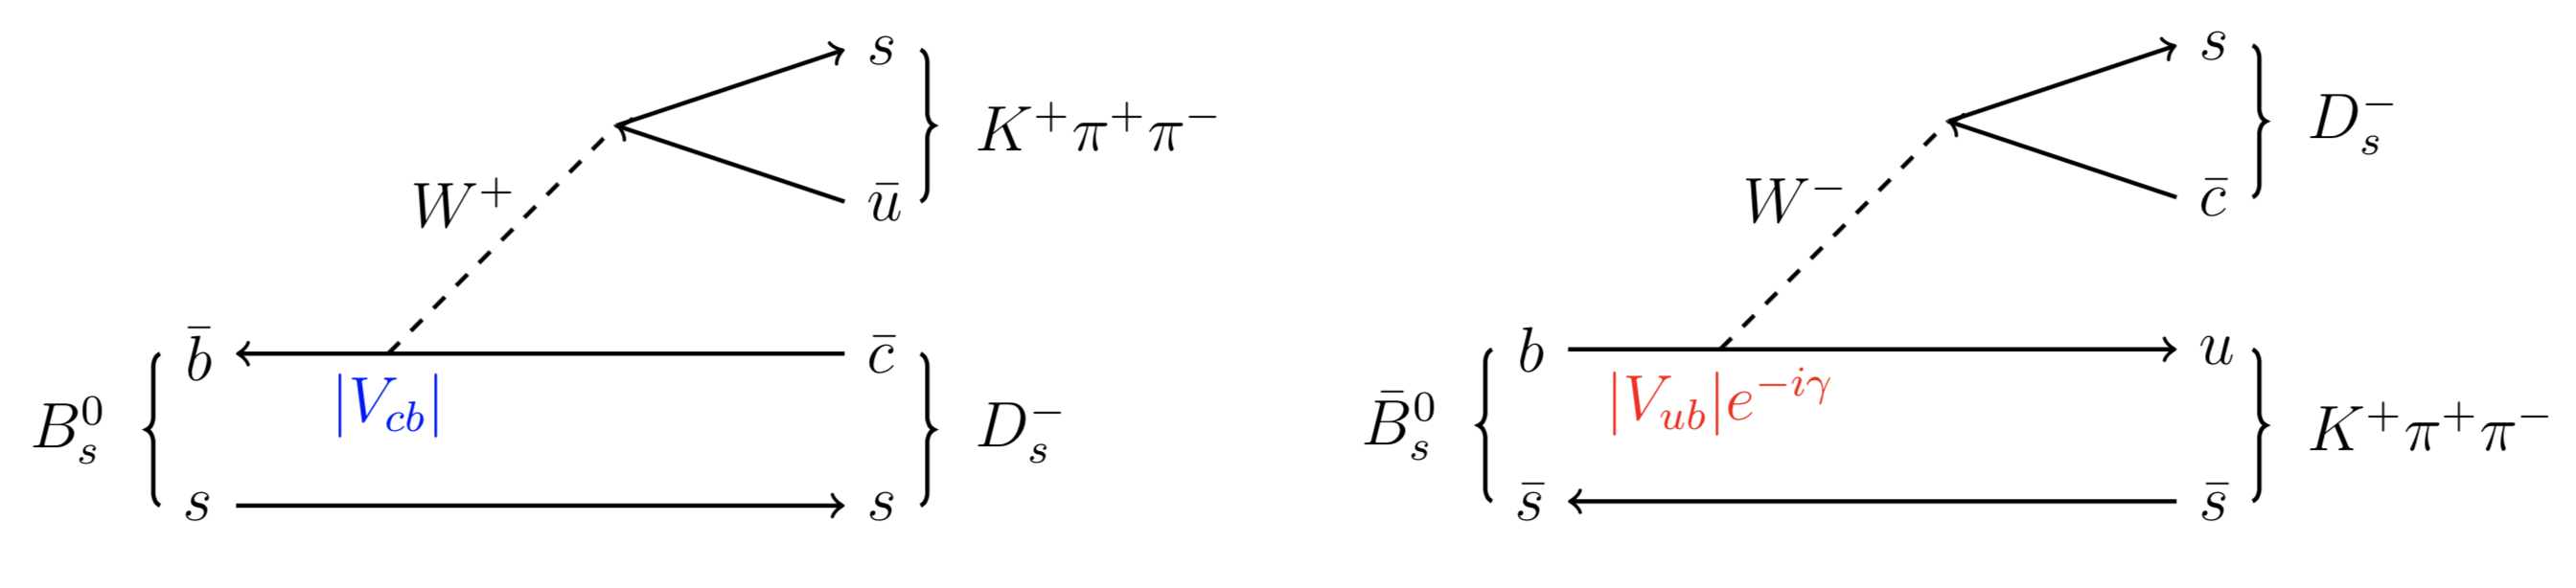
\includegraphics[height=!,width=\textwidth]{figs/feynman.png}
\caption{Feynman diagram for $B_s^0/\bar B_s^0 \to D_s^- K^+ \pip \pim$ decays.}
\label{fig:decay_feynman}
\end{figure}


%\begin{figure}[h]
%\centering
%%\tikzsetnextfilename{feynman_mixing.pdf}
%\begin{tikzpicture}[scale=1.]
%%Strange to beauty quark
%\draw [->,thick] (0,0) node[left]{$s$} -- (4,0) node[right]{$b$};
%%Beauty to strange Anti Quark
%\draw [<-,thick] (0,1) node[left]{$\bar{b}$} -- (4,1) node[right]{$\bar{s}$};
%%W boson
%\draw [dashed,thick] (2.5,0) -- (2.5,1);
%\draw [dashed,thick] (1.5,0) -- (1.5,1);
%
%%Labels
%\draw[decoration={brace},decorate,thick] (-0.5,0) -- node[left=0.2] {$B_s^0$} (-0.5,1);
%\draw[decoration={brace},decorate,thick] (4.5,1) -- node[right=6pt] {$\bar{B}_s^0$} (4.5,0);
%\node at (1.2,0.5) {$W$};
%\node at (2.8,0.5) {$W$};
%\node at (2,-0.3) {$u,c,t$};
%\node at (2,1.3) {$u,c,t$};
%\end{tikzpicture}
%\caption{Feynman diagram of $B_s$ mixing process.}
%\label{fig:mixing_feynman}
%\end{figure}
%
%
%\begin{figure}[h]
%\centering
%   
%\begin{subfigure}[b]{0.45\textwidth}
%
%\begin{tikzpicture}[scale=1]
%%Strange quark
%\draw [->,thick] (0,0) node[left]{$s$} -- (4,0) node[right]{$s$};
%%Beauty to Charm Quark
%\draw [<-,thick] (0,1) node[left]{$\bar{b}$} -- (4,1) node[right]{$\bar{c}$};
%\node at (1.,0.66) {$\textcolor{blue}{\vert V_{cb} \vert}$};
%
%%W+ boson
%\draw [dashed,thick] (1,1) -- (2.5,2.5);
%\node at (1.5,2) {$W^+$};
%%u Quark
%\draw [->,thick] (2.5,2.5) -- (4,3) node[right]{$s$};
%%d Quark
%\draw [<-,thick](2.5,2.5) -- (4,2) node[right]{$\bar{u}$};
%
%%pipipi brace and node
%\draw[decoration={brace},decorate,thick](4.5,3) -- node[right=6pt] {$K^+\pi^+\pi^-$} (4.5,2);
%%Ds brace and node
%\draw[decoration={brace},decorate,thick] (4.5,1) -- node[right=6pt] {$D_s^-$} (4.5,0);
%%Bs brace and node
%\draw[decoration={brace},decorate,thick] (-0.5,0) -- node[left=0.2] {$B_s^0$} (-0.5,1);
%\end{tikzpicture}
%
%\end{subfigure} \hfill
%%
%%
%%
%%
%%
%\begin{subfigure}[b]{0.45\textwidth}
%
%\begin{tikzpicture}[scale=1]
%%Strange quark
%\draw [<-,thick] (0,0) node[left]{$\bar s$} -- (4,0) node[right]{$\bar s$};
%%Beauty to Charm Quark
%\draw [->,thick] (0,1) node[left]{$b$} -- (4,1) node[right]{$u$};
%\node at (1.,0.66) {$\textcolor{red}{\vert V_{ub} \vert e^{-i\gamma}}$};
%%W+ boson
%\draw [dashed,thick] (1,1) -- (2.5,2.5);
%\node at (1.5,2) {$W^-$};
%%u Quark
%\draw [->,thick] (2.5,2.5) -- (4,3) node[right]{$s$};
%%d Quark
%\draw [<-,thick](2.5,2.5) -- (4,2) node[right]{$\bar{c}$};
%
%%pipipi brace and node
%\draw[decoration={brace},decorate,thick](4.5,3) -- node[right=6pt] {$D_s^-$} (4.5,2);
%%Ds brace and node
%\draw[decoration={brace},decorate,thick] (4.5,1) -- node[right=6pt] {$K^+\pi^+\pi^-$} (4.5,0);
%%Bs brace and node
%\draw[decoration={brace},decorate,thick] (-0.5,0) -- node[left=0.2] {$\bar B_s^0$} (-0.5,1);
%\end{tikzpicture}
%
%\end{subfigure}
%\caption{Feynman diagram for $B_s^0/\bar B_s^0 \to D_s^- K^+ \pip \pim$ decays.}
%\label{fig:decay_feynman}
%
%\end{figure}

\section{Data samples}

We use the full Run 1 sample from Stripping 21, consisting of 3 $\invfb$ of data, collected in the years 2011 and 2012 at a center of mass energies of 7 $\tev$ and 8 $\tev$, respectively. 
The selected $\Bs$-candidates are required to pass the L0 XXX trigger. Events that pass the L0 stage are further required to pass the HLT1 XXX trigger. 
All remaining candidates have to pass either the 2, 3 or 4-body topological trigger (TOS). \newline
For the presented analysis the B02DKPiPiD2HHHPIDBeauty2CharmLine is used to preselect signal $\Bs\to\Ds\kaon\pion\pion$ candidates. 
A summary of the cuts employed by this stripping line can be found in Table \ref{table:StrippingCuts}.      


\begin{table}[h]
\centering
 \begin{tabular}{l l}
Variable & Stripping Cut\\
  \hline
Track $\chi^{2}$/nDoF & $<$ 3\\
Track $\ptot$ & $>$ 1000 $\mevc$\\
Track $\pt$ & $>$ 100 $\mevc$\\
Track IP $\chi^{2}$ & $>$ 4\\
$\Ds$ Daughter $\pt$ & $\Sigma_{i=1}^{3} p_{i} > 1800 \mevc$\\
$\Ds$ Daughter DOCA & 0.5 $\mm$\\
$\Ds$ mass $m_{\Ds}$  & within $\pm$ 50 $\mevcc$ of PDG value\\
$\Ds$ Vertex $chi^{2}$/nDoF & $<$ 10\\
$\Ds$ min FD $chi^{2}$ & $>$ 36\\
$X_{s}$ Daughter DOCA & 0.4 $\mm$\\
$X_{s}$ Daughter $\pt$ & $\Sigma_{i=1}^{3} p_{t,i} > 1250 \mevc$\\
$X_{s}$ Vertex $chi^{2}$/nDoF & $<$ 8\\
$X_{s}$ min FD $chi^{2}$/nDoF & $>$ 16\\
$X_{s}$ DIRA & $>$ 0.98\\
$X_{s}$ $\Delta\rho$ & $>$ 0.1 $\mm$\\
$X_{s}$ $\Delta Z$ & $>$ 2.0 $\mm$\\
$\Bs$ DIRA & $>$ 0.98\\
$\Bs$ min IP $\chi^{2}$ & $>$ 25\\
$\Bs$ Vertex $chi^{2}$/nDoF & $<$ 10\\
$\Bs$ $\tauBs$ & $>$ 0.2 $\ps$\\
$\kaon$ \dllkpi & $>$ -5\\
$\pion$ \dllkpi & $<$ 10\\
\end{tabular}
\caption{Summary of the stripping selections for $\Bs\to\Ds\kaon\pion\pion$ decays.}
\label{table:StrippingCuts}
\end{table}


\section{Simulated samples}

\begin{table}[h]
\centering
 \begin{tabular}{l l l}
Quantity & $\Bs\to\Ds\kaon\pion\pion$ & $\Bs\to\Ds\pion\pion\pion$\\
\hline
event type     & 1326607   & 1326606\\
events generated & 1,131,662 & 1,188,549\\
events selected  & 14480     & 15793\\
\end{tabular}
\caption{Generated and selected MC events for signal and normalization channel at $\sqs = 7\mbox{ }TeV$.}
\label{table:MC11}
\end{table}

\begin{table}[h]
\centering
 \begin{tabular}{l l l}
Quantity & $\Bs\to\Ds\kaon\pion\pion$ & $\Bs\to\Ds\pion\pion\pion$\\
  \hline
event type       & 1326607   & 1326606\\
events generated & 1,257,244 & 1,167,428\\
events selected  & 14422     & 13423\\ 
\end{tabular}
\caption{Generated and selected MC events for signal and normalization channel at $\sqs = 8\mbox{ }TeV$.}
\label{table:MC12}
\end{table}

The simulated (MC) samples are generated using Pythia 8 with Sim08 and Gauss v45r11. Samples are reconstructed with Brunel v43r2p11 and the DSTs were processed using DaVinci v36r1p1. 
The event numbers for the simulated $\Bs\to\Ds\kaon\pion\pion$ and $\Bs\to\Ds\pion\pion\pion$ samples, as well as the amount of generated and selected events, 
is shown in Tab. \ref{table:MC11} and \ref{table:MC12} for the different center of mass energies. \newline
In order to use our MC samples during the BDT training, described in Chapter \ref{sec:Selection}, and the calculation of efficiencies (Chapter \ref{sec: efficiency}), 
we have to ensure that the $\Bs\to\Ds\kaon\pion\pion$ decay is modelled correctly by the simulation. 
To check this, we compare distributions of observables which we use during the multivariate selection stage, as well as some key event observables. 
The compared distributions need to be generated by signal decays only, therefore we truth-match all particles in the MC samples. 
Signal distributions of observables in data are obtained using the sWeight technique \cite{Pivk:2004ty}. 
Due to the lack of a clear signal peak in the $\Bs\to\Ds\kaon\pion\pion$ data after the stripping, trigger and cut-based preselection, we use preselected $\Bs\to\Ds\pion\pion\pion$ candidates to obtain signal sWeights:  
We perform a fit of a Gaussian signal model and an exponential background to the invariant mass distribution of $\Bs\to\Ds\pion\pion\pion$ candidates. 
Using the weights generated from this fit, we weight the distributions of data observables in $\Bs\to\Ds\kaon\pion\pion$ and obtain the corresponding signal distributions. \newline
Figure \ref{fig: MCbeforeWeighting} shows the distribution of the number of tracks per event and the distribution of the maximum ghost probability over all tracks in MC and data.

\begin{figure}[h]
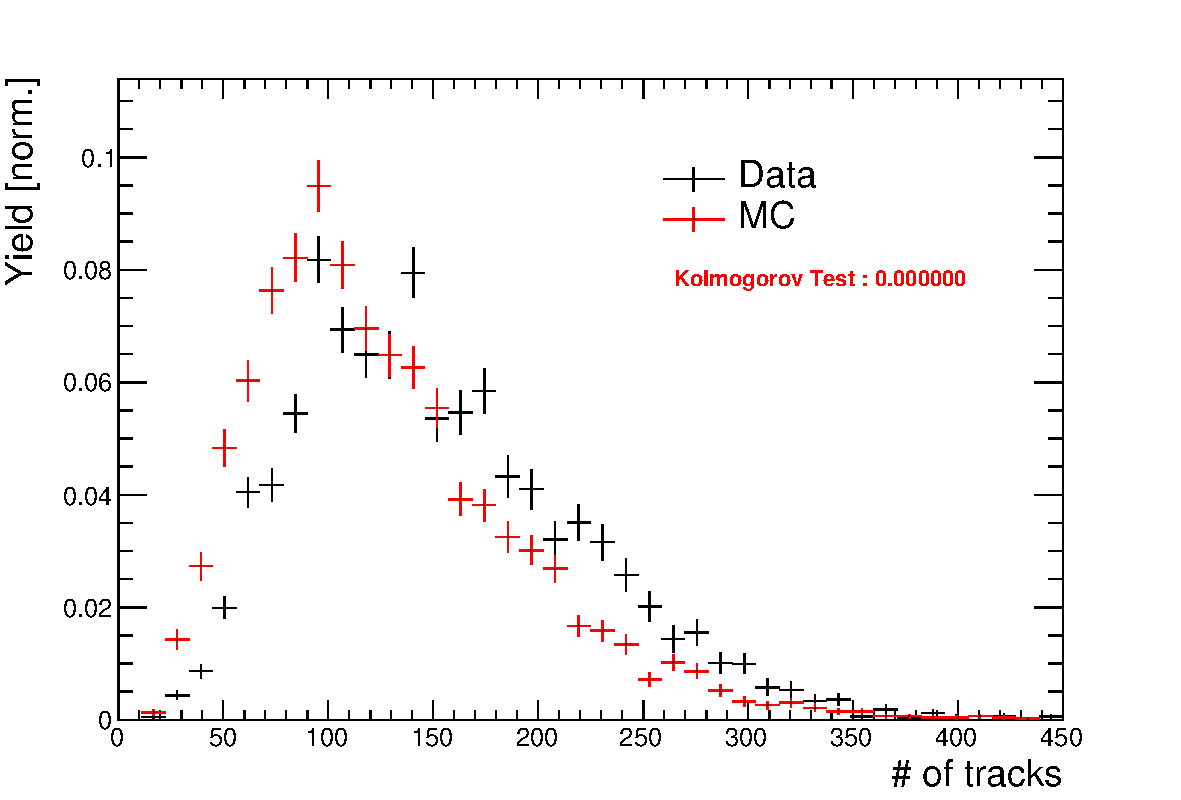
\includegraphics[height=6.cm,width=0.45\textwidth]{figs/nTracks.pdf}
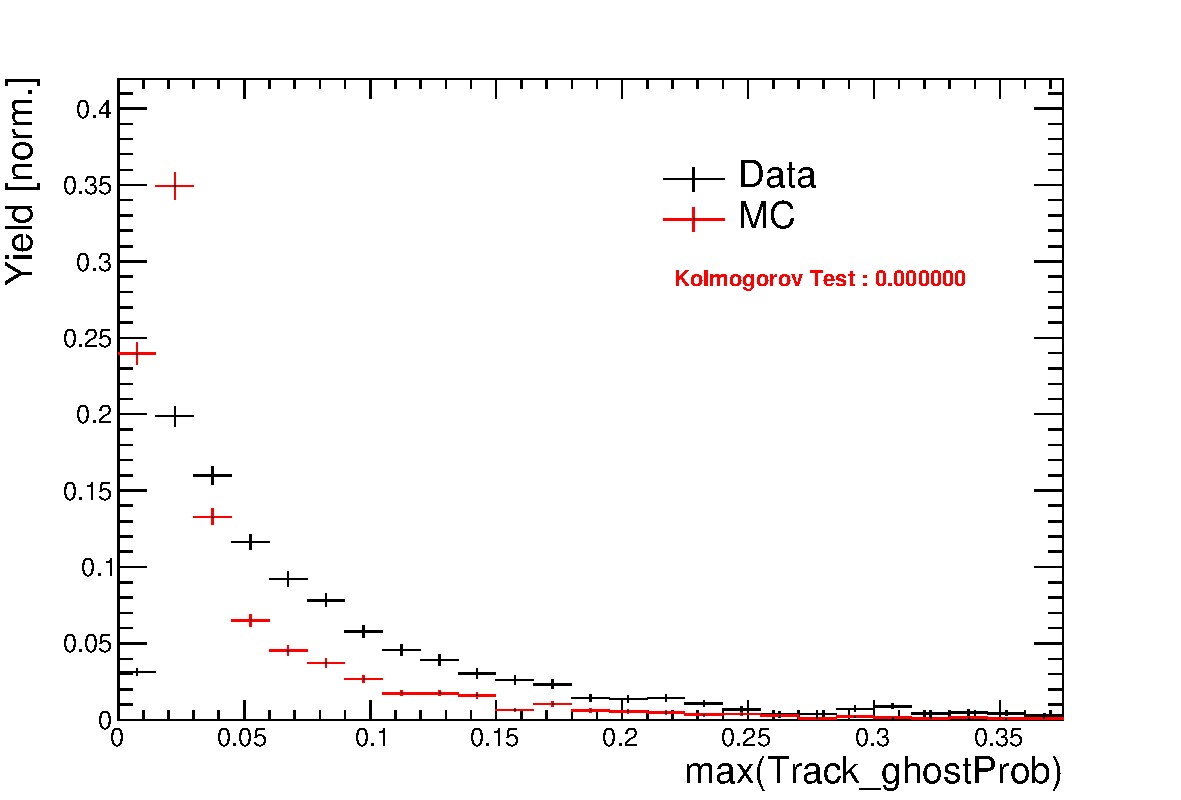
\includegraphics[height=6.cm,width=0.45\textwidth]{figs/max_ghostProb.pdf}
\caption{Comparison between the distribution of (left) the number of tracks and (right) the maximum ghost probability over all tracks in (black) data and (red) simulation.}
\label{fig: MCbeforeWeighting}
\end{figure}


In both cases, the distributions differ significantly. Therefore, we reweight the MC samples using those two variables. 
The reweighting is done successively, e.g. we perform two 1D weighting processes, where we equalize the respective MC distribution to the observed distribution in data.  
All distributions of observables used in the BDT training, before and after the reweighting procedure, are shown in the Appendix \ref{sec: mcvdata}.                 


\section{Selection}
\label{sec:Selection}

For the presented analysis, we reconstruct the $\Bs\to\Ds\kaon\pion\pion$ decay through three different final states of the $\Ds$ meson, $\Ds\to\kaon\kaon\pion$, $\Ds\to\kaon\pion\pion$ and $\Ds\to\pion\pion\pion$.
Of those three final states $\Ds\to\kaon\kaon\pion$ is the most prominent one,
 while $\mathcal{BR}(\Ds\to\pion\pion\pion) \approx 0.2\cdot\mathcal{BR}(\Ds\to\kaon\kaon\pion)$ and $\mathcal{BR}(\Ds\to\kaon\pion\pion) \approx 0.1\cdot\mathcal{BR}(\Ds\to\kaon\kaon\pion)$ holds for the other two. \newline
A two-fold approach is used to isolate the $\Bs\to\Ds\kaon\pion\pion$ candidates from data passing the stripping line. 
First, further one-dimensional cuts are applied to reduce the level of combinatorial background and to veto some specific physical background. 
This stage is specific to the respective final state in which the $\Ds$ meson is reconstructed, since different physical backgrounds, depending on the respective final state, have to be taken into account.   
After that, a multivariate classifier is trained which combines the information of several input variables, including their correlation, into one powerful discriminator
between signal and combinatorial background. For this stage, all possible $\Ds$ final states are treated equally. 

\subsection{Cut-based selection}

In order to minimize the contribution of combinatorial background to our samples, we apply the following cuts to the b hadron:

\begin{itemize}

\item DIRA $>$ 0.99994

\item min IP $\chi^{2}$ $<$ 20 to any PV,

\item FD $\chi^{2}$ $>$ 100 to any PV,

\item Vertex $\chi^{2}$/nDoF $<$ 8,

\item ($Z_{\Ds}-Z_{\Bs}$) $>$ 0 , where $Z_{M}$ is the z-component of the position $\vec{x}$ of the decay vertex for the $\Bs$/$\Ds$ meson.

\end{itemize}    


Additionally, we veto various physical backgrounds, which have either the same final state as our signal decay, or can contribute via a single misidentification of $\kaon\to\pion$ or $\kaon\to\proton$. 
In the following, the vetoes are ordered by the reconstructed $\Ds$ final state they apply to: 


\begin{enumerate}

\item All:

\begin{enumerate}

\item $\Bs\to\Dsp\Dsm$ : $|M(\kaon\pion\pion) - m_{\Ds}| >$ 20 $\mevcc$.

\item $\Bs\to\Ds^{-}\Kp\Km\pip$ : possible with single missID of $\Km\rightarrow\pim$, rejected by requiring $\pim$ to fulfill $\dllkpi$ $<$ 5. 

\end{enumerate}

\item $\Ds\to\kaon\kaon\pion$

\begin{enumerate}

\item $\Bz\to\Dp(\to\Kp\pim\pip)\kaon\pion\pion$ : possible with single missID of $\pip\rightarrow\Kp$, vetoed by changing particle hypothesis and recompute $|M(\Kp\pim\pip) - m_{Dp}|$ $>$ 30 $\mevcc$, 
or the $\Kp$ has to fulfill $\dllkpi$ $>$ 10.

\item $\Lb\to\Lc(\to\proton\Km\pip)\kaon\pion\pion$ : possible with single missID of $\proton\rightarrow\Kp$, vetoed by changing particle hypothesis and recompute $M(\proton\Km\pip) - m_{\Lc}$ $>$ 30 $\mevcc$, 
or the $\Kp$ has to fulfill ($\dllkpi$ - $\dllppi$) $>$ 5.

\item $\Dz\to\kaon\kaon$ : $\Dz$ combined with a random $\pion$ can fake a $\Ds\to\kaon\kaon\pion$ decay and be a background to our signal, vetoed by requiring $M(\kaon\kaon) < 1840 \mevcc$. 

\end{enumerate}

\item $\Ds\to\kaon\pion\pion$

\begin{enumerate}

\item $\Dz\to\pip\Km$ : $\Dz$ combined with a random $\pim$ can fake a $\Ds^{-}\to\Km\pip\pim$ decay and be a background to our signal, vetoed by requiring $M(\pip\Km) < 1750 \mevcc$.

\item $\Lb\to\Lc(\to\proton\pim\pip)\kaon\pion\pion$ : possible with single missID of $\proton\rightarrow\Kp$, vetoed by changing particle hypothesis and recompute $M(\proton\pim\pip) - m_{\Lc}$ $>$ 30 $\mevcc$, 
or the $\Kp$ has to fulfill ($\dllkpi$ - $\dllppi$) $>$ 5.

\end{enumerate}

\item $\Ds\to\pion\pion\pion$

\begin{enumerate}

\item $\Dz\to\pion\pion$ : combined with a random $\pion$ can fake a $\Ds\to\pion\pion\pion$ decay and be a background to our signal, vetoed by requiring both possible combinations to have $M(\pion\pion) < 1700 \mevcc$.

\end{enumerate}

\end{enumerate}


The most prominent final state used in this analysis is $\Bs\to\Ds(\to\kaon\kaon\pion)\kaon\pion\pion$, 
where the $\Ds$ decay can either proceed via the narrow $\phiz$ resonance, the broader $\Kstarz$ resonance, or non resonant.
Depending on the decay process being resonant or not, we apply additional PID requirements on this final state:

\begin{itemize}

\item resonant case: 
\begin{itemize}
\item $\Dsp\to\phiz\pip$, with $|M(\Kp\Km) - m_{\phiz}|$ $<$ 20 $\mevcc$ : no additional requirements, since $\phiz$ is narrow and almost pure $\Kp\Km$. 
\item $\Dsp\to\Kstarzb\Kp$, with  $|M(\Km\pip) -m_{\Kstarz}|$ $<$ 75 $\mevcc$ :  $\dllkpi$ $>$ 0 for kaons, since this resonance is more than ten times broader than $\phiz$. 
\end{itemize}

\item non resonant case: $\dllkpi$ $>$ 5 for kaons, since the non resonant category has significant charmless contributions.

\end{itemize}



For the other two final states, we apply global PID requirements:



\begin{itemize}

\item  $\Ds\to\kaon\pion\pion$

\begin{itemize}

\item  $\dllkpi$ $>$ 10 for kaons, since we expect significantly higher charmless background contribution in this channel. 

\item  $\dllkpi$ $<$ 5 for pions.

\end{itemize}

\item $\Ds\to\pion\pion\pion$

\begin{itemize}

\item $\dllkpi$ $<$ 10 for all pions.

\item $\dllppi$ $<$ 10 for all pions.

\end{itemize}

\end{itemize}


%Since a measurement of the weak CKM phase $\gamma$ in the $\Bs\to\Ds\kaon\pion\pion$ channel will almost certainly be statistically limited, 
%we plan to add also the $\Ds\to\pion\pion\pion$ final state with $\mathcal{BR}(\Ds\to\pion\pion\pion) \approx 0.2\cdot\mathcal{BR}(\Ds\to\kaon\kaon\pion)$ to the $\gamma$ analysis. 
%Since the determination of the branching ratio is expected to have the same level of statistical and systematical uncertainties and due to the additional complexity (different selection, efficiencies, simulated samples), 
%we choose to only use the most prominent $\Ds\to\kaon\kaon\pion$ final state for the BR determination. 


\subsection{Multivariate stage}

We use TMVA \cite{Hocker:2007ht} to train a multivariate discriminator, which is used to further improve the signal to background ratio. 
The 17 variables used for the training are:

\begin{itemize} 

\item max(ghostProb) over all tracks

\item cone($\pt$) asymmetry of every track, 
which is defined to be the difference between the $\pt$ of the $\pi$/$\kaon$ and the sum of all other $\pt$ in a cone of radius $r = \sqrt{(\Delta\Phi)^{2} + (\Delta\eta)^{2}}$ $<$ 1 rad around the signal $\pi$/$\kaon$ track.

\item min(IP$\chi^{2}$) over the $X_{s}$ daughters

\item max(DOCA) over all pairs of $X_{s}$ daughters

\item min(IP$\chi^{2}$) over the $\Ds$ daughters

\item $\Ds$ and $\Bs$ DIRA

\item $\Ds$ FD significance

\item max($\cos(\Ds h_{i})$), where $\cos(\Ds h_{i})$ is the cosine of the angle between the $\Ds$ and another track i in the plane transverse to the beam

\item $\Bs$ IP$\chi^{2}$, FD$\chi^{2}$ and Vertex $\chi^{2}$

\end{itemize}

Various classifiers were investigated in order to select the best performing discriminator. Consequently, a boosted decision tree with gradient boost (BDTG) is chosen as nominal classifier. 
We use truth-matched MC as signal input. 
Simulated signal candidates are required to pass the same trigger, stripping and preselection requirements, that were used to select the data samples.  
For the background we use events from the high mass sideband ($m_{\Bs candidate}$ $>$ 5600 $\mevcc$) of our data samples. 
As shown in Fig. \ref{fig:massforBDT}, this mass region is sufficiently far away from signal structures and is expected to be dominantly composed of combinatorial background. \newline

\begin{figure}[h]
%\vspace*{-0.4cm}
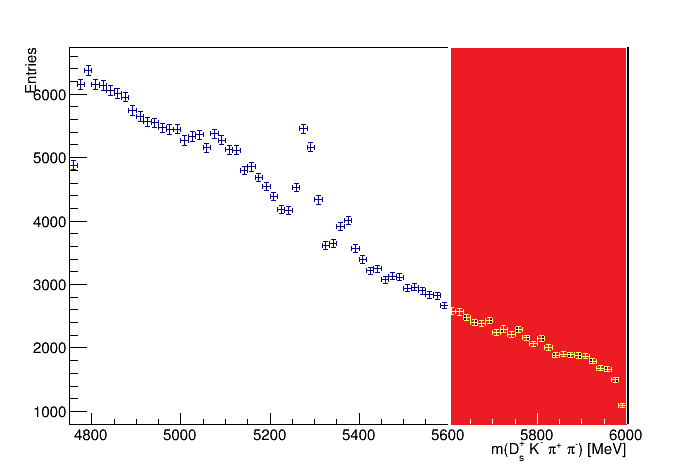
\includegraphics[height=7.4cm,width=0.7\textwidth]{figs/mass_Bs_forBDT_12_AnA.png}
%\vspace*{-0.2cm}
\caption{Invariant mass distribution of preselected $\Bs\to\Ds\kaon\pion\pion$ candidates. The red coloured region with $m_{\Bs candidate}$ $>$ 5600 $\mevcc$ is used as background input for the boosted decision tree.}
\label{fig:massforBDT}
\end{figure}

The distributions of the input variables for signal and background are shown in Fig. \ref{fig:BDT_Input_1}. 

\begin{figure}[h]
%\vspace*{-0.4cm}
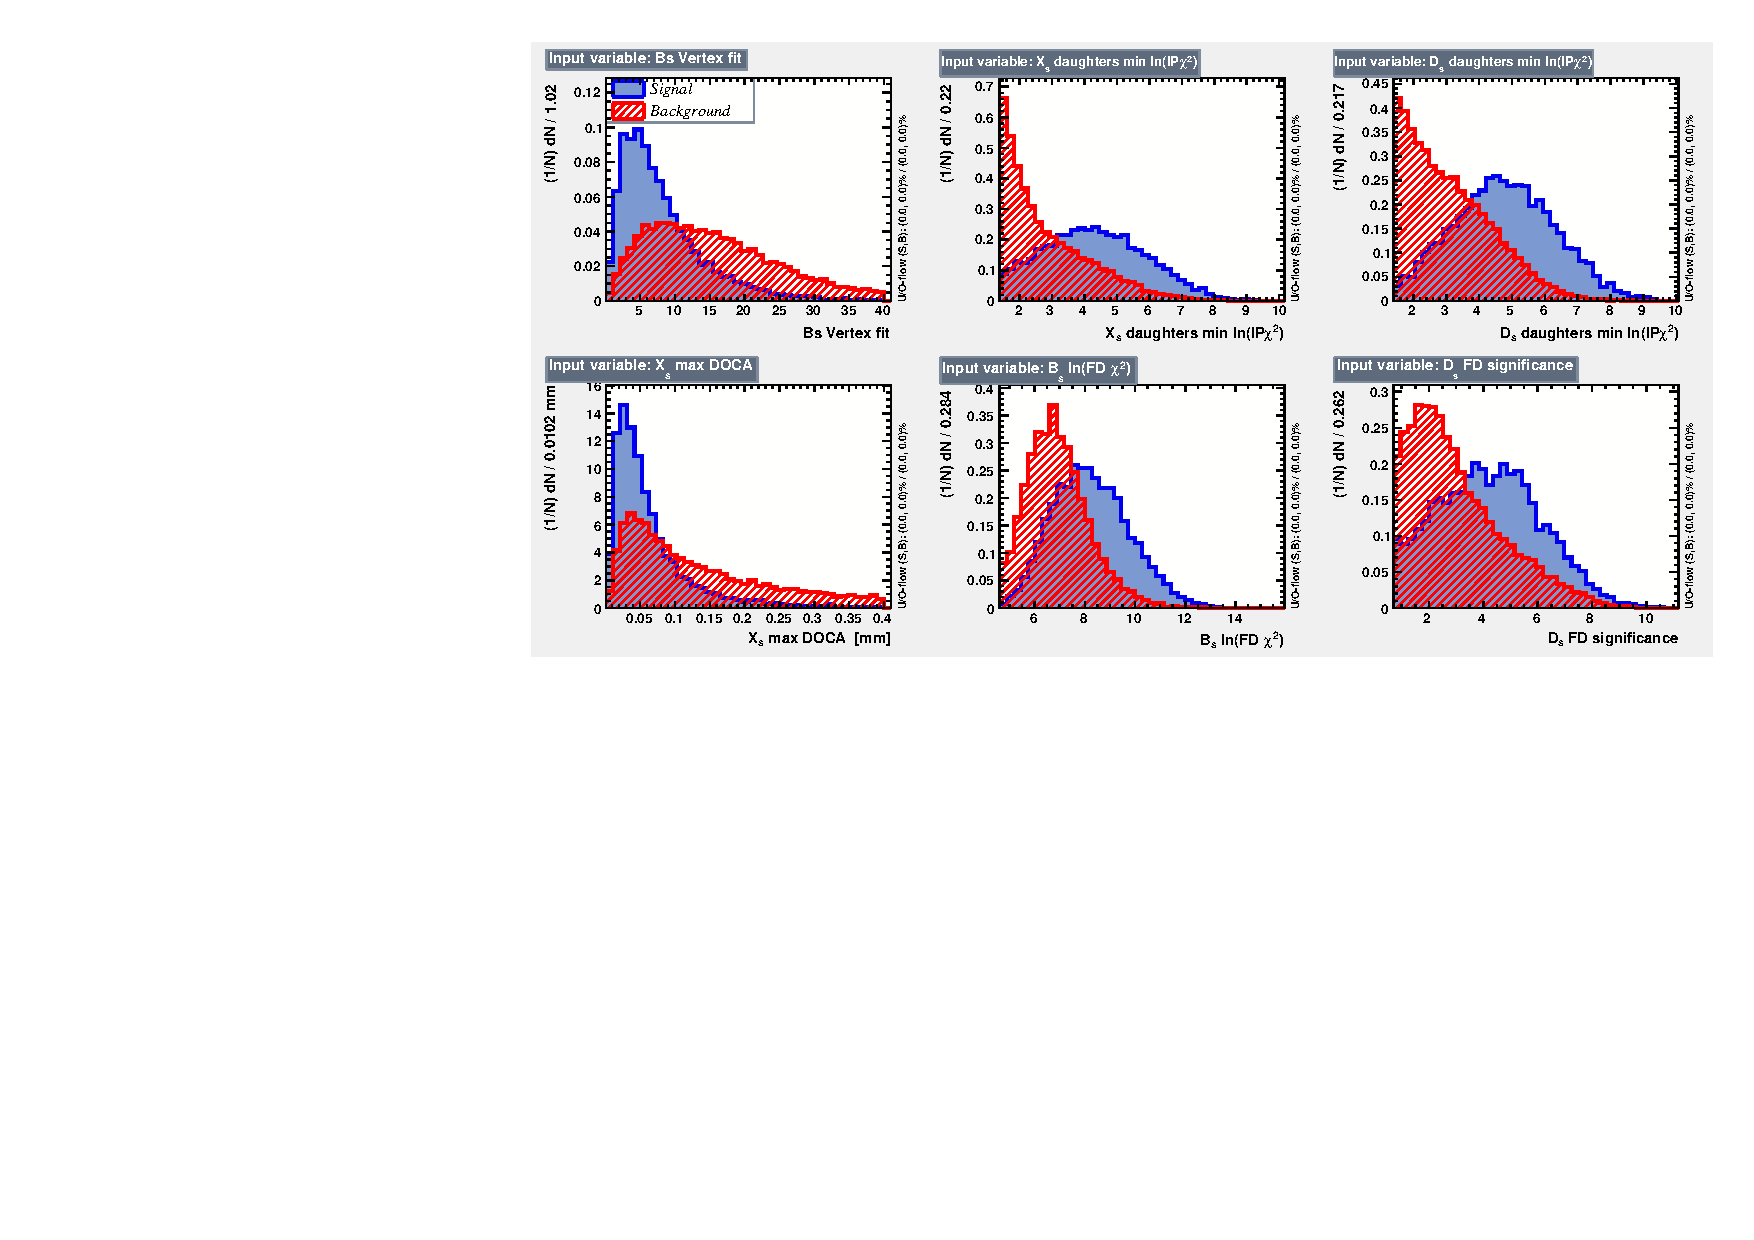
\includegraphics[height=6.cm,width=0.95\textwidth]{figs/BDT_Input_1.pdf}
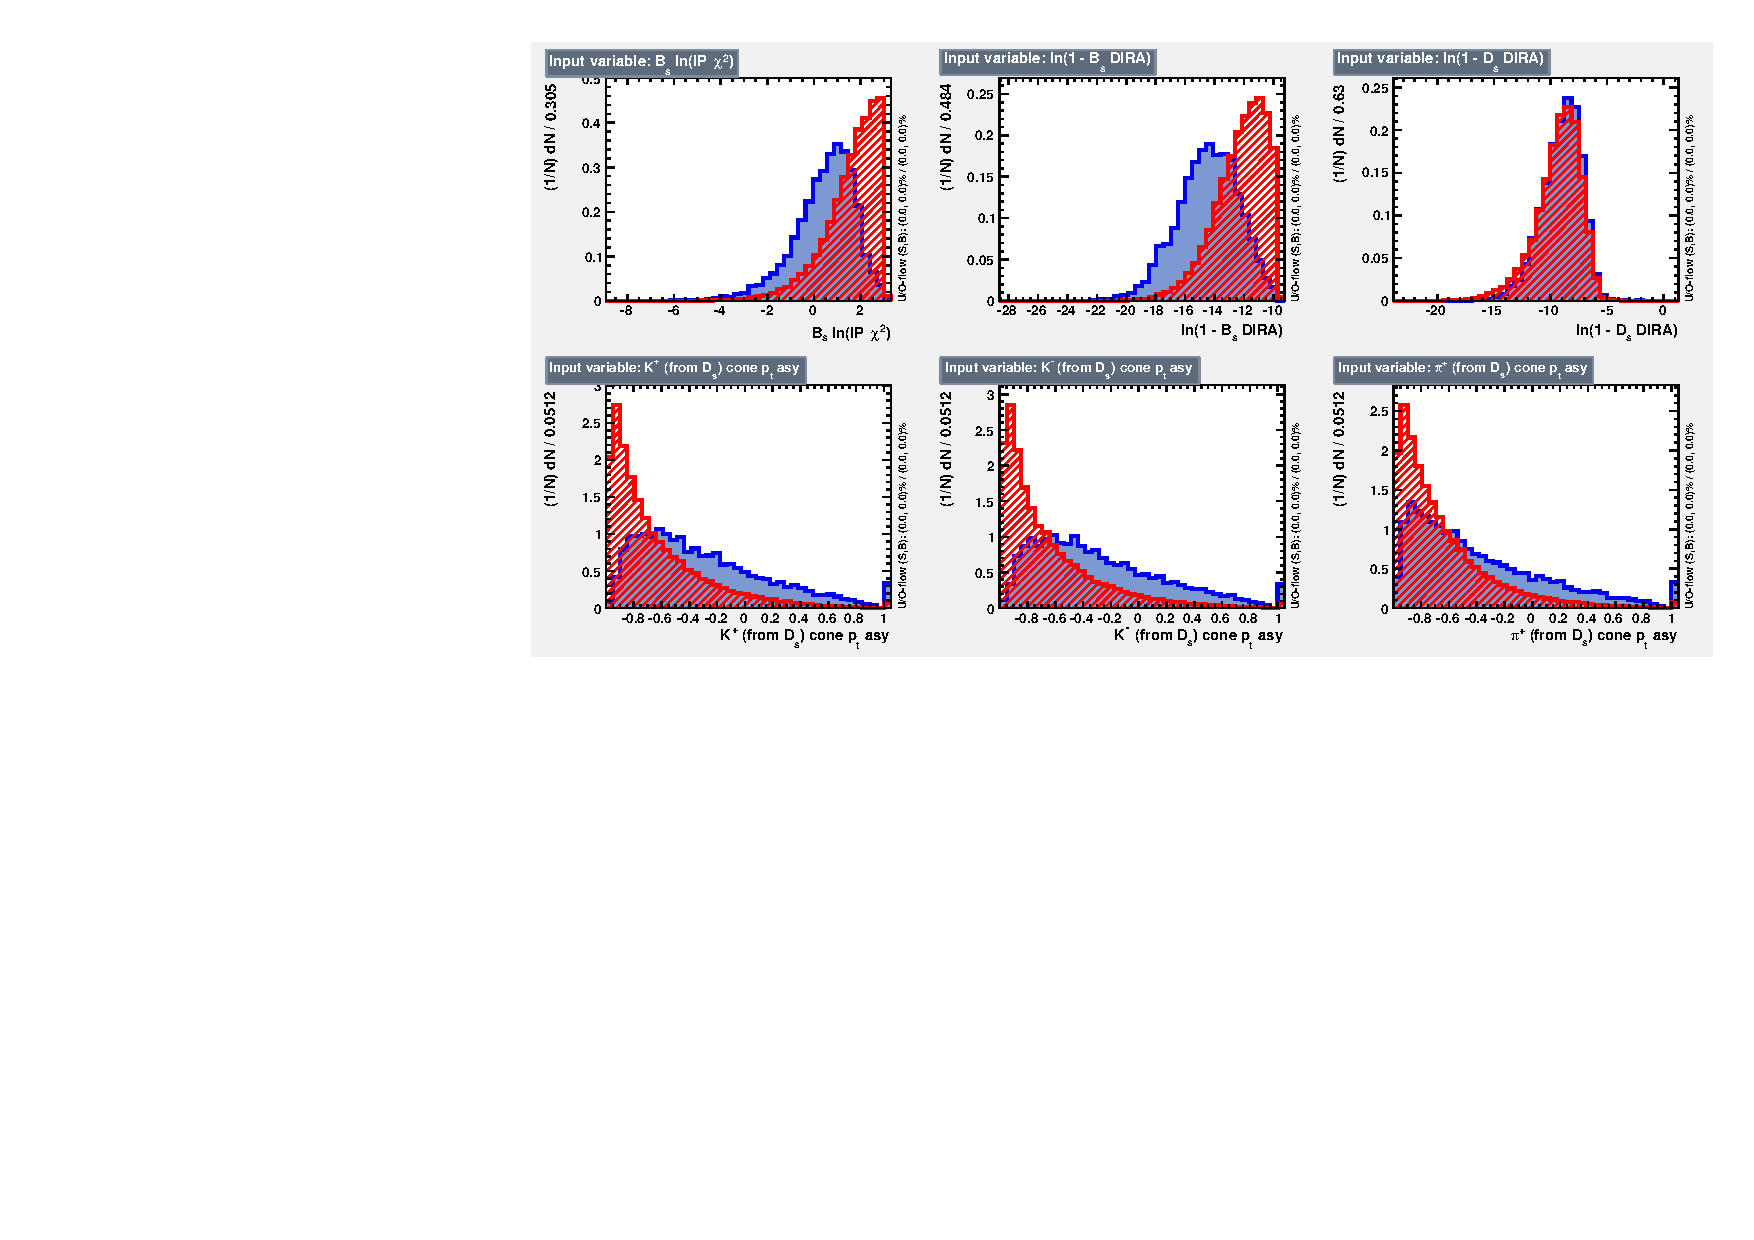
\includegraphics[height=6.cm,width=0.95\textwidth]{figs/BDT_Input_2.pdf}
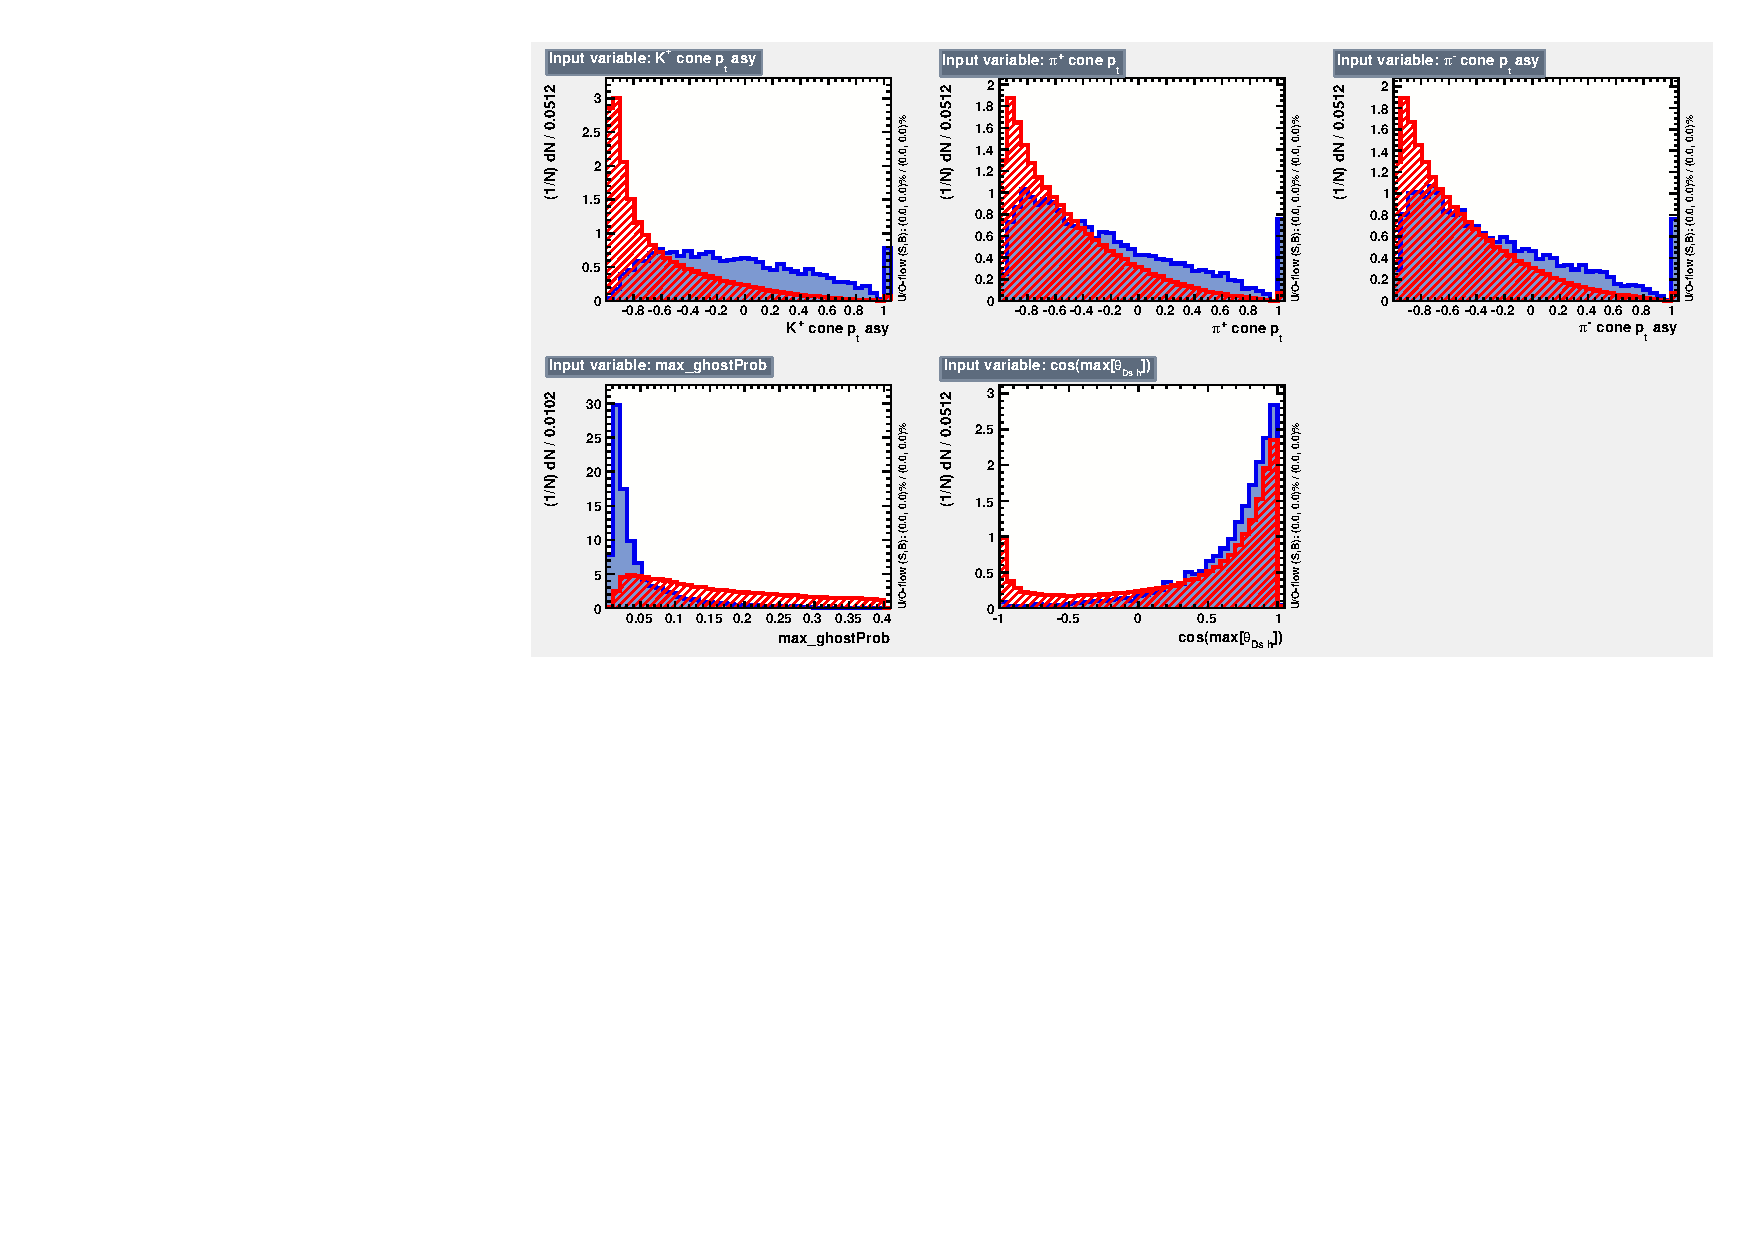
\includegraphics[height=6.cm,width=0.95\textwidth]{figs/BDT_Input_3.pdf}
%\vspace*{-0.2cm}
\caption{Distributions of the input variables used in the BDTG training. The background is shown as red hatched, while the signal is depicted solid blue.}
\label{fig:BDT_Input_1}
\end{figure}


The relative importance of the input variables for the BDTG training is summarized in Table \ref{table:InputVars}.

\begin{table}[h]
\centering
 \begin{tabular}{l c}
Variable & relative importance [$\%$]\\
  \hline
pi\_minus\_ptasy\_1.00 & 7.32\\
log\_Ds\_FDCHI2\_ORIVX & 7.23\\
K\_plus\_ptasy\_1.00 & 7.17\\
log\_Ds\_DIRA & 6.96\\
Bs\_ENDVERTEX\_CHI2 & 6.82\\
max\_ghostProb & 6.76\\
pi\_plus\_ptasy\_1.00 & 6.57\\
log\_DsDaughters\_min\_IPCHI2 & 6.21\\
log\_Bs\_DIRA & 6.15\\
K\_plus\_fromDs\_ptasy\_1.00 & 6.10\\
log\_XsDaughters\_min\_IPCHI2 & 5.87\\
K\_minus\_fromDs\_ptasy\_1.00 & 5.62\\
cos(Ds h) & 5.58\\
log\_Bs\_IPCHI2\_OWNPV & 5.08\\
log\_Bs\_FDCHI2\_OWNPV & 4.04\\
Xs\_max\_DOCA & 3.98\\
pi\_minus\_fromDs\_ptasy\_1.00 & 2.59\\
\end{tabular}
\caption{Summary of the relative importance of each variable in the training of the BDTG.}
\label{table:InputVars}
\end{table}

 
The BDTG output distribution for test and training samples is shown in Fig \ref{fig:BDT_Response}. No sign of overtraining is observed. 

\begin{figure}[h]
%\vspace*{-0.4cm}
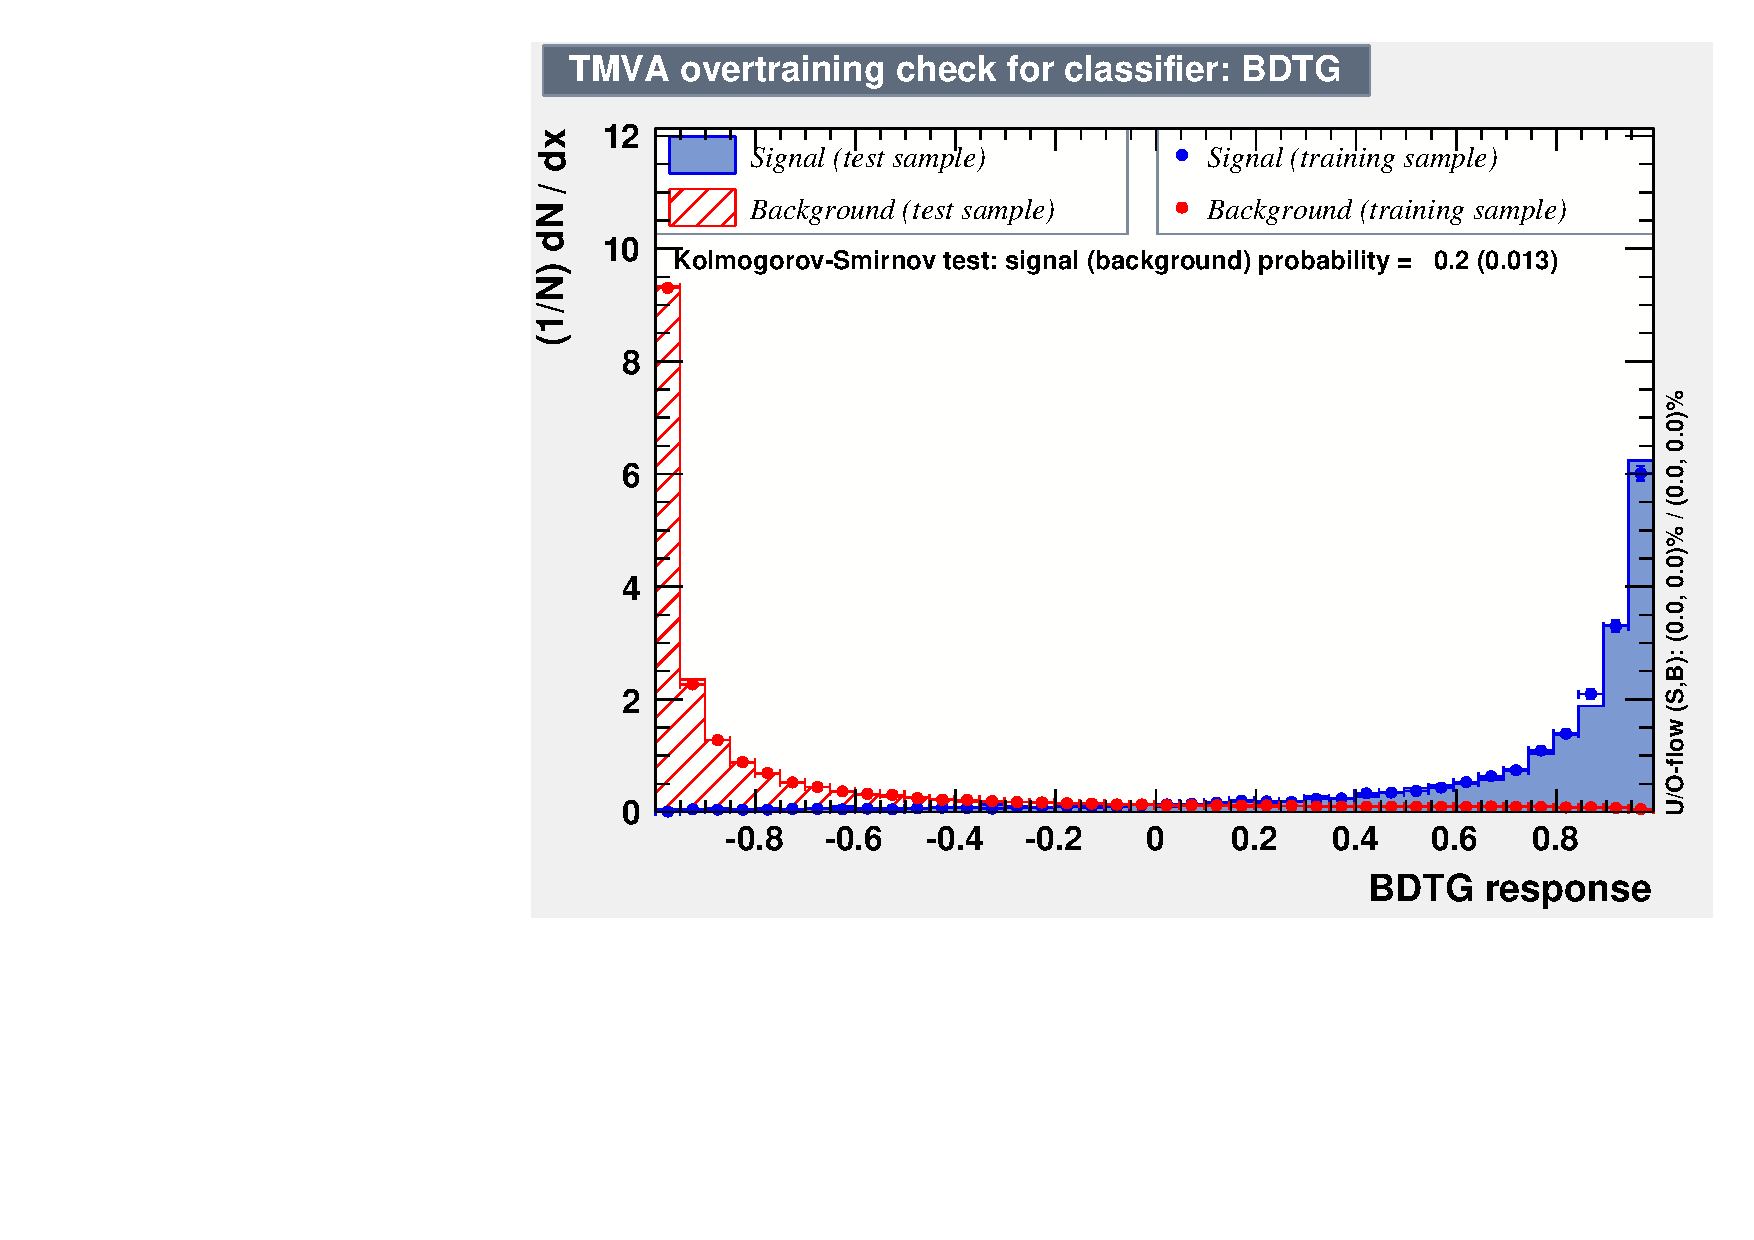
\includegraphics[height=7.4cm,width=0.7\textwidth]{figs/BDT_Response_new.pdf}
%\vspace*{-0.2cm}
\caption{BDTG output classifier distribution for (blue) signal and (red) background. The response of an independent test sample (dots) is overlaid.}
\label{fig:BDT_Response}
\end{figure}


       
We determine the optimal cut value by maximizing the figure of merit $S/\sqrt{S+B}$ where S is the signal yield and B the background yield in the signal region, defined to be within $\pm$50 $\mevcc$ of the nominal $\Bs$ mass. 
To avoid a bias in the determination of the branching fraction, we determine S and B using our normalization channel. 
All trigger, stripping and additional selection criteria described in this and the previous chapter are applied to the $\Bs\to\Ds\pion\pion\pion$ data samples. 
After that, we perform a simplified version of the fit to the invariant mass distribution of $\Bs\to\Ds\pion\pion\pion$ candidates described in Sec.~\ref{sec: fitting}.
Here, a Gaussian function to model the signal and an exponential function to model combinatorial background is used.
From this fit we estimate the number of signal events in our normalization channel. 
Multiplying that number with the PDG branching fraction of $\frac{\mathcal{B}(\Bs\to\Ds\kaon\pion\pion)}{\mathcal{B}(\Bs\to\Ds\pion\pion\pion)}$ and the ratio of efficiencies discussed in Sec. \ref{sec: efficiency} allows us to estimate the expected number of $\Bs\to\Ds\kaon\pion\pion$ signal decays. The number of background events can then be computed as

\begin{equation}
 N_{bkg}=N_{all}-N_{sig}|_{m_{\Bs\pm50\mevcc}}.   
\end{equation}

The efficiency curves as a function of the cut value are shown in Fig. \ref{fig:BDT_Efficiency}. 
The optimal cut value is found to be BDTG $>$ 0.7012. At this working point the signal efficiency is estimated to be 72.47 $\%$, while the background rejection in the signal region is 97.38 $\%$. 


\begin{figure}[h]
%\vspace*{-0.4cm}
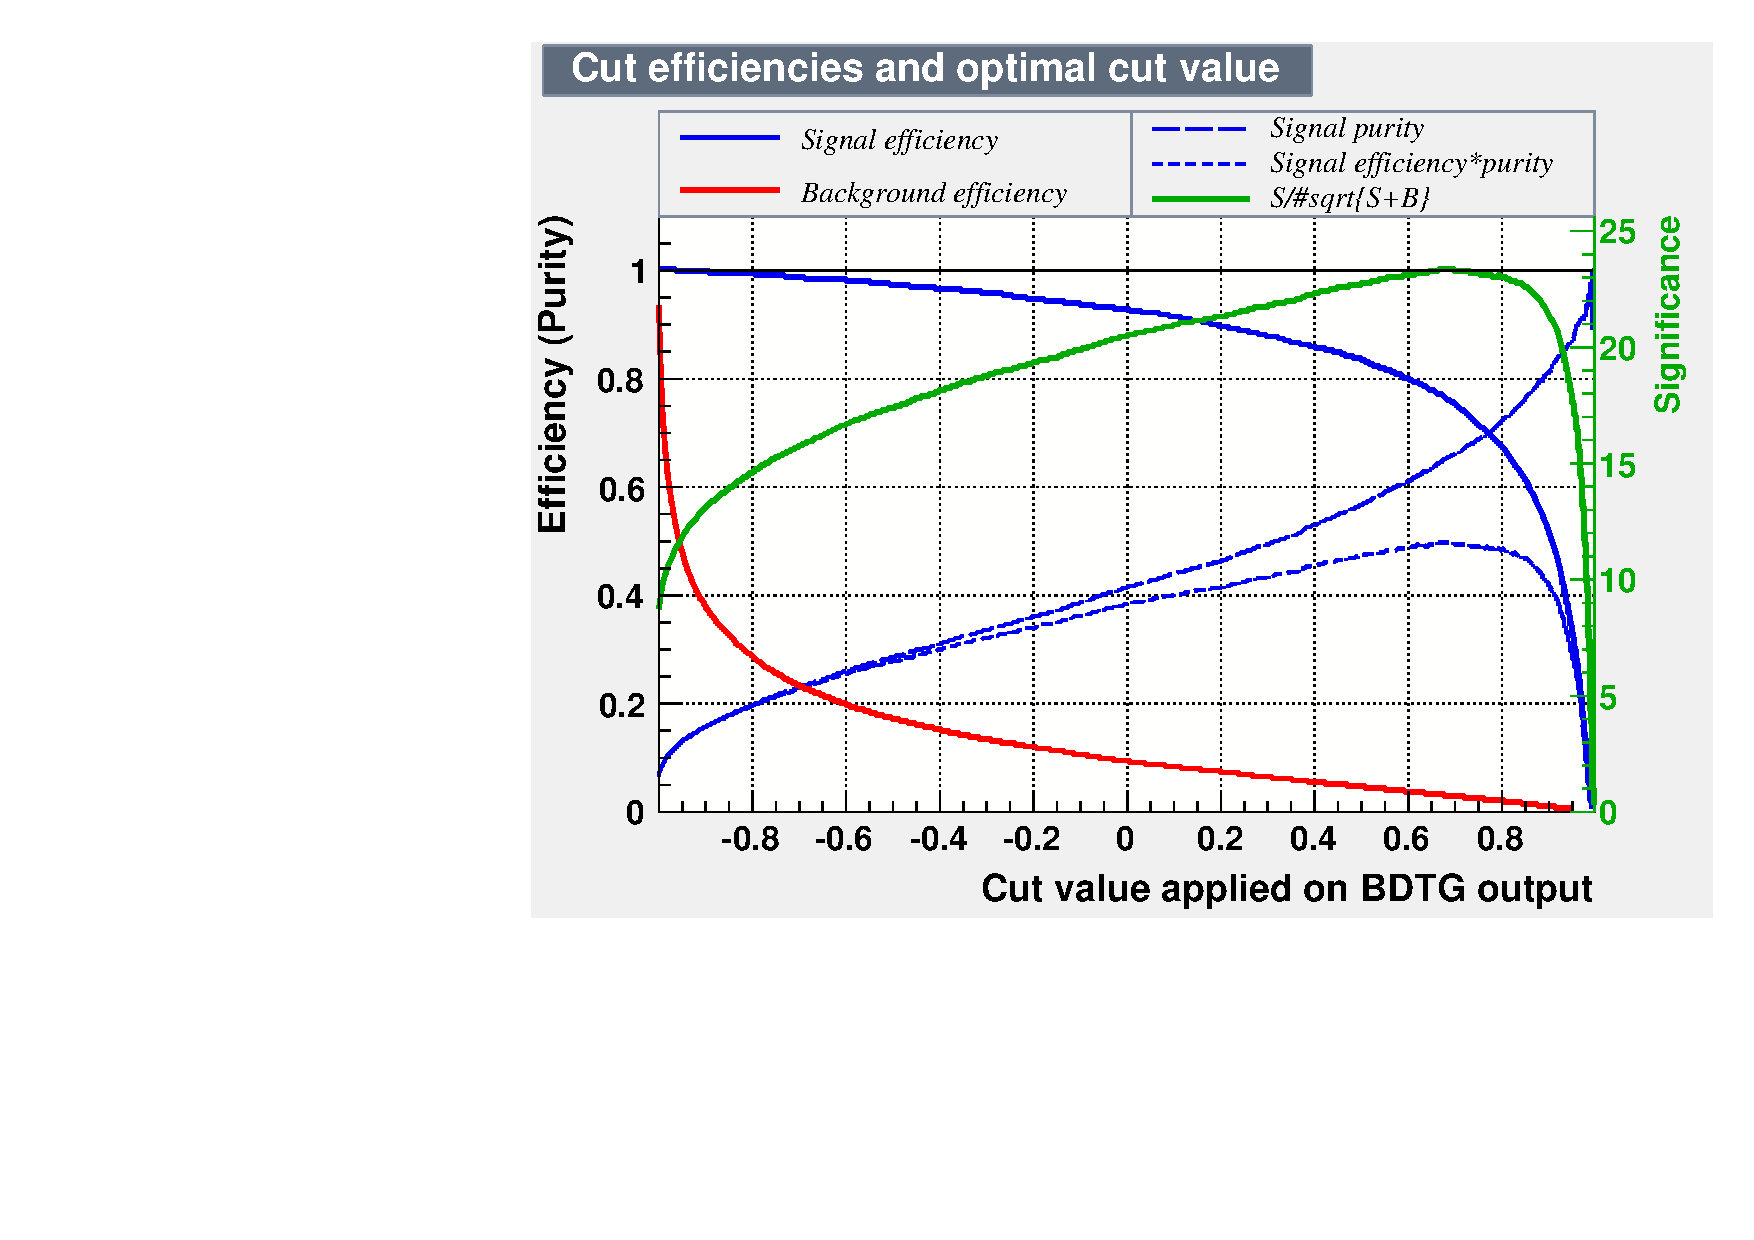
\includegraphics[height=7.4cm,width=0.7\textwidth]{figs/BDT_CutEfficiency.pdf}
%\vspace*{-0.2cm}
\caption{Efficiency and purity curves for (blue) signal, (red) background and the (green) FoM curve, as a function of the chosen cut value.}
\label{fig:BDT_Efficiency}
\end{figure}


\section{Models for signal and background components in invariant mass spectrum}
\label{sec: model}

The expected Signal shape, as well as the expected shape for the combinatorial and physical backgrounds have to be known in order to properly describe the invariant mass distribution of 
$\Bs\to\Ds\kaon\pion\pion$ and $\Bs\to\Ds\pion\pion\pion$ candidates.

\subsection{Signal model}
\label{subsec: signalmodel}
The mass distribution of $\Bs\to\Ds\kaon\pion\pion$ signal is modeled using two gaussian functions, which share the same mean $\mu$, but are allowed to have different widths $\sigma_{1}$ and $\sigma_{2}$. 
Another double gaussian is used to account for the contribution of $\B^{0}\to\Ds\kaon\pion\pion$ decays, which are also present in the $m(\Ds\kaon\pion\pion)$ spectrum. 
All parameters of both double gaussians except the core width $\sigma_{1}$ \comment{Why is it fixed and to what? } are allowed to float in the nominal fit. \newline
The same approach is used to describe the invariant mass distribution of $\Bs\to\Ds\pion\pion\pion$ candidates. 
A double gaussian is used to model this signal shape, all parameters except the core width $\sigma_{1}$ are allowed to float.

\subsection{Background models for $\m(\Ds\pion\pion\pion)$} 
\label{subsec: BkginNorm}
Different background sources arise in the invariant mass spectrum of candidates for the normalization mode. \newline
The following backgrounds have to be accounted for:
\begin{itemize}

\item combinatorial background: This contribution arises from either a real $\Ds$, which is paired with random tracks to form the $\Bs$ candidates, or via real $X_{d}$'s, which are combined with three tracks that fake a $\Ds$ candidate to form a fake $\Bs$.   

\item Partially reconstructed $\Bs\to\Ds^{*}\pion\pion\pion$ decays, with $\Ds^{*}\to\Ds\gamma$ or $\Ds^{*}\to\Ds\piz$, where the $\gamma$/$\piz$ is not reconstructed in the decay chain. 

\end{itemize}

In both cases of combinatorial background, the distribution in the invariant mass spectrum of $\Bs$ candidates is expected to be smooth and decrease with higher masses. 
Therefore, one exponential function is used to model these contributions. \newline
The shape of the  $\Bs\to\Ds^{*}\pion\pion\pion$ contribution is expected to be peaking in the $m(\Ds\pion\pion\pion)$ spectrum, with large tails due to the missing momentum, which is carried away by the $\piz$ or $\gamma$. 
We rely on simulation to estimate the shape of this contribution. 

\begin{figure}[h]
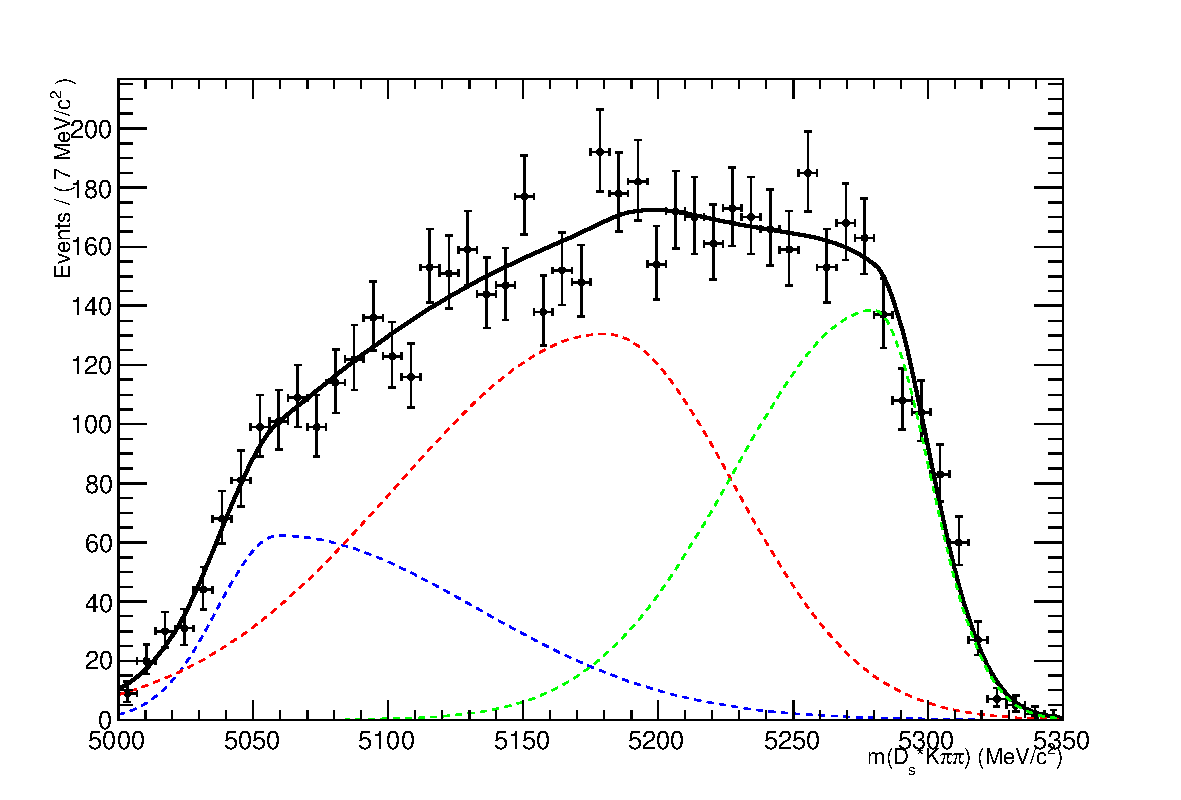
\includegraphics[height=8.cm,width=0.80\textwidth]{figs/Bs2Dsstartpipipi.pdf}
\caption{Invariant mass distribution of simulated $\Bs\to\Ds^{*}\pion\pion\pion$ events, where the $\gamma$/$\piz$ is excluded from the reconstruction. 
A fit of the sum of three bifurcated gaussians to this distribution is overlaid.}
\label{fig: BsDsstar3piMC}
\end{figure}

Figure \ref{fig: BsDsstar3piMC} shows the fit of the sum of three bifurcated gaussians to the invariant mass distribution of simulated $\Bs\to\Ds^{*}\pion\pion\pion$ event. 
The pion or photon from $\Ds^{*}\to\Ds(\gamma/\piz)$ is excluded from the reconstruction. The obtained shape parameters are used as input values for the nominal $m(\Ds\pion\pion\pion)$ mass fit. 
The yield of this contribution is directly determined in the nominal fit. 


\subsection{Background models for $m(\Ds\kaon\pion\pion)$}
For the signal channel, the following background sources have to be considered:

\begin{itemize}

\item combinatorial background: Same contributions as discussed in Sec. \ref{subsec: BkginNorm}.

\item Partially reconstructed $\Bs\to\Ds^{*}\kaon\pion\pion$ decays, with $\Ds^{*}\to\Ds\gamma$ or $\Ds^{*}\to\Ds\piz$, where the $\gamma$/$\piz$ is not reconstructed in the decay chain. 

\item Partially reconstructed $\Bz\to\Ds^{*}\kaon\pion\pion$ decays, with $\Ds^{*}\to\Ds\gamma$ or $\Ds^{*}\to\Ds\piz$, where the $\gamma$/$\piz$ is not reconstructed in the decay chain.

\item miss-identified $\Bs\to\Ds\pion\pion\pion$ decays, where one of the pions is wrongly identified as a kaon $\pion\rightarrow\kaon$.  

\item miss-identified, partially reconstructed $\Bs\to\Ds^{*}\pion\pion\pion$ decays, where one of the pions is wrongly identified as a kaon $\pion\rightarrow\kaon$ and the $\gamma$/$\piz$ from $\Ds^{*}\to\Ds\gamma$/$\piz$ is 
not reconstructed.

\end{itemize}

Again the combinatorial background is expected to be flat in the spectrum of the invariant mass of $\Bs\to\Ds\kaon\pion\pion$ candidates. An exponential function is used to model this contribution.\newline
The shape of the partially reconstructed $\Bs$/$\Bz\to\Ds^{*}\kaon\pion\pion$ background is taken from simulation. 
\comment{I think we take them from the normalization mode}
A MC sample of $\Bs\to\Ds^{*}\kaon\pion\pion$ events, where the $\gamma$/$\piz$ is excluded from the reconstruction, is generated. 
The sum of three bifurcated gaussians is then fitted to the mass distribution of $\Bs$ candidates. The distribution and the overlaid fit is shown in Fig. \ref{fig: BsDsstarKpipiMC}.  

\begin{figure}[h]
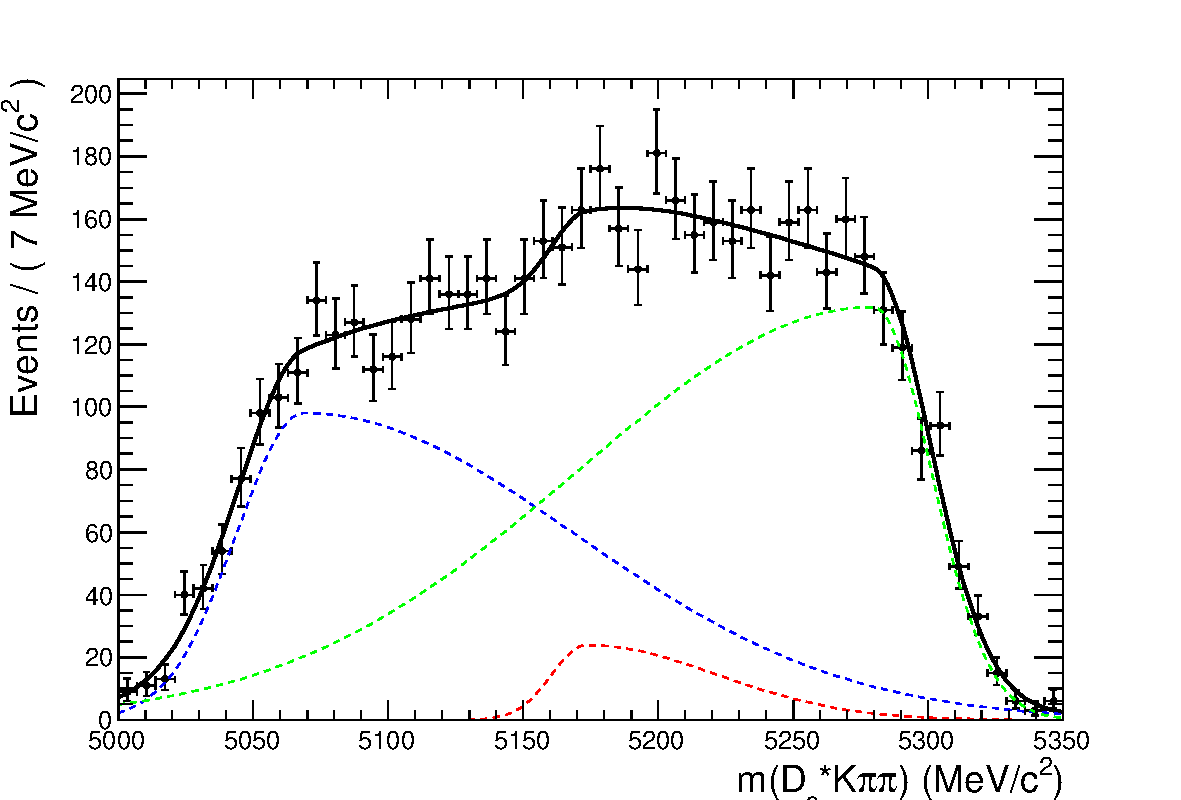
\includegraphics[height=8.cm,width=0.80\textwidth]{figs/Bs2DsstartKpipi.pdf}
\caption{Invariant mass distribution of simulated $\Bs\to\Ds^{*}\kaon\pion\pion$ events, where the $\gamma$/$\piz$ is excluded from the reconstruction. 
A fit of the sum of three bifurcated gaussians to this distribution is overlaid.}
\label{fig: BsDsstarKpipiMC}
\end{figure}

The obtained shape parameters are used as input values for the nominal $m(\Ds\kaon\pion\pion)$ mass fit. For the contribution of the $\Bz\to\Ds^{*}\kaon\pion\pion$ background, the same shape is used, but the means $\mu_{i}$ of the bifurcated gaussians are shifted down by $m_{\Bs} - m_{\Bz}$ \cite{Agashe:2014kda}. The yield of both contributions are directly determined in the nominal fit. \newline
To determine the shape of miss-identified $\Bs\to\Ds\pion\pion\pion$ candidates in the $m(\Ds\kaon\pion\pion)$ spectrum, we take a truth matched signal MC sample of our normalization channel. 
We then use the PIDCalib package to determine the $\pion\rightarrow\kaon$ fake rate. For every candidate in our MC sample, a $p$ and $\eta$-dependent event weight is computed and assigned. 
We flip the particle hypothesis from pion to kaon for the $\pion$ with the biggest miss-ID weight for each event and recompute the invariant $\Bs$ mass. This distribution is then modelled using two crystal ball functions. 
The distribution and fit is shown in Fig. \ref{fig: BsDspipipiMCmissID}(left). 

\begin{figure}[h]
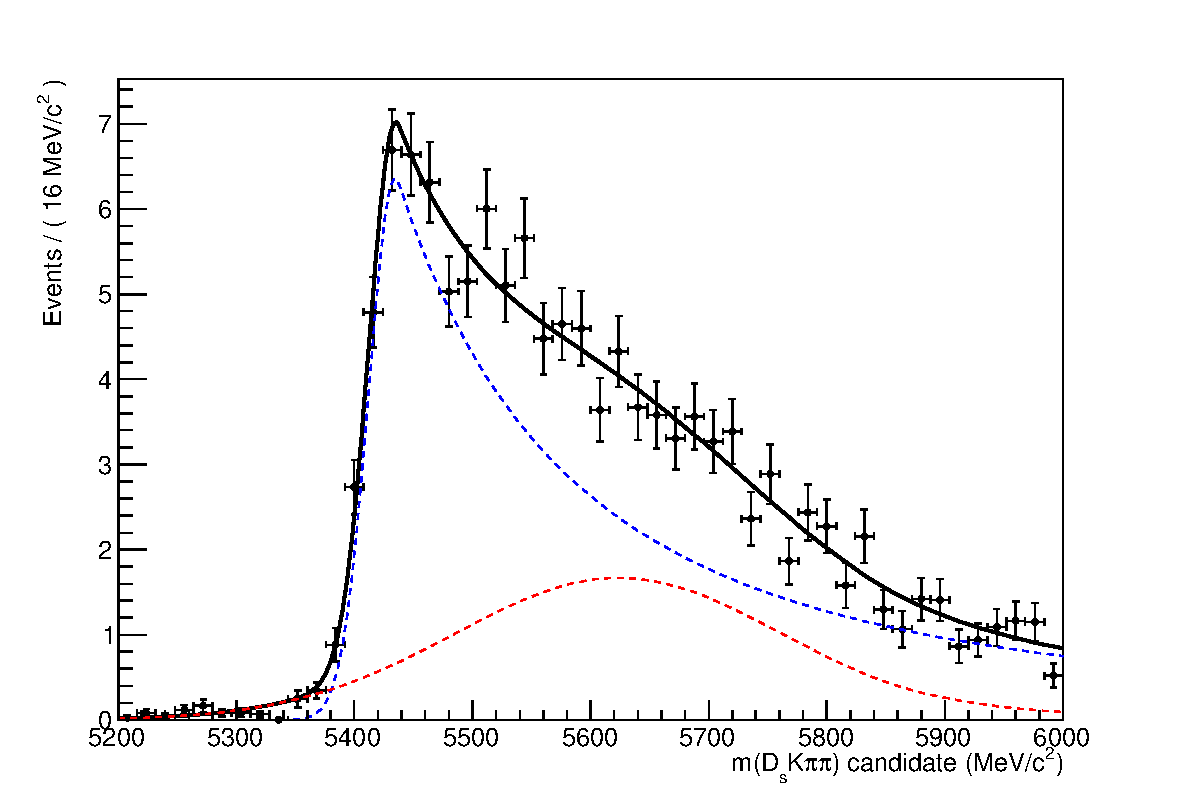
\includegraphics[height=6.cm,width=0.45\textwidth]{figs/Bs2Dspipipi_as_DsKpipi.pdf}
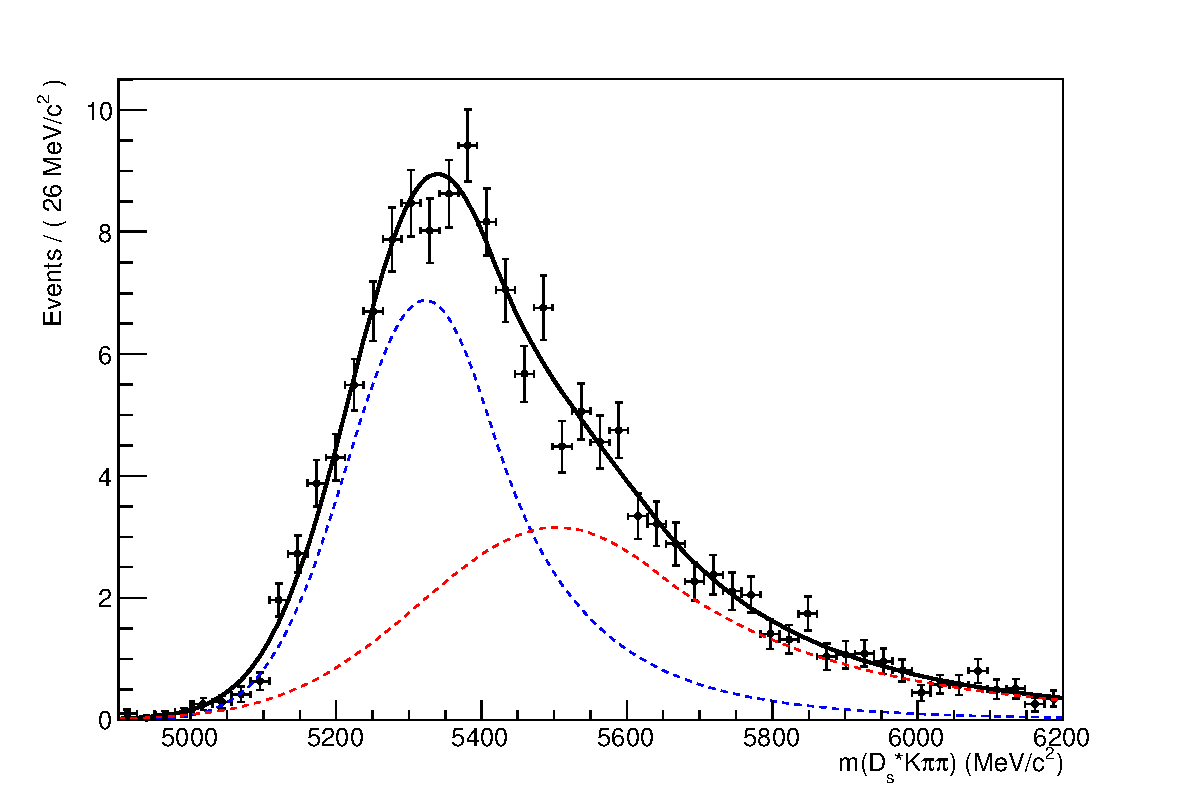
\includegraphics[height=6.cm,width=0.45\textwidth]{figs/Bs2Dsstarpipipi_as_DsKpipi.pdf}
\caption{Invariant mass distribution of (left) simulated $\Bs\to\Ds\pion\pion\pion$ events, where one of the $\pion$'s is reconstructed as a $\kaon$ and the miss-ID probability for each event is taken into account. 
The corresponding distribution for simulated $\Bs\to\Ds^{*}\pion\pion\pion$ events, where the $\gamma$/$\piz$ from the $\Ds^{*}$ is excluded from reconstruction, is shown on the right.
A fit of the sum of two crystal ball functions to each of these distributions is overlaid.}
\label{fig: BsDspipipiMCmissID}
\end{figure}
 
The expected yield of miss-identified $\Bs\to\Ds\pion\pion\pion$ candidates in the $m(\Ds\kaon\pion\pion)$ spectrum is computed by multiplying the fake probability of $\propto3.2\%$, which is derived from PIDCalib, by the yield of $\Bs\to\Ds\pion\pion\pion$ signal candidates, determined in the nominal mass fit of our normalization channel.  \newline
In the same way as mentioned above, we can determine the rate of miss-identified, partially reconstructed $\Bs\to\Ds^{*}\pion\pion\pion$ decays in our sample of $\Bs\to\Ds\kaon\pion\pion$ decays using PIDCalib and a MC sample of $\Bs\to\Ds^{*}\pion\pion\pion$ events. The invariant mass distribution we obtain when we exlude the $\gamma$/$\piz$, flip the the particle hypothesis $\pion\rightarrow\kaon$ and apply the event weights given by the fake rate, is shown in Fig. \ref{fig: BsDspipipiMCmissID} (right). The fit of two crystal ball functions to this distribution is overlaid. 
The yield of this contribution is determined from the yield of $\Bs\to\Ds^{*}\pion\pion\pion$ candidates in the nominal mass fit of our normalization channel, multiplied by the miss-ID probability of $\propto 3.6\%$.



\section{Massfits for signal and normalization channel}
\label{sec: fitting}

This section describes the nominal fits to the invariant mass distribution of $\Bs\to\Ds\kaon\pion\pion$ and $\Bs\to\Ds\pion\pion\pion$ candidates after all selection steps, described in the previous Sections, are applied. 
The obtained yields are summarized in Tab. \ref{tab: SigYields}.

\subsection{Fit to $\Bs\to\Ds\pion\pion\pion$ candidates}
\label{subsec: NormFit}

An unbinned maximum likelihood fit is performed to the invariant mass distribution of $\Bs\to\Ds\pion\pion\pion$ candidates. 
As discussed in Sec. \ref{subsec: signalmodel}, the fit is given as the sum of the double gaussian signal model, the sum of three bifurcated gaussians to model the partially reconstructed $\Bs\to\Ds^{*}\pion\pion\pion$ background, as well as an exponential to account for combinatorial background. The invariant mass distribution and the fit to it is shown in Fig. \ref{fig: BsDs3piFit}.

\begin{figure}[h]
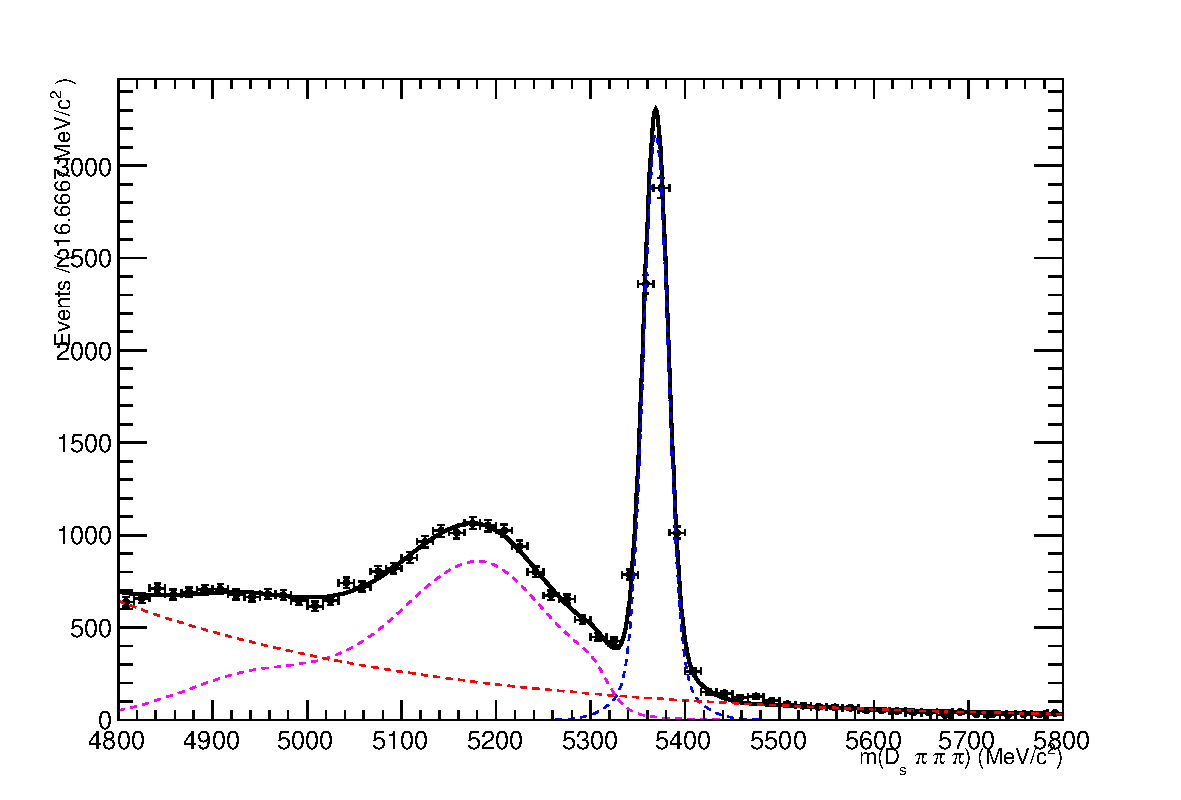
\includegraphics[height=7.cm,width=0.49\textwidth]{figs/3pi_BmassFit_11.pdf}
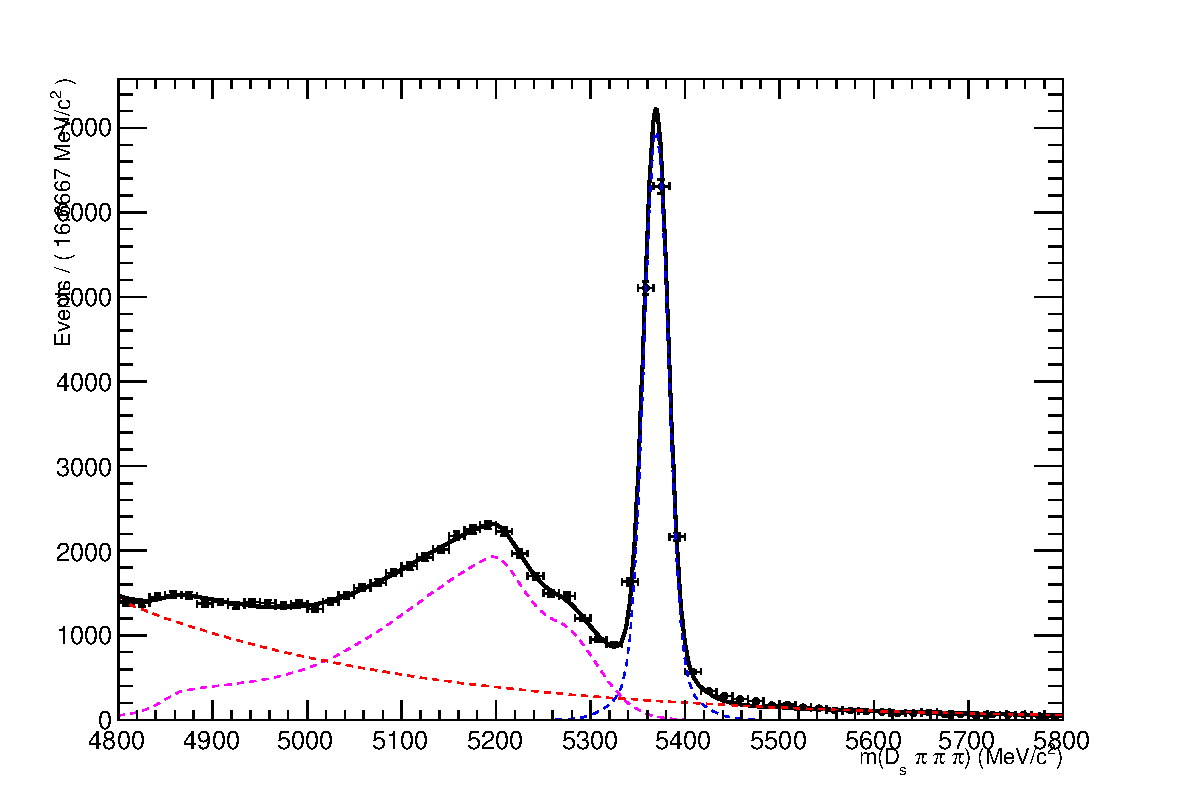
\includegraphics[height=7.cm,width=0.49\textwidth]{figs/3pi_BmassFit_12.pdf}
\caption{Invariant mass distribution of $\Bs\to\Ds\pion\pion\pion$ candidates for (left) 2011 and (right) 2012 data.
A fit described in the text is overlaid. The dashed lines show the (green) partially reconstructed and (red) combinatorial background, as well as the (blue) signal component.}
\label{fig: BsDs3piFit}
\end{figure}

The determined number of $\Bs\to\Ds\kaon\pion\pion$ decays is $7173 \pm 115$ for 2011 data and $15640 \pm 151$ for 2012 data. 
The determined yield for the partially reconstructed $\Bs\to\Ds^{*}\pion\pion\pion$ background is  (2011) $13685 \pm 449$ and (2012)  $28702e+04 \pm 573$, 
while the yield for the combinatorial background is (2011) $12193 \pm 457$ and (2012) $25212 \pm 564$.



\subsection{Fit to $\Bs\to\Ds\kaon\pion\pion$ candidates}
\label{subsec: SigFit}

\begin{figure}[h]
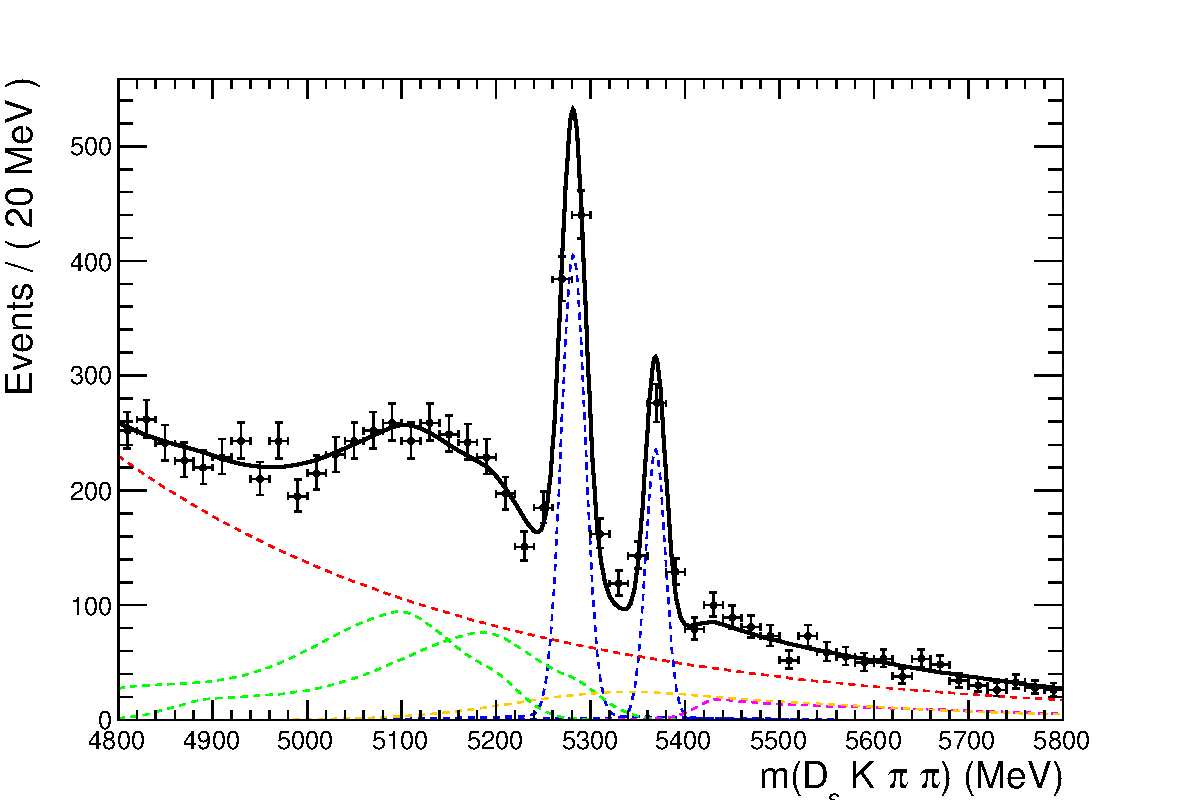
\includegraphics[height=7.cm,width=0.49\textwidth]{figs/BmassFit_11.pdf}
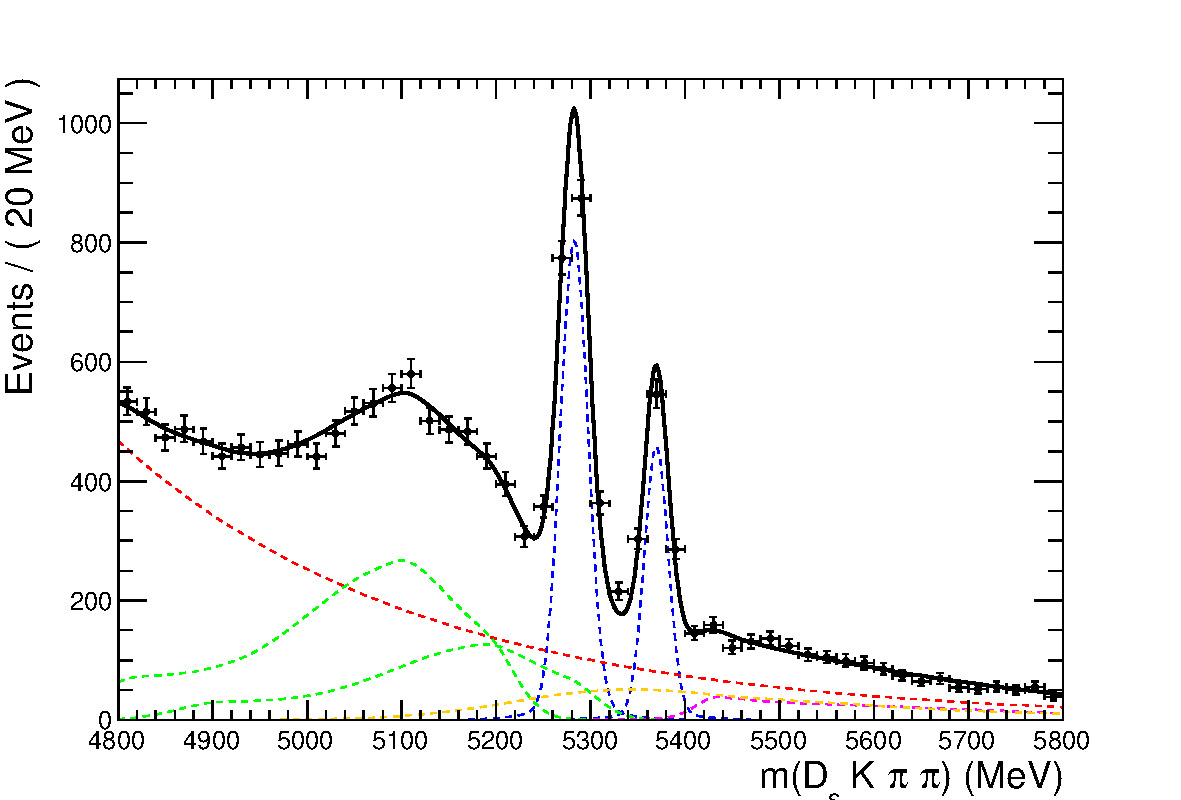
\includegraphics[height=7.cm,width=0.49\textwidth]{figs/BmassFit_12.pdf}
\caption{Invariant mass distribution of $\Bs\to\Ds\kaon\pion\pion$ candidates for (left) 2011 and (right) 2012 data.
A fit described in the text is overlaid. The dashed lines show the (green) partially reconstructed and (red) combinatorial background, as well as the (blue) signal component. 
Additional, the dashed magenta line depicts the miss-ID background and the dashed yellow line shows the miss-identified, partially reconstructed background component.}
\label{fig: BsDsKpipiFit}
\end{figure}


Fig. \ref{fig: BsDsKpipiFit} shows the invariant mass distribution of $\Bs\to\Ds\kaon\pion\pion$ candidates. 
A unbinned maximum likelihood fit is overlaid, which consists of two double gaussian models for the $\Bz$ and $\Bs$ signal, two sums of three bifurcated gaussians for the $\Bs$/$\Bz\to\Ds^{*}\kaon\pion\pion$ partially reconstructed background contributions and two sums of double crystal ball functions for the single miss-ID $\Bs\to\Ds\pion\pion\pion$ and the partially reconstructed, miss-identified $\Bs\to\Ds^{*}\pion\pion\pion$ decays. \newline
The extracted signal yields are (2011) $332 \pm  27$ and (2012) $787 \pm 39$.  


\begin{table}[h]
\centering
\begin{tabular}{l c c}
Decay & yield 2011 & yield 2012\\
\hline
$\Bs\to\Ds\kaon\pion\pion$ &  $332 \pm  27$   &  $787 \pm 39$\\
$\Bs\to\Ds\pion\pion\pion$ &  $7173 \pm 115$  &  $15640 \pm 151$\\
\hline
\end{tabular}
\caption{Summary of signal yields from the fits to 2011 and 2012 data.}
\label{tab: SigYields}
\end{table}



\section{Efficiency corrections}

Several relative efficiency corrections are needed to measure the branching fraction of $\Bs\to\Ds\kaon\pion\pion$ with respect to $\Bs\to\Ds\pion\pion\pion$. Precise knowledge of the efficiency related to the detector acceptance, PID requirements, used trigger lines and offline selections are crucial for both, the determination of $\gamma$ and the branching ratio measurement.

\subsection{Relative efficiency for BR measurement}
For the branching ratio measurement, the relative efficiency is given by

\begin{equation} 
\epsilon_{rel} = \epsilon^{acc}_{rel}\cdot\epsilon^{sel}_{rel}\cdot\epsilon^{pid}_{rel},
\label{eq: relEff}
\end{equation}

where $\epsilon = \frac{\epsilon_{Norm}}{\epsilon_{Sig}}$ is the ratio of the efficiency for the signal and normalization mode. To evaluate these efficiencies, we rely on simulation. The three efficiencies given in Eq. \ref{eq: relEff} are:

\begin{itemize}

\item $\epsilon^{acc}_{rel}$: This is the relative efficiency due to the geometrical acceptance of the LHCb detector. All tracks are required to have a polar angle between 10 and 400 mrad and a minimal momentum of $|p| >$ 1.6 $\gevc$ in order to be recorded for further analysis. Since the particle species of one track differs between the signal and normalizaton mode, the efficiencies caused by the geometrical acceptance are expected to be different for the two channels.

\item $\epsilon^{sel}_{rel}$: The relative selection efficiency due to trigger and offline requirements. 

\item $\epsilon^{pid}_{rel}$: The relative PID efficiency due to the identification likelihood requirements for tracks from both modes. This is evaluated using WHATEVER PIDCALIB MAGIC.

\end{itemize}

 Using the definition given in Eq. \ref{eq: relEff}, the branching ratio can be expressed as

\begin{equation}
\frac{\mathcal{B}(\Bs\to\Ds\kaon\pion\pion)}{\mathcal{B}(\Bs\to\Ds\pion\pion\pion)} = \frac{\mathcal{Y}(\Bs\to\Ds\kaon\pion\pion)}{\mathcal{Y}(\Bs\to\Ds\pion\pion\pion)},
\cdot \epsilon_{rel}
\label{eq: BRwEff}
\end{equation} 

where $\mathcal{Y}(x)$ represents the yield of the respective channel. \newline
Some further bla bla.

\begin{table}[h]
\centering
\begin{tabular}{l c c}
Efficiency ($\%$) & $\Bs\to\Ds\kaon\pion\pion$ & $\Bs\to\Ds\pion\pion\pion$\\
\hline
2011 $\epsilon^{acc}$ & xxx & yyy\\
2012 $\epsilon^{acc}$ & xxx & yyy\\
2011 $\epsilon^{sel}$ & 0.893 & yyy\\
2012 $\epsilon^{sel}$ & 0.794 & yyy\\
2011 $\epsilon^{pid}$ & 74.88 $\pm$ 0.85 & 92.64 $\pm$ 0.47\\
2012 $\epsilon^{pid}$ & 74.30 $\pm$ 0.85 & -\\
\hline
2011 total $\epsilon$ & z & zz\\
2012 total $\epsilon$ & z & zz\\
\hline
\end{tabular}
\caption{Efficiencies due to the detector accpetance, selection requirements and PID cuts for the signal and normalization mode. All values are obtained using simulated events.}
\label{tab: effTab}
\end{table}







\section{Systematic uncertainties}
\label{sec:Systematics}


This section covers all relevant systematic uncertainties on the measured observables.
In particular, the model dependent description of the invariant $\Bs$ mass spectrum, the parametrization of the time acceptance using cubic splines, 
as well as the scaling of the time resolution and tagging calibration are potential sources of systematic errors. 
The largest contribution of systematic uncertainty is expected to appear in the choice of amplitudes entering the model to describe the 5 dimensional phase space, discussed in Section \ref{sec:fullFit}.

\subsection{Models for $\Bs$ mass distribution}
\label{subsec:SystMass}

The statistical subtraction of the residual background \cite{Pivk:2004ty}, left after the full selection, relies on the correct description of the invariant $\Bs$ mass distribution.
Since the choice of signal and background models is not unique, alternative descriptions which lead to slightly different yields for the signal and background components are available. 
The difference in yields could result in shifted values for the measured observables and are therefore treated as systematic uncertainty. \newline

\subsubsection{Signal model}

The Johnson's SU function which is used as nominal signal model is replaced by a double Crystal Ball \cite{CB}. 
The crystal ball model is given by a gaussian core with an exponential tail on one side. 
Choosing a double Crystal Ball allows for asymmetric tails in a slightly different way compared to the Johnson's SU function. 
Table xXx summarizes the observed differences in signal and background yields.

\subsubsection{Background model}

For the description of the partially reconstructed background, 
a combination of the RooHILLdini and RooHORNsdini model [REF HERE] is used instead of the nominal model of three bifurcated gaussians. 
The HORNSdini model is used to describe the $\Bs\to\Ds^{*}[\to\Ds(\piz)] X_{s/d}$ decay, where the brackets around the $\piz$ indicate that it is missed in the reconstruction. 
The $\Ds^{*}\to\Ds\piz$ decay is a Vector $\to$ Scalar-Scalar ($1^{-}\to 0^{-}0^{-}$) transition. 
Using the helicity of the $\Ds$, one can show that this results in a double-peak structure in the reconstructed $\Bs$ mass. 
Therefore, the HORNSdini shape consists of a gaussian-like double-peak structure:

\begin{equation}
HORNS(m_{\Bs}) = \int^{b}_{a} dm_{\Bs}\left(m_{\Bs} - \frac{a+b}{2} \right)^{2}\mathcal{DG}(m_{\Bs}\vert\mu,\sigma,f_{G})\left(\frac{1-\zeta}{b-a}m_{\Bs} + \frac{b\zeta - a}{b - a} \right),
\label{eq:HORNS}
\end{equation}

where a and b are the kinematic endpoins of the distribution and $\zeta$ is the positive, real fraction of the two peak hights. Additionaly, the shape is convoluted with a gaussian to account for resolution effects.

The HILLdini model parametrizes the invariant mass shape of $\Bs\to\Ds^{*}[\to\Ds(\gamma)] X_{s/d}$ candidates, where the $\gamma$ is not reconstructed.
Contrary to the previously discussed process, the $Ds^{*}\to\Ds\gamma$ is a Vector $\to$ Scalar-Vector ($1^{-} \to 0^{-} 1^{-}$) transition. 
From helicity arguments, the expected shape in the mass distribution of $\Bs$ candidates follows a parabolic curve without any peaking structure.
To accommodate for this shape, the HILLdini model consists of a parabolic curve between the kinematic endpoints a \& b: 


\begin{equation}
HILL(m_{\Bs}) = \begin{cases} -(m_{\Bs} - a)(m_{\Bs} - b),& \mbox{for } a < m_{\Bs} < b \\
 0, &  otherwise. \end{cases}
\label{eq:HILLS}
 \end{equation}

This shape is convoluted with the same gaussian resolution function used for the HORNSdini model.
The resulting differences in yields is shown in Table xXx. \newline


To study systematic uncertainties originating from the description of the combinatorial background, the nominal second order polynomial is replaced by an exponential function. 
The changes in signal and background yields after refitting with this alternative shape are shown in Table xXx. \newline

\subsubsection{Systematic effect on observables}

The shift of the central values of the observables in the full fit when using sWeights obtained from a combination of alternative models, 
as well as using only one alternative model for the signal/comb.background/part.reco.background and keeping the nominal model for the other parts,
is shown in Table yYy. We conservatively choose the biggest variation as systematic uncertainty from the modelling of the invariant $\Bs$ mass spectrum.



\subsection{Decay-time acceptance}
\label{subsec:SystTime}

To investigate the systematic uncertainty related to the decay-time dependent efficiency, we vary our parametrization of the acceptance using cubic splines.
This is explicitly done by choosing slightly different knot positions, 
varying the spline coefficients at the nominal positions within their statistical uncertainties and adding/subtracting knots in the range $0.4\ps < t < 11\ps$.
Additionaly, an adaptive binning scheme is used to determine the knot positions in a way that roughly equal amounts of data is covered between two knots.
Strictly speaking, the variation of the spline coefficients within their uncertainty gives the statistical uncertainty of the decay-time acceptance parametrization.
For the presented measurement, this is done using the Cholesky decomposition  \cite{Golub:1996:MC:248979} of the covariance matrix of coefficients $c_{i}$, 
generating toy splines with randomized coefficient values $c_{i,toy}$ from this decomposition and refitting using the toy spline.  
Furthermore, the fit to the decay-time distribution of signal $\Bs\to\Ds\pion\pion\pion$ candidates, used to determine the spline parametrization, is reiterated with varying fixed/constrained values for $\DGs$.


\subsubsection{Varition of knot positions}
The nominal knot positions are changed to be:

\[ k_{alt1}(t) =  [0.5\mbox{ } 1 \mbox{ }1.5 \mbox{ }2 \mbox{ }3 \mbox{ }6 \mbox{ }9.5], 
\mbox{ } k_{alt2}(t) =  [0.5 \mbox{ } 1\mbox{ }  1.5 \mbox{ } 2 \mbox{ } 3\mbox{ }  9\mbox{ } 11],  
\mbox{ } k_{adaptive}(t) =  [0.7\mbox{ } 1.2\mbox{ } 1.7\mbox{ } 2.2\mbox{ } 6.3] \]


\subsubsection{Variation of spline coefficients}

Due to the sizeable correlation of the spline coefficients $c_{i}$ determined in Chapter \ref{sec:timeAcceptance}, 
the variations of the observables in the amplitude fit when changing one spline coefficient can not be added up in quadrature for all coefficients.
To simplify the problem, a Cholesky decomposition \cite{Golub:1996:MC:248979} is used to generate a set of uncorrelated vectors from the covariance matrix $A_{cov}$.
It can be shown that every Hermitian positive-definite matrix, such as $A_{cov}$, has a unique Cholesky decomposition of the form:

\begin{equation}
A_{cov} = L \cdot L^{T},
\label{eq:choleskyDecomp}
\end{equation}

where $L$ is a lower triangular matrix with real and positive diagonal entries and $L^{T}$ denotes the transpose of $L$. \newline

Given the four free spline coefficients which are determined from the fit described in \ref{sec:Acceptance}, $A_{cov}$ is a $4x4$ matrix. Therefore, the lower triangular matrix $L$ is of the form:

\begin{equation}
L = \begin{pmatrix}
v_{11} & 0 & 0 & 0 \\
v_{12} & v_{22} & 0 & 0 \\
v_{13} & v_{23} & v_{33} & 0\\ 
v_{14} & v_{24} & v_{34} & v_{44}
\end{pmatrix},
\label{eq:choleskyVectors}
\end{equation}


where $v_{ij}$ are real and positive numbers. $L$ contains four row vectors, which are by construction the four decorrelated modes of the covariant matrix $A_{cov}$. 
From this modes, one can form variations for each of the spline coefficients:

\begin{equation}
c_{i} = c_{nom,i} + \Sigma_{j} \left(r_{j} \cdot v_{ij} \right),
\label{eq:choleskyCoeffs}
\end{equation}

where $i=1..4$, $c_{i}$ is the i-th generated coefficient of the toy spline, $c_{nom,i}$ is the i-th coefficient determined from the nominal decay-time dependent fit to $\Bs\to\Ds\pion\pion\pion$, 
$r_{j}$ are normally distributed real random numbers from a distribution of unit width and $v_{ij}$ are the components of $L$ (where $i$ is the row index and $j$ the column index). \newline
We now generate four sets of 100 toy splines, where one of the four spline coefficients is varied each time using Eq. \ref{eq:choleskyCoeffs}. 
Thus, the time-dependent amplitude fit is repeated in total 400 times with a generated toy spline and the shift of the mean value of the physics observables over each of the $4\cdot100$ sets is quoted as 
uncertainty arising from $c_{i=1..4}$. The uncertainties are then added in quadrature to form the overall uncertainty due to the spline coefficients. Table \ref{table:Pulls_tDFit_noChol} summarizes the results of this study.

\begin{table}[hp!]
\centering
\caption{Pull parameters for CP coefficients from the toy studies for the time-dependent fit.}
\begin{tabular}{l | c | c}
\hline
Parameter & $\mu$ of pull distribution & $\sigma$ of pull distribution \\
\hline
\hline
C & 0.00271841 $\pm$ 0.00159745 & 0.0694972 $\pm$ 0.00127009 \\
D & -0.0115746 $\pm$ 0.00755454 & 0.331063 $\pm$ 0.00576761 \\
S & -0.00151265 $\pm$ 0.000852967 & 0.0378623 $\pm$ 0.000754181 \\
$\bar{D}$ & -0.0106657 $\pm$ 0.00746365 & 0.327998 $\pm$ 0.00581649 \\
$\bar{S}$ & -0.00152321 $\pm$ 0.000983966 & 0.0437459 $\pm$ 0.000849528 \\
\hline
\end{tabular}
\label{table:Pulls_tDFit_noChol}
\end{table}



\subsection{Decay-time resolution}

To study systematic effects originating from the scaling of the decay-time resolution $\sigma_{t}$, the decay-time distribution of fake $\Bs$ candidates using prompt $\Ds$ is described by single Gaussian function.
The resultions of the single Gaussians in the different bins of the per-event decay-time error can then be used to derive the scaling function in a straightforward way.
Since the distribution of the fake $\Bs$ decay time does not follow a perfect Gaussian distribution, two different approaches which either slightly overestimate or underestimate the decay time error are used:

\begin{itemize}

\item A double Gaussian is fit to the decay-time distributions of fake $\Bs$ candidates, but only the narrow with of the core Gaussian is considered to represent the time resolution in the respective bin. 
This method assumes that the other, broader Gaussian component does not represent the decay-time resolution of the signal $\Bs$ sample. Therefore the resolution is slightly underestimated in this case.

\item A singel Gaussian is fit to the decay-time distributions of fake $\Bs$ candidates in a wide range of $[-3\sigma_{t} : 1.5\sigma_{t}]$. 
Due to the tails of the distribution, which broaden the width of the Gaussian function, this method slightly overestimates the decay-time resolution.   

\end{itemize}

The widths of the single Gaussians from the fits performed with the two methods in bins of the per-event decay-time error is studied and a new resolution scaling function is derived for both cases: \newline

\begin{equation}
\sigma_{eff}^{core-Gauss}(\sigma_t) = \left(4.9  \pm 2.0 \right) \text{fs} + \left( 0.821 \pm 0.050 \right) \sigma_t
\label{eq:ResoSyst1}
\end{equation}

\begin{equation}
\sigma_{eff}^{single-Gauss}(\sigma_t) = \left(8.3  \pm 1.5 \right) \text{fs} + \left( 0.997 \pm 0.037 \right) \sigma_t
\label{eq:ResoSyst2}
\end{equation}

The scaling functions are shown in Fig. \ref{fig:SystscaleFactor} and the systematic uncertainty to the CP-observables is summarized in Table yYy.


    
\begin{figure}[h]
\centering
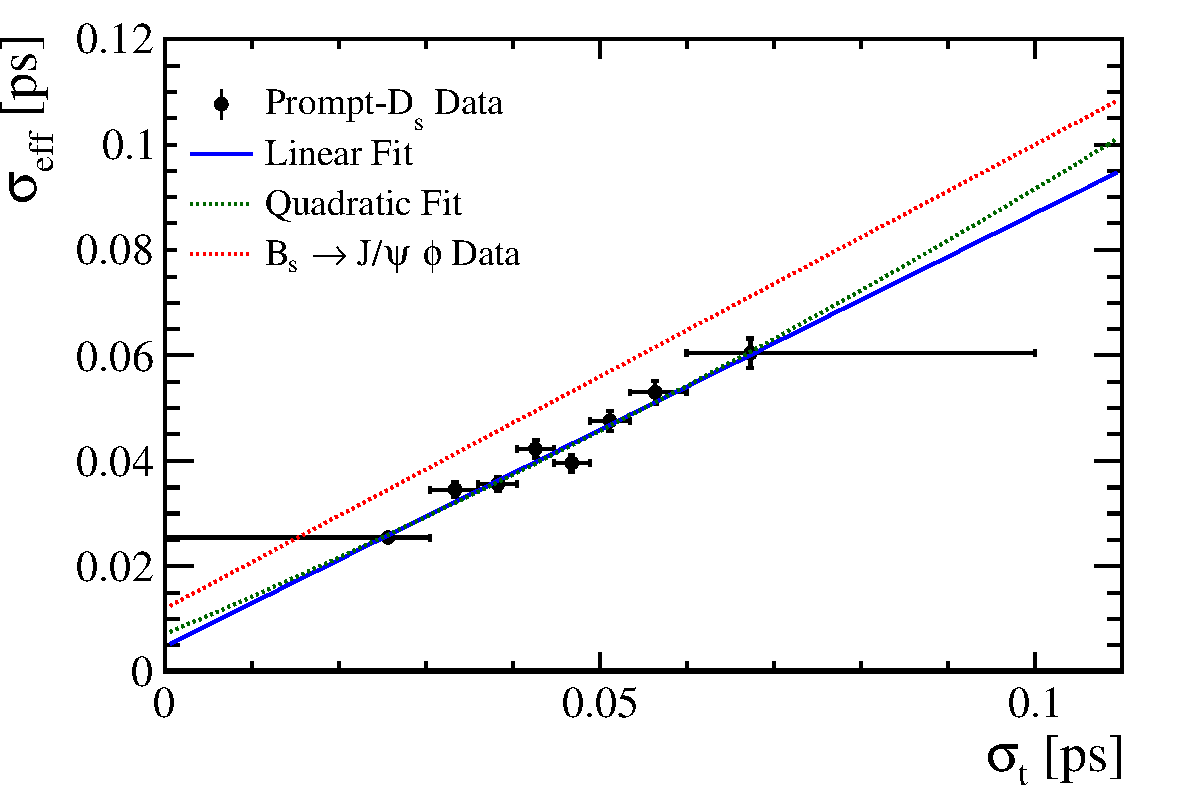
\includegraphics[height=!,width=0.49\textwidth]{figs/Resolution/ScaleFactor_Data_coreGauss.pdf}
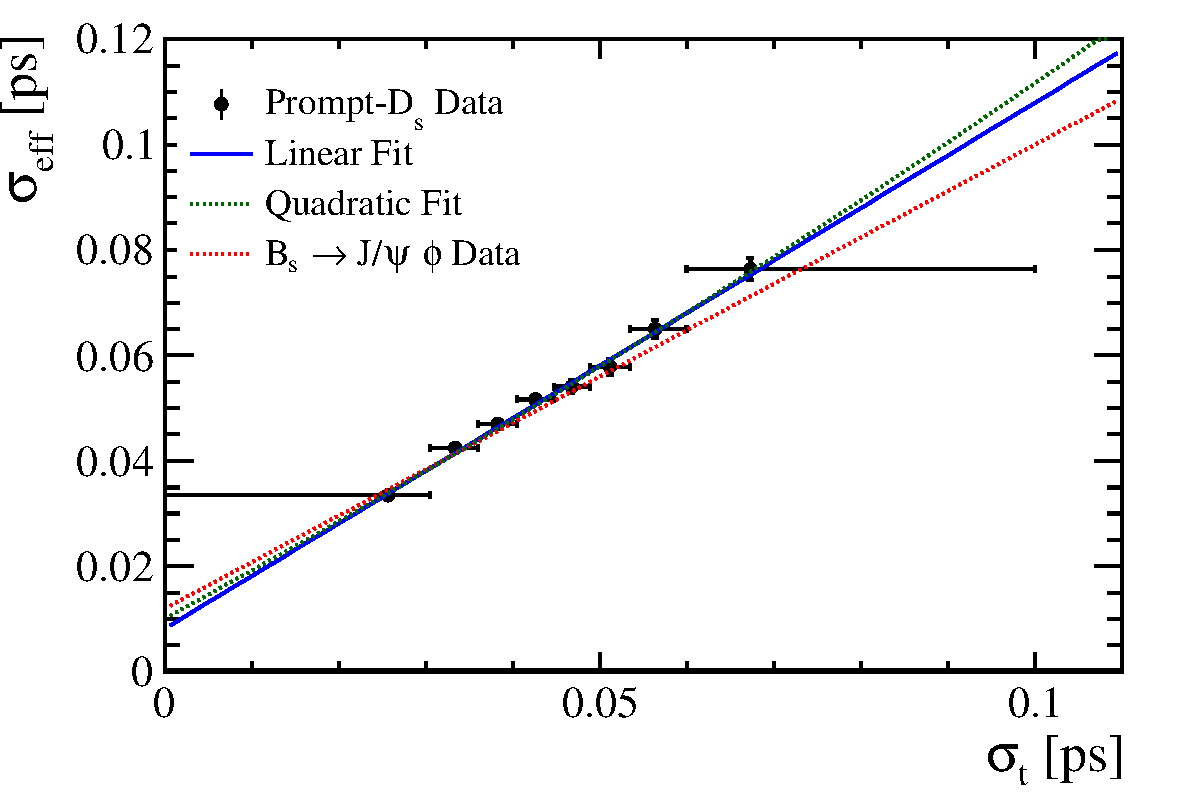
\includegraphics[height=!,width=0.49\textwidth]{figs/Resolution/ScaleFactor_Data_singleGauss.pdf}
\caption{The measured resolution $\sigma_{eff}$ as function of the per-event decay time error estimate $\sigma_t$ for fake $B_s$ candidates (Run-II data) 
when (left) only using the narrow gaussian width of the double gaussian fit model or (right) when determining the resolution using a single gaussian model.
The fitted calibration curve is shown in blue for both cases.}
\label{fig:SystscaleFactor}
\end{figure}


\subsection{Tagging calibration}



\subsection{Summary of systematic uncertainties}


\section{Results and summary}
\label{sec: results}

Using the definition of the branching ratio given in Eq. \ref{eq: BRwEff}, we compute from the measured yields and efficiencies:

\begin{equation}
\frac{\mathcal{B}(\Bs\to\Ds\kaon\pion\pion)}{\mathcal{B}(\Bs\to\Ds\pion\pion\pion)} = 0.056 \pm 0.003 \pm 0.003,
\label{eq: resultBR}
\end{equation}

where the uncertainties are statistical and systematical, respectively. \newline
The results are in good agreement with the first observation and BR measurement of the $\Bs\to\Ds\kaon\pion\pion$ decay, done with 1 $\invfb$ of 2011 LHCb data \cite{Blusk:2012it}.  
The number of signal events already exceeds one thousand candidates, although only the $\Ds\to\kaon\kaon\pion$ final state has been used for this analysis. 
Adding the $\Ds\to\pion\pion\pion$ final state, which is expected to contribute roughly 20 $\%$ of signal on top, makes this channel a promising prospect for a time-dependent $\gamma$ determination.



\newpage

\appendix

\section{Appendix}
\label{sec: appendix}

\subsection{Re-weghted MC observables}
\label{sec: mcvdata}
The following figures show the distributions of observables used during the multivariate selection stage, for data, monte carlo and re-weighted monte carlo.


%\begin{figure}[h]
%\includegraphics[height=6.cm,width=0.45\textwidth]{figs/.pdf}
%\includegraphics[height=6.cm,width=0.45\textwidth]{figs/.pdf}\\
%\includegraphics[height=6.cm,width=0.45\textwidth]{figs/.pdf}
%\includegraphics[height=6.cm,width=0.45\textwidth]{figs/.pdf}
%\caption{Comparison of data and simulated observables, before and after re-weighting 1.}
%\end{figure}


\subsection{Toys for normalization fit}
\label{sec: toysNorm}

To validate the fit model used to describe the $m(\Ds\pion\pion\pion)$ spectrum, we produce 1000 pseudo samples from our fit pdf and fit them with the same nominal pdf model. \newline
A pull of a certain fit parameter is defined as

\begin{equation}
p = \frac{x - x_{0}}{\Delta x},
\label{eq: pull}
\end{equation}  

where $x$ is the fitted value, $x_{0}$ the generated value and $\Delta x$ the uncertainty on $x$. 
Given the fit is correctly implemented and unbiased, one expects the distribution of the pulls for every fit parameter to be centered around 0, with a gaussian width of 1.


%\begin{figure}[h]
%\includegraphics[height=6.cm,width=0.45\textwidth]{figs/.pdf}
%\includegraphics[height=6.cm,width=0.45\textwidth]{figs/.pdf}\\
%\includegraphics[height=6.cm,width=0.45\textwidth]{figs/.pdf}
%\includegraphics[height=6.cm,width=0.45\textwidth]{figs/.pdf}
%\caption{Pull distributions for 1000 pseudo experiments, using the fit model for the normalization fit. Part 1.}
%\end{figure}


\newpage

\addcontentsline{toc}{section}{References}
\setboolean{inbibliography}{true}
\bibliographystyle{LHCb}
\bibliography{main,LHCb-PAPER,LHCb-CONF,LHCb-DP,LHCb-TDR}


%\newpage

% Author List ----------------------------                                                                                                                                                                                                                                                                                                
%  You need to get a new author list!                                                                                                                                                                                                                                                                                                    

%\input{LHCb_HD_authorlist_2014-06-20}
 
%\newpage
%% $Id: LHCb_authorlist.tex 78711 2015-08-06 07:54:32Z apuignav $
% ===============================================================================
% Purpose: example of authorlist for LHCb template
% Author:
% Created on: 2009-09-24
% ===============================================================================

%\documentclass[a4paper]{article}
%\setlength{\oddsidemargin}{0cm}
%\setlength{\evensidemargin}{0cm}
%\setlength{\textwidth}{16.5cm}
%\setlength{\parindent}{0cm}
%\begin{document}
\centerline{\large\normalfont\bfseries LHCb collaboration}
\begin{flushleft}
\small
%-- LHCb Authorlist, Example typesetting
%-- 
A.~N.~Other$^{1}$.\bigskip\newline{\it
\footnotesize
$ ^{1}$University of nowhere\\
}
%-- 
%-- 
\end{flushleft}
%\end{document}


%The author list for journal publications is generated from the Membership Database shortly after 'approval to go to paper' has been given.
%It will be sent to you by email shortly after a paper number has been assigned.
%The author list should be included already at first circulation,
%to allow new members of the collaboration to verify that they have been included correctly.
%Occasionally a misspelled name is corrected, or associated institutions become full members.
%Therefore an updated author list will be sent to you after the final EB review of the paper.
%In case line numbering doesn't work well after including the authorlist, try moving the \verb!\bigskip! after the last author to a separate line.


%The authorship for Conference Reports should be ``The LHCb                                                                                                                                                                                                                                                                                
%  collaboration'', with a footnote giving the name(s) of the contact
%  author(s), but without the full list of collaboration names.



\end{document}
